\documentclass[twocolumn,linenumbers]{aastex62}
%\documentclass{aastex62}
\usepackage{xspace}

%% The default is a single spaced, 10 point font, single spaced article.
%% There are 5 other style options available via an optional argument. They
%% can be envoked like this:
%%
%% \documentclass[argument]{aastex62}
%% 
%% where the layout options are:
%%
%%  twocolumn   : two text columns, 10 point font, single spaced article.
%%                This is the most compact and represent the final published
%%                derived PDF copy of the accepted manuscript from the publisher
%%  manuscript  : one text column, 12 point font, double spaced article.
%%  preprint    : one text column, 12 point font, single spaced article.  
%%  preprint2   : two text columns, 12 point font, single spaced article.
%%  modern      : a stylish, single text column, 12 point font, article with
%% 		  wider left and right margins. This uses the Daniel
%% 		  Foreman-Mackey and David Hogg design.
%%  RNAAS       : Preferred style for Research Notes which are by design 
%%                lacking an abstract and brief. DO NOT use \begin{abstract}
%%                and \end{abstract} with this style.
%%
%% Note that you can submit to the AAS Journals in any of these 6 styles.
%%
%% There are other optional arguments one can envoke to allow other stylistic
%% actions. The available options are:
%%
%%  astrosymb    : Loads Astrosymb font and define \astrocommands. 
%%  tighten      : Makes baselineskip slightly smaller, only works with 
%%                 the twocolumn substyle.
%%  times        : uses times font instead of the default
%%  linenumbers  : turn on lineno package.
%%  trackchanges : required to see the revision mark up and print its output
%%  longauthor   : Do not use the more compressed footnote style (default) for 
%%                 the author/collaboration/affiliations. Instead print all
%%                 affiliation information after each name. Creates a much
%%                 long author list but may be desirable for short author papers
%%
%% these can be used in any combination, e.g.
%%
%% \documentclass[twocolumn,linenumbers,trackchanges]{aastex62}
%%
%% AASTeX v6.* now includes \hyperref support. While we have built in specific
%% defaults into the classfile you can manually override them with the
%% \hypersetup command. For example,
%%
%%\hypersetup{linkcolor=red,citecolor=green,filecolor=cyan,urlcolor=magenta}
%%
%% will change the color of the internal links to red, the links to the
%% bibliography to green, the file links to cyan, and the external links to
%% magenta. Additional information on \hyperref options can be found here:
%% https://www.tug.org/applications/hyperref/manual.html#x1-40003
%%
%% If you want to create your own macros, you can do so
%% using \newcommand. Your macros should appear before
%% the \begin{document} command.
%%
\newcommand{\vdag}{(v)^\dagger}
\newcommand\aastex{AAS\TeX}
\newcommand\latex{La\TeX}

\newcommand{\Gray}{$\gamma$~ray\xspace}
\newcommand{\Grays}{$\gamma$~rays\xspace}
\newcommand{\GRays}{$\gamma$~Rays\xspace}
\newcommand{\gray}{$\gamma$-ray\xspace}
\newcommand{\unit}[1]{\,\mathrm{#1}\xspace}
\newcommand{\Fermi}{\emph{Fermi}\xspace}
\newcommand{\FermiLAT}{\emph{Fermi}~LAT\xspace}
\newcommand{\fermiLAT}{\emph{Fermi}-LAT\xspace}
\newcommand{\todo}[1]{\textbf{\textcolor{red}{#1}}}

%% Reintroduced the \received and \accepted commands from AASTeX v5.2
\received{\today}
\revised{January 7, 2019}
\accepted{Soon}
%% Command to document which AAS Journal the manuscript was submitted to.
%% Adds "Submitted to " the arguement.
\submitjournal{ApJ}

%% Mark up commands to limit the number of authors on the front page.
%% Note that in AASTeX v6.2 a \collaboration call (see below) counts as
%% an author in this case.
%
%\AuthorCollaborationLimit=3
%
%% Will only show Schwarz, Muench and "the AAS Journals Data Scientist 
%% collaboration" on the front page of this example manuscript.
%%
%% Note that all of the author will be shown in the published article.
%% This feature is meant to be used prior to acceptance to make the
%% front end of a long author article more manageable. Please do not use
%% this functionality for manuscripts with less than 20 authors. Conversely,
%% please do use this when the number of authors exceeds 40.
%%
%% Use \allauthors at the manuscript end to show the full author list.
%% This command should only be used with \AuthorCollaborationLimit is used.

%% The following command can be used to set the latex table counters.  It
%% is needed in this document because it uses a mix of latex tabular and
%% AASTeX deluxetables.  In general it should not be needed.
%\setcounter{table}{1}

%%%%%%%%%%%%%%%%%%%%%%%%%%%%%%%%%%%%%%%%%%%%%%%%%%%%%%%%%%%%%%%%%%%%%%%%%%%%%%%%
%%
%% The following section outlines numerous optional output that
%% can be displayed in the front matter or as running meta-data.
%%
%% If you wish, you may supply running head information, although
%% this information may be modified by the editorial offices.
\shorttitle{Gamma-ray variability of bright FSRQs}
\shortauthors{Meyer et al.}
%%
%% You can add a light gray and diagonal water-mark to the first page 
%% with this command:
% \watermark{text}
%% where "text", e.g. DRAFT, is the text to appear.  If the text is 
%% long you can control the water-mark size with:
%  \setwatermarkfontsize{dimension}
%% where dimension is any recognized LaTeX dimension, e.g. pt, in, etc.
%%
%%%%%%%%%%%%%%%%%%%%%%%%%%%%%%%%%%%%%%%%%%%%%%%%%%%%%%%%%%%%%%%%%%%%%%%%%%%%%%%%

%% This is the end of the preamble.  Indicate the beginning of the
%% manuscript itself with \begin{document}.

\begin{document}

\title{Characterizing the gamma-ray variability of the brightest flat spectrum radio quasars observed with the \emph{Fermi} LAT}

%% LaTeX will automatically break titles if they run longer than
%% one line. However, you may use \\ to force a line break if
%% you desire. In v6.2 you can include a footnote in the title.

%% A significant change from earlier AASTEX versions is in the structure for 
%% calling author and affilations. The change was necessary to implement 
%% autoindexing of affilations which prior was a manual process that could 
%% easily be tedious in large author manuscripts.
%%
%% The \author command is the same as before except it now takes an optional
%% arguement which is the 16 digit ORCID. The syntax is:
%% \author[xxxx-xxxx-xxxx-xxxx]{Author Name}
%%
%% This will hyperlink the author name to the author's ORCID page. Note that
%% during compilation, LaTeX will do some limited checking of the format of
%% the ID to make sure it is valid.
%%
%% Use \affiliation for affiliation information. The old \affil is now aliased
%% to \affiliation. AASTeX v6.2 will automatically index these in the header.
%% When a duplicate is found its index will be the same as its previous entry.
%%
%% Note that \altaffilmark and \altaffiltext have been removed and thus 
%% can not be used to document secondary affiliations. If they are used latex
%% will issue a specific error message and quit. Please use multiple 
%% \affiliation calls for to document more than one affiliation.
%%
%% The new \altaffiliation can be used to indicate some secondary information
%% such as fellowships. This command produces a non-numeric footnote that is
%% set away from the numeric \affiliation footnotes.  NOTE that if an
%% \altaffiliation command is used it must come BEFORE the \affiliation call,
%% right after the \author command, in order to place the footnotes in
%% the proper location.
%%
%% Use \email to set provide email addresses. Each \email will appear on its
%% own line so you can put multiple email address in one \email call. A new
%% \correspondingauthor command is available in V6.2 to identify the
%% corresponding author of the manuscript. It is the author's responsibility
%% to make sure this name is also in the author list.
%%
%% While authors can be grouped inside the same \author and \affiliation
%% commands it is better to have a single author for each. This allows for
%% one to exploit all the new benefits and should make book-keeping easier.
%%
%% If done correctly the peer review system will be able to
%% automatically put the author and affiliation information from the manuscript
%% and save the corresponding author the trouble of entering it by hand.

\correspondingauthor{Manuel Meyer}
\email{mameyer@stanford.edu}

\author[0000-0002-0738-7581]{Manuel Meyer}
\affil{Kavli}

\author{Jeffrey Scargle}
\affil{NASA Ames}

\author{Roger Blandford}
\affil{Kavli}

\author{The \emph{Fermi}-LAT Collaboration}
\affiliation{Flying from a low Earth orbit}

%% Note that the \and command from previous versions of AASTeX is now
%% depreciated in this version as it is no longer necessary. AASTeX 
%% automatically takes care of all commas and "and"s between authors names.

%% AASTeX 6.2 has the new \collaboration and \nocollaboration commands to
%% provide the collaboration status of a group of authors. These commands 
%% can be used either before or after the list of corresponding authors. The
%% argument for \collaboration is the collaboration identifier. Authors are
%% encouraged to surround collaboration identifiers with ()s. The 
%% \nocollaboration command takes no argument and exists to indicate that
%% the nearby authors are not part of surrounding collaborations.

%% Mark off the abstract in the ``abstract'' environment. 
\begin{abstract}

Almost 10 years of $\gamma$-ray observations with the \emph{Fermi} Large Area Terlescope (LAT) have revealed extreme  $\gamma$-ray outbursts from flat spectrum radio quasars (FSRQs), temporarily making these objects the brightest $\gamma$-ray emitters in sky. 
Yet, the location and mechanisms of the $\gamma$-ray emission remain elusive. 
To gain further insight into these questions, we characterize long-term variability and brightest flares of six FSRQs observed with the LAT.
Consecutively zooming in on the brightest flares, which we identify in an unbiased way through Bayesian Blocks and a hill-climbing algorithm, 
we find evidence for variability on timescales as short as minutes in four sources (3C279, PKS1510-089, CTA102, 3C454.3), which suggests extremely compact emission regions in the jet.
We do not find any signs for $\gamma$-ray absorption in the broad line region, which indicates that the $\gamma$-rays are produced away from the black hole by hundreds of gravitational radii. 
This is further supported by a cross-correlation analysis between $\gamma$-ray and radio light curves, which is compatible with a co-spatial production of $\gamma$~rays and radio emission at mm wavelengths in 3C454.3 and CTA102, located at distances $\gtrsim 1\,$pc from the central black hole. 
These distances are still consistent with the observed decay times of the brightest flares if the decay is caused by radiative cooling in external radiation fields.
However, the minute-scale variability is challenging to explain in such scenarios.
%The gamma-ray light curves of these sources on different temporal scales provide us with a rich data set that can be compared to theoretical models of emission and particle cooling scenarios.

\end{abstract}

%% Keywords should appear after the \end{abstract} command. 
%% See the online documentation for the full list of available subject
%% keywords and the rules for their use.
\keywords{editorials, notices --- 
miscellaneous --- catalogs --- surveys}

%% From the front matter, we move on to the body of the paper.
%% Sections are demarcated by \section and \subsection, respectively.
%% Observe the use of the LaTeX \label
%% command after the \subsection to give a symbolic KEY to the
%% subsection for cross-referencing in a \ref command.
%% You can use LaTeX's \ref and \label commands to keep track of
%% cross-references to sections, equations, tables, and figures.
%% That way, if you change the order of any elements, LaTeX will
%% automatically renumber them.
%%
%% We recommend that authors also use the natbib \citep
%% and \citet commands to identify citations.  The citations are
%% tied to the reference list via symbolic KEYs. The KEY corresponds
%% to the KEY in the \bibitem in the reference list below. 

\section{Introduction} \label{sec:intro}

More than half of the sources observed with the \Fermi Large Area Telescope (LAT) above 100\,MeV are active galaxies that produce particle outflows (jets) at almost the speed of light, which are closely aligned to the line of sight.\footnote{See e.g. \url{http://www.asdc.asi.it/fermi3fgl/}}
%Yet, the exact mechanism and location of \gray production inside such jets of these so-called blazars remain a controversially discussed topic in the literature~\cite{Madejski:2016oqg}.
The broadband electromagnetic radiation observed from these so-called blazars spans decades in energy from radio frequencies up to very-high energy \gray energies. 
It is often described with purely leptonic or a mixture of leptonic and hadronic emission models, involving both intrinsic and external radiation fields~\cite[e.g.,][and references therein]{Madejski:2016oqg}.
%It is often explained with either purely leptonic or mixture of hadronic and leptonic emission models. 
%In leptonic models, the low energy part of the spectral energy distribution (SED) is caused by synchrotron emission of relativistic electrons in magnetic fields, whereas the high energy end of the SED is attributed to inverse Compton scattering of electrons with either the synchrotron emission or external radiation fields. 
%In leptonhadronic models, the high energy emission can be due to proton-synchrotron radiation, or the creation of particle cascades produced in interactions of cosmic rays with ambient gas and radiation fields. 
%In leptonic models, the emission is due to synchrotron emission and inverse Compton scattering of the electrons with synchrotron emission or external radiation fields. In leptohadronic models the high energy emission can be either due to proton-synchrotron radiation or emission produced in particle cascades, which are initiated by cosmic-ray interactions with gas and radiation fields.
A common assumption is that the radiation is emitted by freshly accelerated   particles localized in ``plasmoids''  that move down the jet at relativistic speeds,
 leading to a strong doppler boost of the observed emission. 
Yet, the origin and location of such plasmoids remain unknown. 

Blazars also display variable emission at all observationally accessible time scales, limited only by signal-to-noise.
Surprisingly, at \gray energies, flux doubling times as low as minutes have been observed both in BL Lac-type objects and flat spectrum radio quasars (FSRQs) with ground-based Cherenkov telescopes and the \FermiLAT~\cite[e.g.][]{pks2155hess2007,pks1222magic2011,TheFermi-LAT:2016dss,2018ApJ...854L..26S}.
In these cases, causality arguments suggest extremely compact emission regions realized in, e.g., magnetic reconnection events or recollimation shocks~\cite[e.g.][]{Petropoulou:2016xat,Bodo:2017qqn}.
In particular for FSRQs, the observation of \Grays beyond 10\,GeV suggests that these compact dissipation sites are located at distances of hundreds of Schwarzschild  radii from the central super massive black hole. 
Otherwise, the \gray emission would be strongly attenuated in the interaction with UV and optical photons that are emitted from fast rotating clouds of ionized gas of the broad line region (BLR). 
Meeting these constraints is challenging for standard emission scenarios as extreme relativistic bulk motions of the plasma have to be invoked~\cite[e.g.,][]{TheFermi-LAT:2016dss}. 

After almost one decade of continuous all-sky observations, the \FermiLAT has accumulated a large sample of flares from many FSRQs.
Our goal is to characterize flares and long-term behaviour of those FSRQs that have shown the brightest \gray flares over the course of the \Fermi mission. 
The most extreme flaring states enable us to perform a comprehensive search for \gray variability on time scales as short as minutes in order to investigate if such short variability -- and conversely compact emission sites -- is a common phenomenon in FSRQ flares. 
Evidence for minute-scale variability has already been discovered in LAT observations of 3C\,279~\citep{TheFermi-LAT:2016dss} and recently in CTA\,102~\citep{2018ApJ...854L..26S}, but searches in other sources have been unsuccessfully~\citep{2017Galax...5..100N}.
The plethora of observed flares also enables us to perform a systematic study of the local temporal flare profiles, which could be connected to particle injection or particle propagation.
\citet{2013MNRAS.430.1324N} investigated the brightest \gray flares blazar in the first 4 years of LAT data.
The author found that, on average, flares have a slight tendency towards rise times being shorter than decay times, however, no flare showed extreme asymmetry. 
\citet{2010ApJ...722..520A} characterized the blazars in terms of their power spectral density (PSD) on longer timescales using 11 months of data and found that bright blazars mostly fall in an intermittent regime between red noise (flickering) and Brownian noise. 
These analyses can be significantly extended with almost one decade of continuous \fermiLAT observations.

Additionally, the high signal-to-noise spectra during flaring states enable the search for spectral absorption features due to the interaction of \Grays with BLR photons.
The detection of such features would locate the \gray emission region inside the BLR with important implications where particles dissipate their energy. 
Indeed, evidence for such absorption was reported in early  \fermiLAT observations~\citep{2010ApJ...717L.118P,2014ApJ...794....8S}, but a recent analysis of a large sample of over 100 FSRQs and more than 7\,years of \fermiLAT observations could not confirm this result~\citep{2018MNRAS.477.4749C}.
The absence of the absorption features can in turn be used to derive lower limits on the distance of the \gray emitting region to the central super-massive black hole. 

The article is organized as follows. 
In Sec.~\ref{sec:data} we present the source selection and \FermiLAT data analysis. 
We investigate the global light curve properties in Sec.~\ref{sec:results-global}, before characterizing the temporal properties of the brightest flares in Sec.~\ref{sec:results-local}, which we identify, using an unbiased method based on Bayesian blocks (BBs)~\citep{2013ApJ...764..167S} and one-dimensional group finding algorithms based on~\citet{1998ApJ...498..137E}.
We investigate the location of the \gray emitting region through searches for BLR absorption, comparison of radiative cooling time scales and cross-correlations between long-term \gray and radio light curves in Sec.~\ref{sec:location}. 
We summarize our findings and conclude in Sec.~\ref{sec:conclusion}.

\section{Source selection and data analysis}
\label{sec:data}

For our analysis, we select the FSRQs that have shown the brightest \gray flares as reported in the monitored source list.\footnote{\url{https://fermi.gsfc.nasa.gov/ssc/data/access/lat/msl_lc/}}
From the list, we select FSRQs that have shown average daily fluxes $F \geqslant 10^{-5}\,\mathrm{cm}^{-2}\,\mathrm{s}^{-1}$ within ($1\,\sigma$ statistical uncertainties) above 100\,MeV, which leaves us with sources, listed in Tab.~\ref{tab:src-select}, together with their coordinates, redshift, and additional parameters taken from the literature such as black hole mass and luminosity of the $\mathrm{H}\beta$ line, a measure for the BLR luminosity.  
With the chosen flux threshold we ensure that we have at least one flare of each source in the sample that is suitable to search for intra-orbit variability and to derive high signal-to-noise spectra. 
All of the selected FSRQs are well known \gray emitters and individual flares from these objects have been studied in great detail~\citep[e.g.,][]{2010ApJ...714L..73A,2011ApJ...733...19T,2015ApJ...808L..48P,TheFermi-LAT:2016dss,2013ApJ...766L..11S,2015ApJ...809..164D,2018ApJ...854L..26S,2011ApJ...733L..26A}. 
As noted in the Introduction, two of the sources (3C279, CTA102) have already been shown to be variable on extremely short timescales~\citep{TheFermi-LAT:2016dss,2018ApJ...854L..26S}. 
Furthermore, PKSB1222+216, 3C279, and PKS1510-089  are among the 7 FSRQs also detected above 100\,GeV with imaging air Cherenkov Telescopes~\citep{2011ApJ...730L...8A,2013A&A...554A.107H,2014A&A...569A..46A,2008Sci...320.1752M}. 

\begin{deluxetable*}{llccccccccc}
\tablewidth{0pt}
\tabletypesize{\scriptsize}
\tablecaption{ \label{tab:src-select}FSRQs selected for this study. }
\tablehead{
\colhead{Source name} &
\colhead{3FGL name} & 
\colhead{R.A.} & 
\colhead{DEC} & 
\colhead{Redshift} & 
\colhead{$\log_{10}(M_\bullet / M_\odot)$\tablenotemark{a}} &
\colhead{$L_\mathrm{disk}$\tablenotemark{a}} & \colhead{$L(\mathrm{H}\beta)$\tablenotemark{a}} &
\colhead{$\delta_\mathrm{D}$\tablenotemark{b}} &
\colhead{$\Gamma_\mathrm{L}$\tablenotemark{b}} &
\colhead{$\theta_\mathrm{obs}$\tablenotemark{b}}\\
{} & {} & \colhead{[deg]} & \colhead{[deg]} & {} & {} & \colhead{$[10^{46} \mathrm{ergs}\,\mathrm{s}^{-1}]$} & \colhead{$[10^{43} \mathrm{ergs}\,\mathrm{s}^{-1}]$} &
{} & {} & \colhead{[deg]} 
}
\startdata
PKS\,B1222+216 & 3FGL\,J1224.9+2122 & 186.226  & 21.382 & 0.432 & 8.87\tablenotemark{c} & $1.61$ &  $2.79 \pm 0.56$\tablenotemark{d} & $7.4 \pm 2.1$ & $13.9\pm2.1$ & $5.6\pm1.0$\\
3C\,273 &	3FGL\,J1229.1+0202 & 187.266  & 2.051 & 0.158 & 	8.92 &	6.11 & 	15.40 & $4.3\pm1.3$ & $8.5\pm2.2$ & $6.4\pm2.4$ \\
3C\,279 & 3FGL\,J1256.1-0547 & 194.045  & -5.786 & 0.5362 	&	8.28 &	1.11 &	1.73 & $18.3\pm1.9$ & $13.3\pm0.6$ & $1.9\pm0.6$\\
PKS\,1510-089 &	3FGL\,J1512.8-0906 & 228.210  & -9.106 & 0.360 & 8.20 & 1.13 & 1.77 & $35.3\pm 4.6$ & $22.5\pm3.3$ & $1.2\pm0.3$\\
CTA\,102 & 3FGL\,J2232.5+1143 & 338.158  & 11.728 & 1.037 & 8.93\tablenotemark{c} & 4.00  &	8.93 $\pm$  6.00\tablenotemark{e} & $30.5\pm3.3$ & $21.7\pm1.3$ & $1.6\pm0.4$\\
3C\,454.3 & 3FGL\,J2254.0+1608 & 343.493  & 16.149 & 0.859 & 	8.83 &	7.19 & 	19.00 & $24.4\pm3.7$ & $13.8\pm1.4$ & $0.7\pm0.4$\\
\enddata
\tablenotetext{a}{Taken from \citet{2006ApJ...637..669L} if not noted otherwise.}
\tablenotetext{b}{Average jet values taken from \citet{2017ApJ...846...98J}.}
\tablenotetext{c}{From \citet{2014Natur.510..126Z}.}
\tablenotetext{d}{From \citet{2012RMxAA..48....9T}.}
\tablenotetext{e}{\citet{2012RMxAA..48....9T} give the $L$(CIV) with $(255.7 \pm 17.2)\times10^{43}\mathrm{ergs}\,\mathrm{s}^{-1}$ and Eq.~7 from \citet{2006ApJ...637..669L} is used to convert this to $L$(H$\beta$).}
\tablecomments{The reported source positions are derived from 
our \gray analysis. $M_\bullet$ denotes the black hole mass, $L_\mathrm{disk}$ the accretion disk luminosity, $L(\mathrm{H}\beta)$ is the luminosity of the $\mathrm{H}\beta$ emission line, $\delta_\mathrm{D}$ denotes the relativistic Doppler boost factor, $\Gamma_\mathrm{L}$ is the bulk Lorentz factor, and $\theta_\mathrm{obs}$ is the angle between the jet axis and the line of sight. }

\end{deluxetable*}

\subsection{Data selection}

Our goal is characterize both the long term \gray behavior of the selected FSRQs as well as the brightest flares.
To this end, we select \Grays that have been measured with the \FermiLAT between August 4, 2008, and January 30, 2018, yielding a total data set of almost 9.5\,years or 114\,months.
The \FermiLAT is a pair conversion telescope designed to measure \Grays with energies between 20\,MeV to above 300\,GeV~\citep{2009ApJ...697.1071A}.
 We restrict ourselves to \Grays in the energy range between 100\,MeV and 316\,GeV. 
Below 100\,MeV the effective area of the LAT quickly decreases and the point spread function increases to above $\sim 6^\circ$\footnote{See, e.g., \url{http://www.slac.stanford.edu/exp/glast/groups/canda/lat_Performance.htm}} making a point source analysis challenging. 
Since FSRQs usually have curved \gray spectra, we do not expect significant detection of these sources above our chosen maximum energy.
To mitigate contamination of \Grays originating from the Earth Limb, we further limit the sample to events that have arrived at a zenith angle less than $90^\circ$ and we excise periods of bright GRBs and solar flares that have been detected with a test statistic $\mathrm{TS} > 100$.
The test statistic is defined as $\mathrm{TS} = -2\ln(\mathcal{L}_1 / \mathcal{L}_0)$, i.e., the log-likelihood ratio between the the maximized likelihoods $\mathcal{L}_1$ and $\mathcal{L}_0$ for the hypotheses with and without an additional source, respectively~\citep{mattox1996}.
We use the latest \texttt{Pass 8} instrumental response functions and Monte Carlo simulations~\citep{pass8} and select \Grays that pass the \texttt{P8R2 SOURCE} event selection. 
For each source we analyze a $10^\circ \times 10^\circ$ region of interest (ROI) centered on the position of each source as provided in the third \fermiLAT point source catalog \citep[3FGL,][]{3fgl}.
We choose a spatial binning of $0.1^\circ$ per pixel and 8 energy bins per decade. 

\subsection{ROI optimization}
\label{sec:roi}

Our analysis proceeds iteratively, starting from the full time range and zooming in on bright flares and shorter time scales (see Sec.~\ref{sec:zoom}).
In a first step, we optimize the global \gray model of each ROI using the \textit{Fermi Science Tools} version 11-05-03\footnote{\url{http://fermi.gsfc.nasa.gov/ssc/data/analysis/software}} and \textsc{fermipy}, version 0.16.0+188\footnote{\url{http://fermipy.readthedocs.io}}~\citep{fermipy}.
The initial model consists of all \gray point sources within $15^\circ$ from the ROI center included in the 3FGL as well as the standard templates for isotropic and Galactic diffuse emission.\footnote{For the Galactic diffuse emission we use the file gll\_iem\_v06.fits and the file iso\_P8R2\_SOURCE\_V6\_v06.txt for the isotropic diffuse component, see: \url{ http://fermi.gsfc.nasa.gov/ssc/data/access/lat/BackgroundModels.html}}
After an initial optimization, we free the spectral normalization of sources that are within $10^\circ$ from the ROI center or that are detected with $\mathrm{TS} > 50$.
The spectral shape parameters such as power-law indices, curvature, or cut-off energies are free to vary for sources within $5^\circ$ from the ROI center. 
We freeze all spectral source parameters for sources detected with $\mathrm{TS} < 1$ or if the number of predicted photons is less than $10^{-3}$.
The normalizations of the diffuse backgrounds are also left free during the fit, together with the spectral index of the Galactic diffuse background template.
After the fit has converged successfully, 
we relocalize the central \gray source and re-fit all spectral model parameters. The relocalized source positions are provided in Tab.~\ref{tab:src-select}.
After this step, we generate a $\mathrm{TS}$ map to search for additional point sources. For each pixel in the ROI, we add a putative point source with a power-law spectrum with index $\Gamma = 2$ and calculate its $\mathrm{TS}$. If  $\sqrt{\mathrm{TS}} \geqslant 5$, we permanently add the source at the position of the highest $\mathrm{TS}$ value and re-optimize the spectral parameters for the whole ROI. This step is repeated until no further sources are found.

With the best-fit model for each ROI, we compute the \gray light curves for the FSRQs with an initial binning of 7~days. 
In each light curve bin, we leave spectral parameters free during the fit for sources within $3^\circ$ from the ROI center and additionally the normalizations of the Galactic and isotropic emission. If any of these sources have $\mathrm{TS} < 1$ or the number of predicted photons is less than $10^{-3}$, all parameters are fixed to their average values.

\subsection{Zooming in on bright flares using an unbiased method to identify different activity states}
\label{sec:zoom}

The 9.5 year light curves for all considered FSRQs are shown in Fig.~\ref{fig:weekly}. If the source is detected with $\mathrm{TS} < 9$ within one time bin or the flux in one bin is equal or smaller than its statistical uncertainty $F_i \leqslant \sigma_i$, we show upper limits at the $2\,\sigma$ confidence level instead (open symbols). The average source fluxes with their 1$\,\sigma$ statistical uncertainties, $\overline{F} \pm \sigma_{\overline{F}}$, derived from the likelihood maximazation of the full time range are shown as gray bands. 
The flux measurements and uncertainties are used to derive BB representations of the light curves with the \textit{point measurement} algorithm of~\citet[][]{2013ApJ...764..167S}, which are shown as orange lines. 
The BBs provide an unbiased way to detect significant local variations in the light curve.
Several strong flares exceeding the average flux level are easily identified from the BBs. 

%%% Full light curve %%%
\begin{figure*}
    \centering
    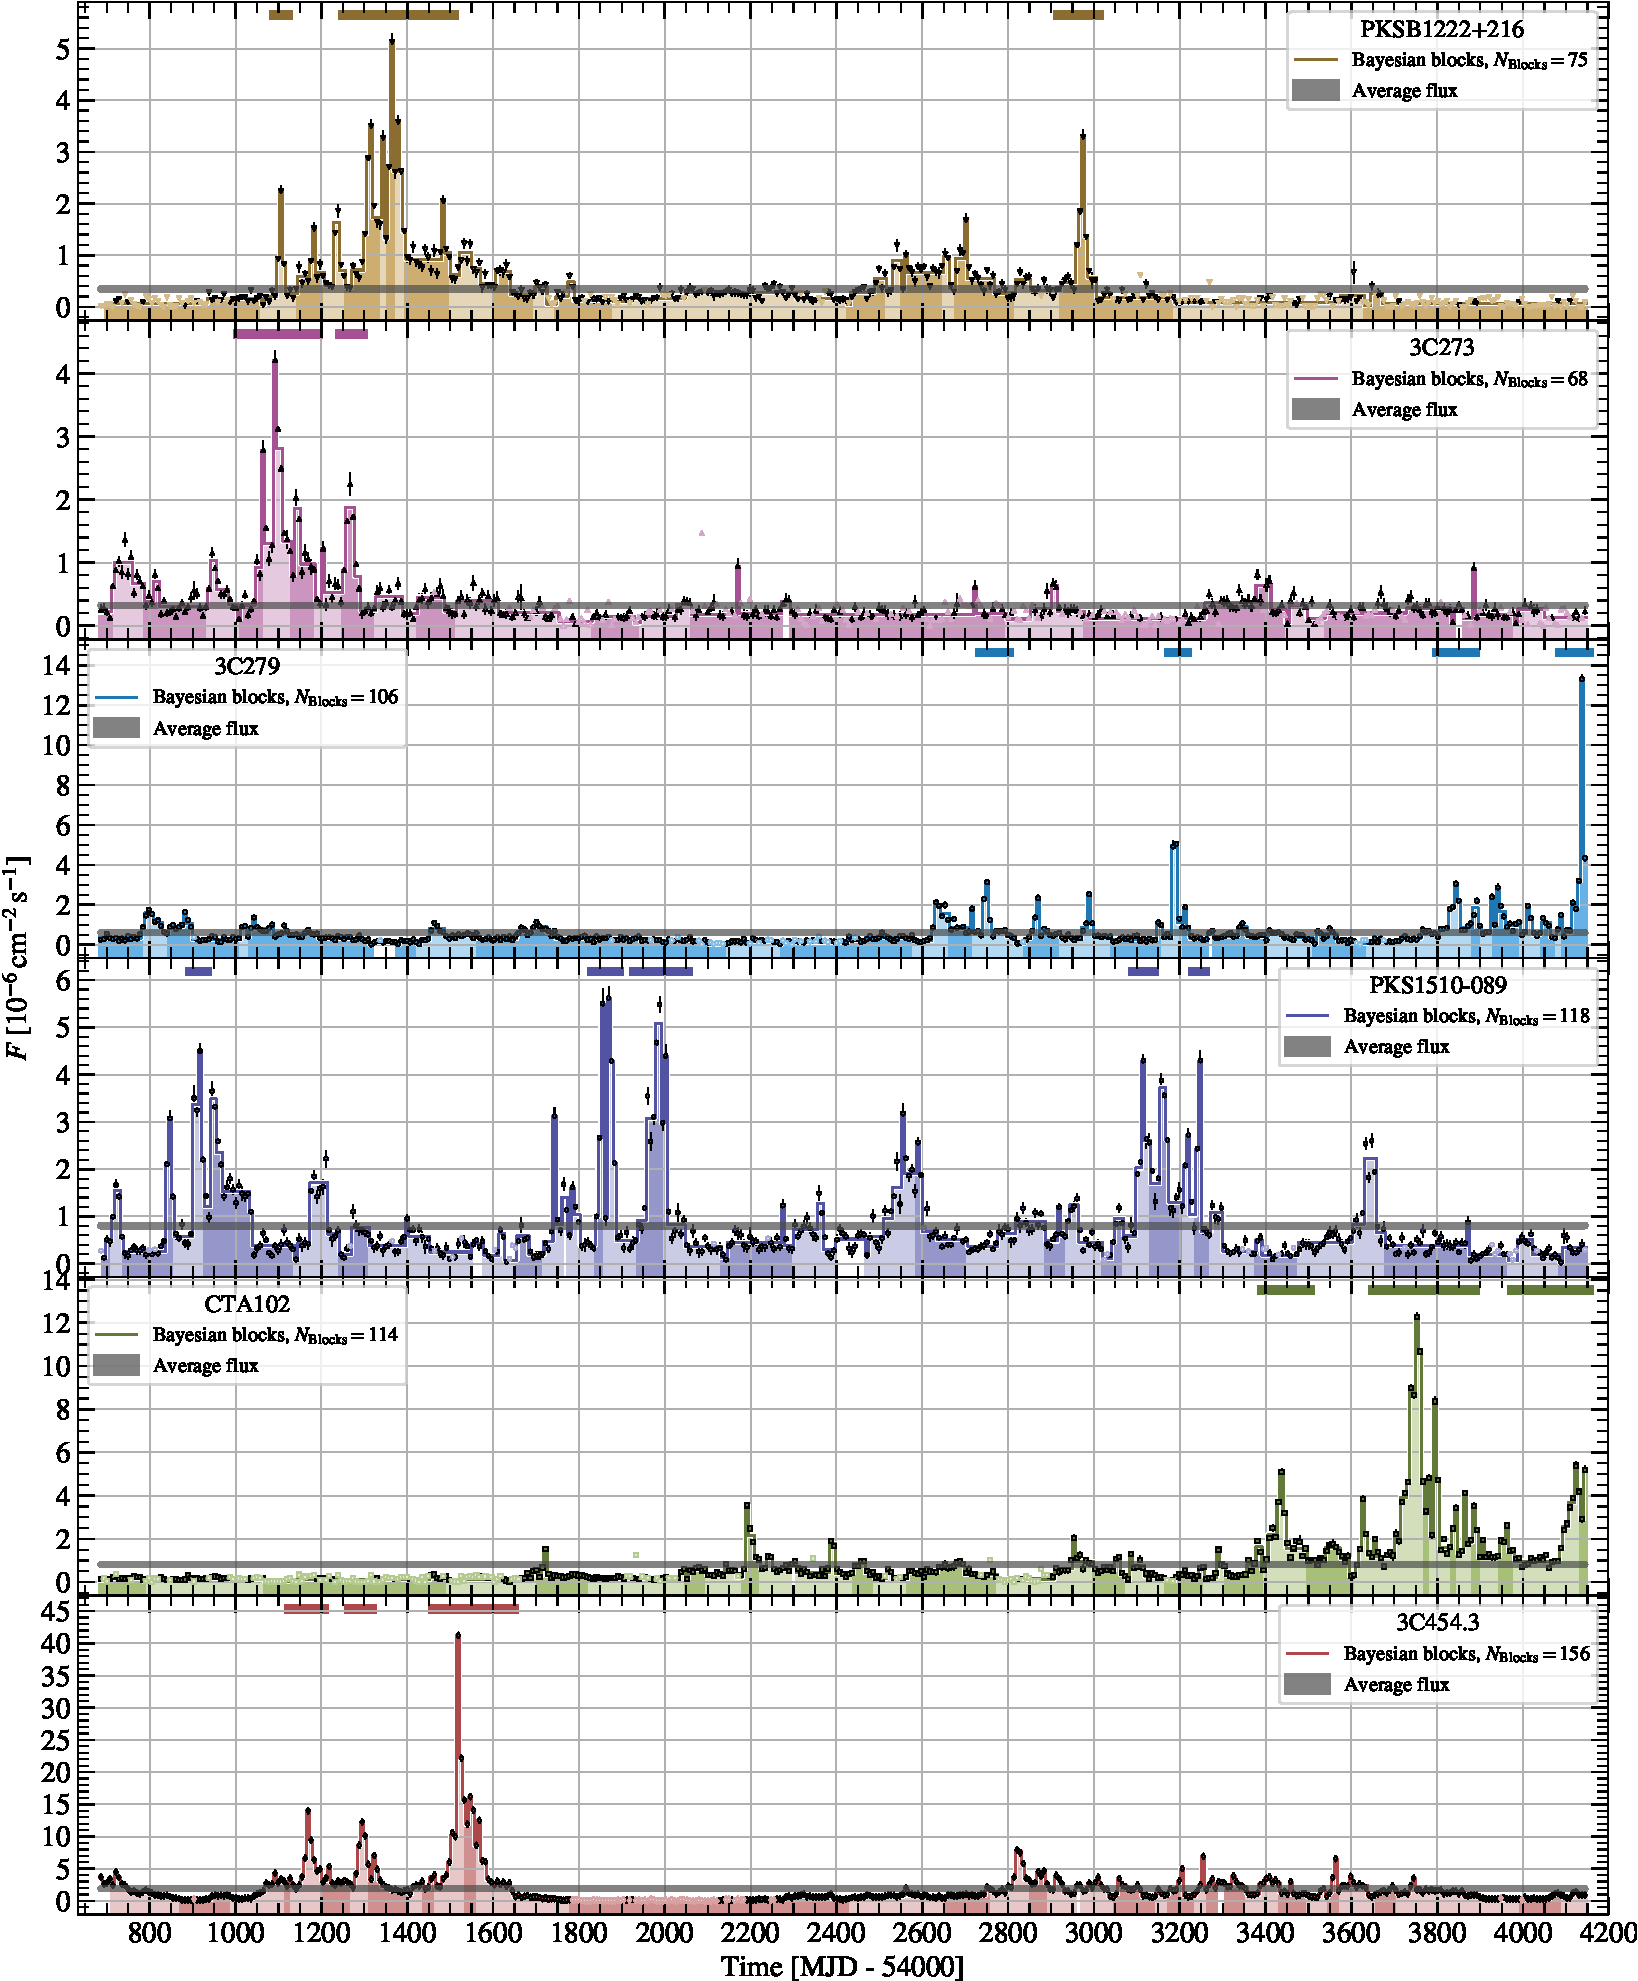
\includegraphics[width = .9\linewidth]{figures/lc_weekly_tsmin9.pdf}
    \caption{\gray light curves with weekly binning for the considered FSRQs. Open symbols denote upper limits at the $2\,\sigma$ confidence level. The orange lines show the BBs and the hatched regions represent the identified HOP groups. The green shaded regions denote the time intervals identified as bright flares for which we derive light curves with finer binning.}
    \label{fig:weekly}
\end{figure*}

There is no generally accepted consensus to determine the data points that belong to a flaring state and which characterize the quiescent level. \citet{2013MNRAS.430.1324N} suggests a simple definition that a flare is a continuous time interval associated with a flux peak in which the flux is larger than half the peak flux value. 
This definition is intuitive, however, it is unclear how to treat overlapping flares and identify flux peaks in an unbiased way. 
To mitigate these problems, we have implemented a one dimensional hill-climbing algorithm based on   HOP algorithm~\citep{1998ApJ...498..137E}.
The algorithm associates data points to their nearest neighbor weighted by flux.
We feed the BB representation of the light curve to the HOP algorithm and the resulting groups of data points are shown 
Fig.~\ref{fig:weekly} as left and right hatched areas. \todo{Jeff, do you want to provide some more details here?}
The combination of BBs and the HOP algorithm represents an unbiased way to split a light curve into groups of quiescent and flaring episodes; we will refer to one connected flare episode as a \emph{HOP group} of consecutive BBs.

We iteratively zoom in on time ranges with bright \gray activity by identifying HOP groups where one BB fulfills the condition $F_{BB} \geqslant F_\mathrm{max} =  5\times\overline{F}$ and including adjacent blocks within the group with $F_{BB} \geqslant F_\mathrm{min} = \overline{F}$. We prefer this minimum flux criterion over including the full HOP group as it might extend over long time ranges of a quiescent state.
Overlapping time ranges are combined into one time range and the ranges are extended by one time bin on either side.
For the identified time span, we re-optimize the spectral model of the ROI in the same way as described in Sec.~\ref{sec:roi} but without re-localizing the central FSRQ or adding new point sources. Subsequently, we calculate a light curve with finer binning and again select the time ranges of the highest \gray activity. We repeat this procedure twice, down to a binning equal to the Good Time Intervals (GTIs), of the \Fermi satellite, which correspond to one passage of the source through the field of view of the satellite during one $\sim$ 95 minute orbit.
The choices of time binnings and values for $F_\mathrm{max}$ and $F_\mathrm{min}$ are summarized in Tab.~\ref{tab:zoom} together with the number of identified high \gray activity states (which might consists of several flares as indicated by the HOP groups).
The values of the threshold fluxes $F_\mathrm{max}, F_\mathrm{min}$ is somewhat arbitrary and are a compromise between including as many flares as possible but keeping the overall number of flares manageable. Note, that the sole purpose of this exercise is to select the brightest flares for  further analysis. 
The resulting time ranges for the weekly light curves are plotted as green shaded areas in Fig.~\ref{fig:weekly}.
The intermittent daily light curves are provided in Fig.~\ref{fig:daily}.
Figure~\ref{fig:gti} shows the GTI (or orbital) light curves with exponential fits of flare profiles that we will discuss in Sec.~\ref{sec:results-local}. 
The source exposure can vary significantly between two adjacent orbits of the orbital light curve, as the satellite rocks between the celestial north and south pole in between orbits. 
This explains the large error bars on some of the time bins of the GTI light curves.

\begin{deluxetable}{cccc}
\tablewidth{1\linewidth}
\tablecaption{ \label{tab:zoom} Thresholds for BB fluxes in one HOP group to select time ranges of \gray activity together with selected time binning and number of selected time ranges.
}
\tablehead{Binning & $F_\mathrm{min}$ & $F_\mathrm{max}$ & $N_\mathrm{time~ranges}$}
\startdata
7 days & $\overline{F}$ & $5\times\overline{F}$ & 20\\
1 day & $\overline{F}$ & $\mathrm{max}(10^{-5}\,\mathrm{cm}^{-2}\,\mathrm{s}^{-1}, 1.5 \times \overline{F})$\tablenotemark{a} & 21\\
GTI & $\overline{F}$ & $2\times\overline{F},~\mathrm{TS} \geqslant 150$\tablenotemark{b} & 7\\
%Sub-GTI & -- & -- & --\\
\enddata
\tablenotetext{a}{We choose here the absolute flux (rather than the flux relative to the average) as a threshold in order to be consistent with our initial source selection. However, because of the high avergage flux of 3C454.3, we also include the max argument. If $F_\mathrm{max} = 1.5 \times \overline{F}$ we set $F_\mathrm{min} = 10^{-5}\,\mathrm{cm}^{-2}\,\mathrm{s}^{-1}$. }
\tablenotetext{b}{Motivated from the high $\mathrm{TS}$ found for the flare of 3C\,279~\citep{TheFermi-LAT:2016dss}, we also demand that at least one GTI of each HOP group is detected with $\mathrm{TS} \geqslant 150$ in order to ensure enough statistics to search for variability on time scales of minutes.}
\tablecomments{If no interval fulfills the $F_\mathrm{BB} \geqslant F_\mathrm{max}$ criterion for the weekly or daily light curves, we include the HOP group of the maximum flux if that flux exceeds $5\times10^{-6}\,\mathrm{cm}^{-2}\,\mathrm{s}^{-1}$, i.e., we change $F_\mathrm{max}$ to the maximum value $F_\mathrm{BB}$.}
\end{deluxetable}

In a last step, we derive light curves on sub-GTI time scales. 
The time bin size is calculated from the adaptive binning method of \citet{lott2012}, where we choose bins of constant flux uncertainty of $\sim20\,\%$. 
In this step, we use the space craft information in time steps of 1\,s instead of 30\,s. Additionally, we compute the effective area in 5 bins of the azimuthal spacecraft coordinates since on such short time scales the exposure dependence on the azimuth should not be averaged over.\footnote{See \url{https://fermi.gsfc.nasa.gov/ssc/data/analysis/scitools/help/gtltcube.txt}}
We discuss these light curves in Sec.~\ref{sec:sub-gti}.


%%% Daily light curves %%%%%%%%%
\begin{figure*}
    \centering
    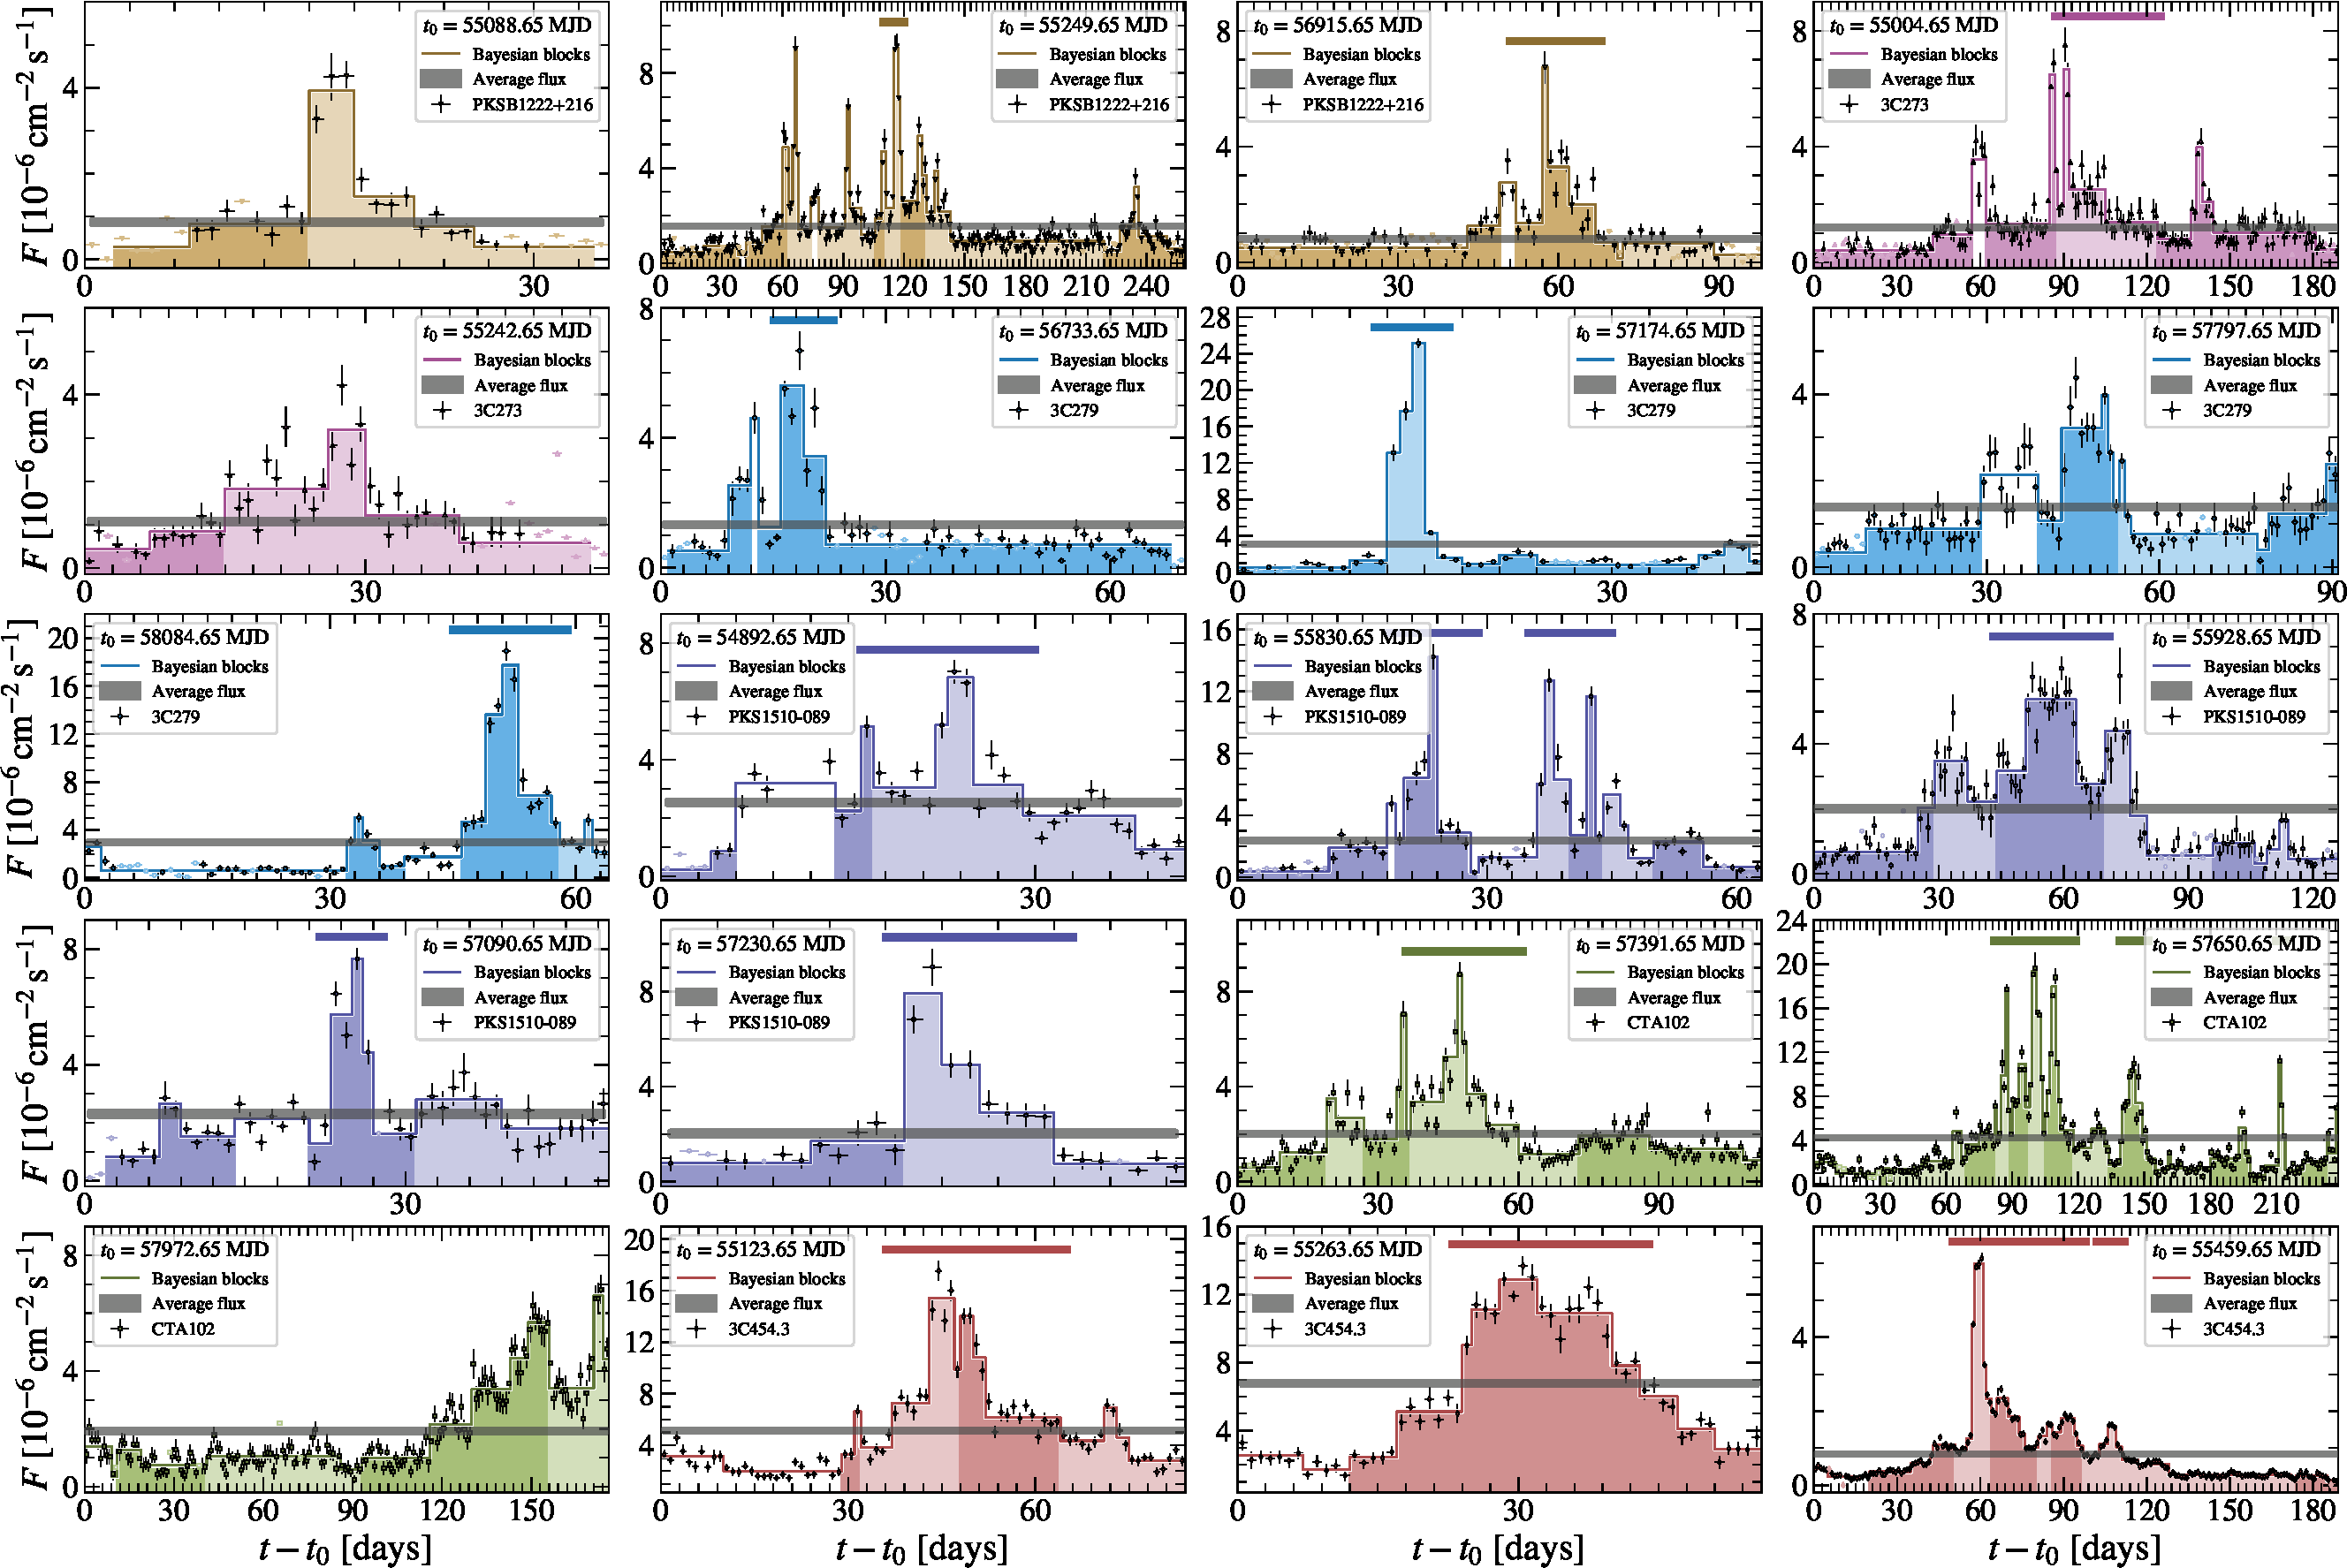
\includegraphics[width = .99\linewidth]{figures/lc_daily_tsmin9.pdf}
    \caption{\label{fig:daily} Light curves with daily binning for the selected time ranges (green shaded regions in Fig.~\ref{fig:weekly}). Symbols and lines are the same as in Fig.~\ref{fig:weekly}. 
    As stated in Tab.~\ref{tab:zoom}, if all BB fluxes fail the criterion $F_{BB} \gtrsim \mathrm{max}(10^{-5}\,\mathrm{cm}^{-2}\,\mathrm{s}^{-1}, 1.5 \bar{F})$, we include the HOP group with the maximum flux of the interval if that flux is above $5\times 10^{-6}\,\mathrm{cm}^{-2}\,\mathrm{s}^{-1}$. This is the case, e.g., for last two intervals of PKSB1222+216 and the first interval of 3C273 (last three panels of the top row).}
\end{figure*}
%%%%%%%%%%%%%%%%%%%%%%%%%%%%%%%%

\section{Results for global light curve properties}
\label{sec:results-global}
We first present results derived from the weekly \gray light curves spanning the full 9.5\,year time range, which we refer to \emph{global light curve properties}, before deriving results from the local light curves on GTI and sub-GTI time scales in Sec.~\ref{sec:results-local}.

From the weekly light curves in Fig.~\ref{fig:weekly} it is evident that the FSRQs show strong flares that exceed the average flux by a factor of a few, while the quiescent level is relatively stable. 
Such behavior is typical for FSRQs~\citet{} and we 
further quantify it by calculating the flux distribution, $dN/dF$, of the weekly fluxes for bins with $\mathrm{TS} > 9$ and $F_i > \sigma_i$. 
The results are shown in Fig.~\ref{fig:fluxpdf}. The flux bins are chosen according to the algorithm of~\citet{knuth2006} and the error bars are calculated under the assumption that the observed weekly fluxes, $F_i$, $i = 1,\ldots,N$, are Gaussian distributed numbers with standard deviation equal to the measurement uncertainty $\sigma_i$.\footnote{
With this assumption, the uncertainty to find $x$ entries in the $j$-th flux bin of width $\Delta F_j = F_{\mathrm{hi},j} - F_{\mathrm{lo},j}$ is given by the sum of Bernoulli probabilities $p_{ij}$, $\sum_{i = 1}^N p_{ij}(1-p_{ij})$, where $p_{ij} =  \left[\mathrm{erf}\left((F_{\mathrm{hi},j} - F_i) / \sqrt{2\sigma_i^2}\right) - \mathrm{erf}\left(((F_{\mathrm{lo},j} - F_i) / \sqrt{2\sigma_i^2}\right)\right]/2$, and $\mathrm{erf}$ is the error function.
}
We fit the flux distribution with a smoothly broken power law (BPL) of the form 
\begin{equation}
    \frac{dN}{dF} = N_0 \left( \frac{F}{F_0}\right)^{\alpha_\mathrm{low}}
        \left( 1 - \left(\frac{F}{F_\mathrm{br}}\right)^s \right)^{\frac{\alpha_\mathrm{high} - \alpha_\mathrm{low}}{s}},
        \label{eq:dndf}
\end{equation}
with the smoothing factor $s$ fixed to 3. 
The results of a $\chi^2$ minimazation are summarized in Tab.~\ref{tab:global}.
Generally, below the break flux $F_\mathrm{br}$, the flux distribution is flat, $\alpha_\mathrm{low}\sim 0$.
Above $F_\mathrm{br}$ which lies between $\sim2\times10^{-7}$ and $\sim2\times10^{-6}\,\mathrm{cm}^{-2}\mathrm{s}^{-1}$, $dN/dF$ declines exponentially with power-law indices $\alpha_\mathrm{high} \lesssim -2.2$, making the brightest flares rare events.
Furthermore, it is clear that the flux distribution is very different from Gaussian behavior. 

\begin{figure}
    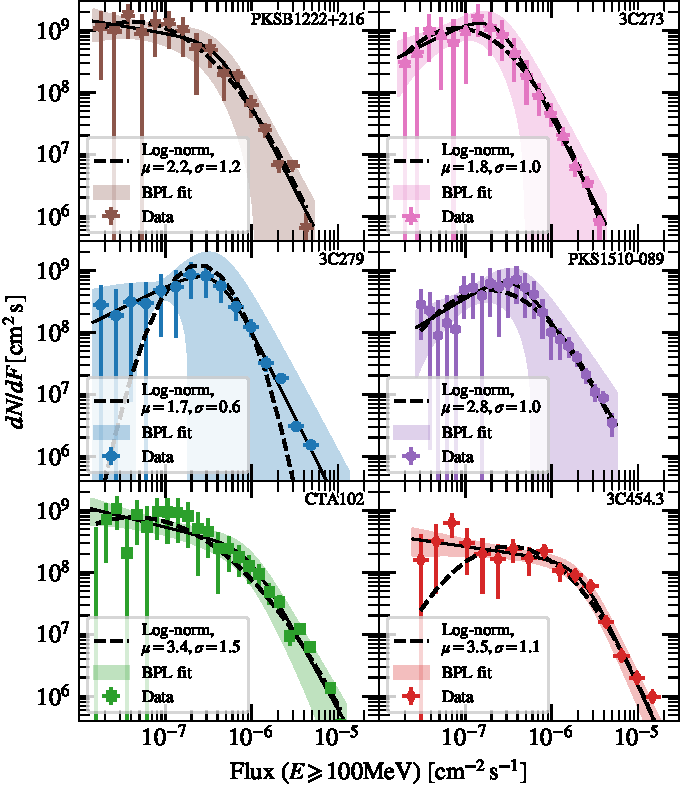
\includegraphics[width = .99\linewidth]{figures/fluxdist_weekly_tsmin9.pdf}
    \caption{\label{fig:fluxpdf} Distribution of the fluxes of the weekly 9.5 year \gray light curves. The BPL fit is shown as a black line with $1\,\sigma$ uncertainties shown as shaded bands. \todo{fit with log normal distribution?}}
\end{figure}

We further characterize the global \gray light curves in terms of their PSD,
which usually can be described with simple power laws in frequency,  $\mathrm{PSD} \propto 1 / \nu^\beta$~\citep{}.
An analysis of the first 11~months of LAT data from 106 blazars revealed that 
these objects have $\beta$ values between 1 and 2, the intermittent regime between flicker noise ($\beta = 1$) and Brownian motion ($\beta = 2)$~\citep{2010ApJ...722..520A}. 
In addition to the noise behavior, 
we further use the derived PSDs in Sec.~\ref{} to simulate \gray light curves in order to calculate the significance of a correlation between radio and \gray emission. 

The best-fit PSDs are estimated from the periodograms and simulated light curves following the method described in detail in \citet{2014MNRAS.445..437M} and \citet{2013MNRAS.433..907E} and summarized briefly below.
The observed periodograms $P(\nu)$ as a function of frequency $\nu$ are calculated from the absolute square of the Fourier transformation of the light curve (Eq.~(3) of \citealt{2014MNRAS.445..437M}) including all 
data points detected with $\mathrm{TS} \geqslant 9$ and performing a linear interpolation between gaps in the light curve. Since we are using weekly binned light curves and bright FSRQs the gaps are small and at most 6 consecutive data points long (42\,days) in the case of PKS\,B1222+216. The number of non-detected bins is less than $\sim13\,\%$ for all sources.
The interpolation is done in time steps of $\Delta t=0.7\,$days and 
 re-binned into bins of lengths of 7 days by taking the geometrical mean of the flux.
In contrast to~\citet{2014MNRAS.445..437M}, we do not apply a window function (see the discussion below). 

We simulate light curves using the method of \citet{1995A&A...300..707T} with a time steps equal to 0.7\,days for power-law PSDs with values $0 \leqslant \beta \leqslant 3$ in steps of $\Delta\beta = 0.05$. For each $\beta$ value 100 light curves are generated, each one a 100 times longer than the actual observation to account for possible red-noise leakage. Splitting the simulated light curves (without overlap) leaves us with $10^4$ realizations. 
The light curves are then re-binned into 7-day light curves through averaging. The same observational gaps and interpolation as in the observed light curves are applied. 
The periodograms are then calculated for light curve in the same way for the observed light curve.
To fix the normalization of the PSD model, \citet{2014MNRAS.445..437M} suggest variance matching, i.e., they rescale the simulated flux data points with a factor $A^{-1}$, where $A^2 = \sigma_\mathrm{sim}^2 / (\sigma_\mathrm{obs}^2 - \bar{\sigma_i^2})$, with $\sigma_\mathrm{sim}^2$ ($\sigma_\mathrm{data}^2$) the variance of the simulated (observed) light curve and $\bar{\sigma_i^2}$ the variance of the observational noise.
For the \gray light curves, we choose to follow \citet{2013MNRAS.433..907E} instead and iteratively match the probability distribution of the simulated fluxes to the observed ones, given by the $dN/dF$ distrutions shown in Fig.~\ref{fig:fluxpdf}. 
The reason is that the algorithm of \citet{1995A&A...300..707T} produces light curves with Gaussian distributed fluxes, which is clearly not the case at \gray energies.\footnote{Furthermore, the variance matching relies on Parseval's theorem from which it follows that the light curve variance is equal to the integrated PSD. However, Parseval's theorem is only valid for square-integrable functions, i.e. $\beta \geqslant 2$ and thus not strictly applicable for smaller values of $\beta$ commonly observed at \gray energies.}
In a final step, we add uncertainties to the light curves by randomly drawing with replacement from the observed uncertainties $\sigma_i$ and adding a Gaussian random number $\mathcal{N}(0,\sigma_i)$ to the simulated flux values.

The peridograms of the observed and simulated light curves, ${P}_\mathrm{obs}$ and ${P}_\mathrm{sim}$, are averaged in logarithmic bins~\citep{1993MNRAS.261..612P} and compared by means of a $\chi^2$ test~\citep{2014MNRAS.445..437M},
\begin{equation}
    \chi^2(\beta) = \sum_{\nu_\mathrm{min}}^{\nu_\mathrm{max}}\frac{(P_\mathrm{obs}(\nu) - \overline{P}_\mathrm{sim}(\nu,\beta))^2}{\Delta\overline{P}_\mathrm{sim}(\nu,\beta)^2},\label{eq:chi2psd}
\end{equation}
where $\Delta\overline{P}_\mathrm{sim}(\nu)^2$ is the variance of the simulated light curves.
The averaged periodograms of the simulated light curves and the observed ones are shown in Fig.~\ref{fig:periodograms} and the best fit average periodogram is shown as a thick solid line. 
The quality of the the best-fit value $\hat\beta$ with corresponding minimum $\chi^2$ value $\hat\chi^2\equiv\chi^2(\hat\beta)$, is evaluated from the light curves simulated with $\beta = \hat\beta$ in the following way. We form the distributions of simulated $\chi^2$ values, $\chi^2_\mathrm{sim}$, by replacing $P_\mathrm{obs}(\nu)$ with $P_\mathrm{sim}(\nu,\beta)$ in Eq.~(\ref{eq:chi2psd}),
\begin{equation}
    \chi^2_\mathrm{sim}(\beta,\beta') = \sum_{\nu_\mathrm{min}}^{\nu_\mathrm{max}}\frac{(P_\mathrm{sim}(\nu,\beta) - \overline{P}_\mathrm{sim}(\nu,\beta'))^2}{\Delta\overline{P}_\mathrm{sim}(\nu,\beta')^2},\label{eq:chi2psd_sim}
\end{equation}
and calculate the $p$-value as the  fraction of simulations that result in $\chi^2_\mathrm{sim}(\hat\beta,\hat\beta) > \hat\chi^2$.
The confidence interval for $\hat\beta$ is derived by determining the $\Delta\chi^2_\mathrm{sim}(\hat{\beta},\beta)$ value from simulations such that 95\,\% of the time the simulated (true) $\beta$ value is contained within $\Delta\chi^2$. 
The same $\Delta\chi^2$ value is then applied to the observed $\chi^2$ curve.
The results of our PSD analysis are summarized in Tab.~\ref{tab:global} where we also report the value of $\beta$ obtained from a linear regression in log-log space. 
In general, the periodograms are well fit by our method, as indicated by the $p$-values and observed in Fig.~\ref{fig:periodograms}. 
The only exception is 3C\,279 where only 2 of the $10^4$ simulated light curves result in a $\chi^2_\mathrm{sim}(\hat\beta,\hat\beta) > \hat\chi^2$.
The steep $\chi^2$ curve for this source also explains the small error bars on the reconstructed value of $\beta$.
The reason might be a more complex underlying PSD or the specific 7 day binning we have chosen here. 
\todo{mention bumps / QPOs?}

\begin{figure*}
    \centering
    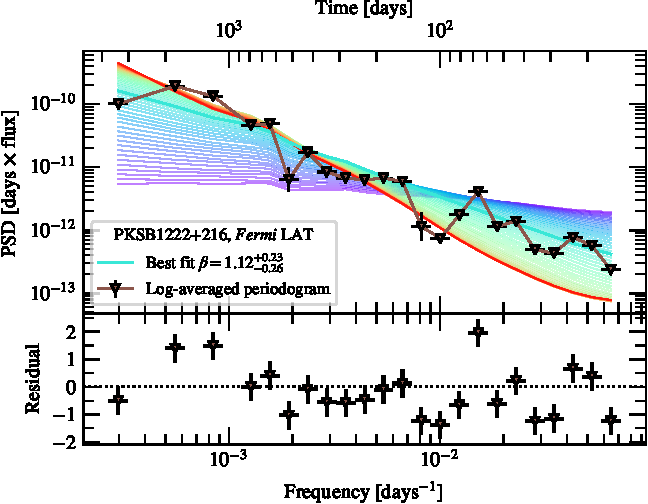
\includegraphics[width = 0.32\linewidth]{figures/periodogram_fermi_PKSB1222+216_Nsim_100Next_100Sim_addunc_data_rescale_EM13_usegap_1_PSD_window_none_detrend_none_norm_var_20.pdf}
    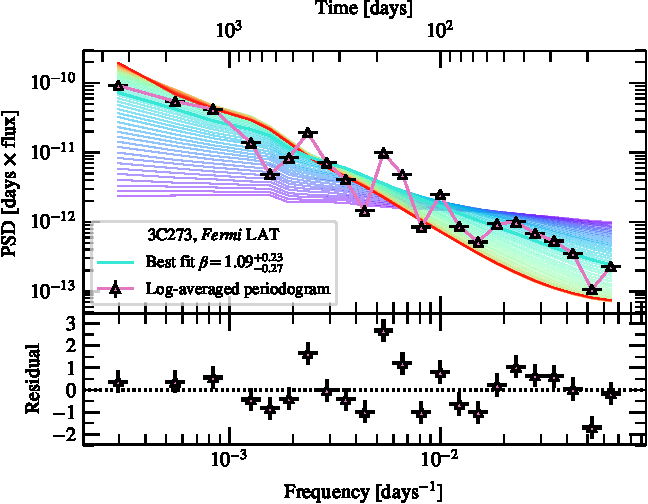
\includegraphics[width = 0.32\linewidth]{figures/periodogram_fermi_3C273_Nsim_100Next_100Sim_addunc_data_rescale_EM13_usegap_1_PSD_window_none_detrend_none_norm_var_20.pdf}
    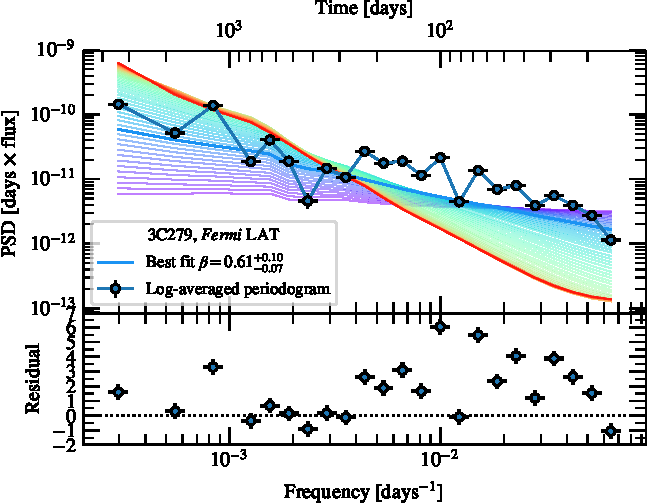
\includegraphics[width = 0.32\linewidth]{figures/periodogram_fermi_3C279_Nsim_100Next_100Sim_addunc_data_rescale_EM13_usegap_1_PSD_window_none_detrend_none_norm_var_20.pdf}
    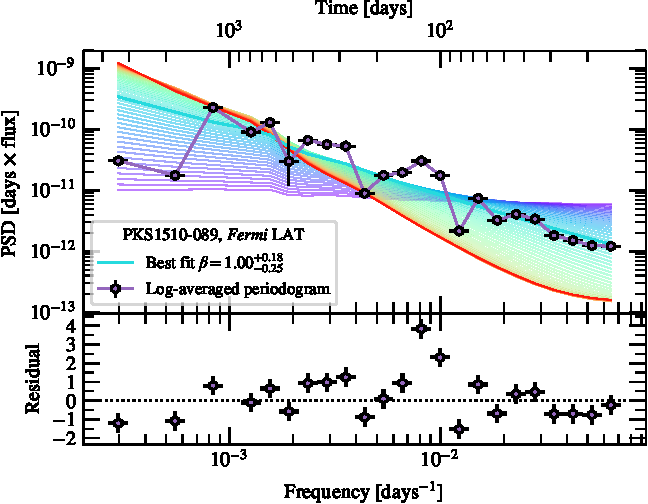
\includegraphics[width = 0.32\linewidth]{figures/periodogram_fermi_PKS1510-089_Nsim_100Next_100Sim_addunc_data_rescale_EM13_usegap_1_PSD_window_none_detrend_none_norm_var_20.pdf}
    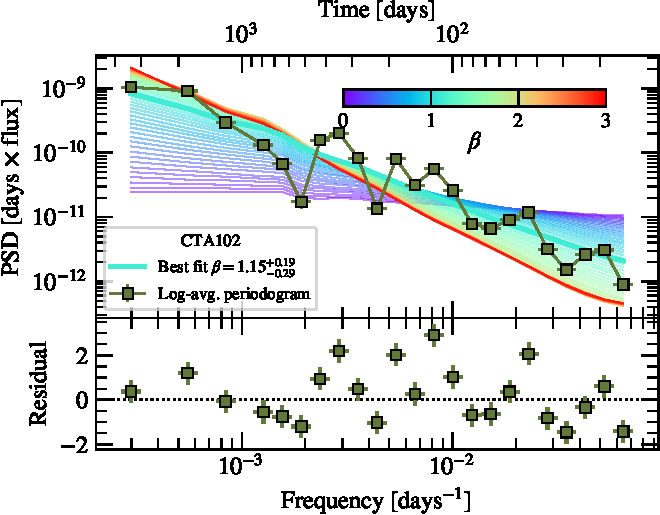
\includegraphics[width = 0.32\linewidth]{figures/periodogram_fermi_CTA102_Nsim_100Next_100Sim_addunc_data_rescale_EM13_usegap_1_PSD_window_none_detrend_none_norm_var_20.pdf}
    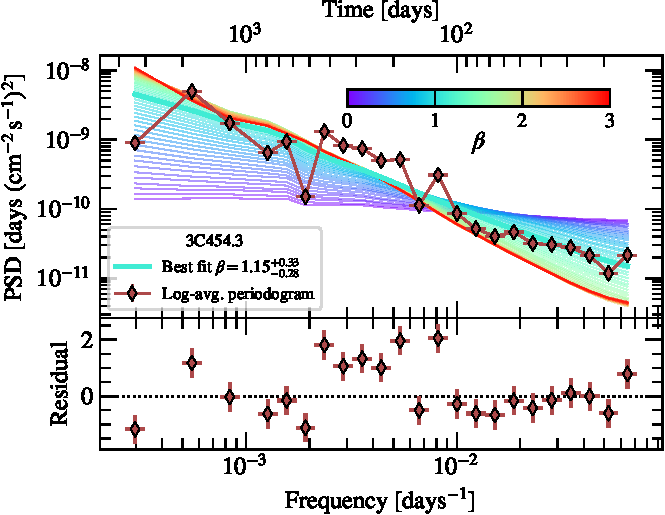
\includegraphics[width = 0.32\linewidth]{figures/periodogram_fermi_3C454p3_Nsim_100Next_100Sim_addunc_data_rescale_EM13_usegap_1_PSD_window_none_detrend_none_norm_var_20.pdf}
    \caption{Periodograms of the observed (markers) and simulated light curves (colored lines). The simulated periodograms follow power-law PSDs between $\beta = 0$ (purple line) to $\beta = 3$ (red line) in steps of $\Delta\beta = 0.05$. The bottom panels show the residuals with respect to the best fit which is indicated in the legend and as a thick solid line in the upper panels.}
    \label{fig:periodograms}
\end{figure*}


\begin{deluxetable*}{lcccccc}
\tablewidth{0pt}
\tablecaption{ \label{tab:global}Global \gray light curve properties.}
\tablehead{Source name & $\alpha_\mathrm{low}$ & $\alpha_\mathrm{high}$ & $F_\mathrm{br} [10^{-6}\mathrm{cm}^{-2}\mathrm{s}^{-1}]$ 
& $\beta_\mathrm{slope}$ & $\hat\beta$ & $p$-value
}
\startdata
PKSB1222+216 & $-0.24^{+0.41}_{-0.27}$ & $-2.70^{+0.33}_{-0.43}$ & $0.42^{+0.28}_{0.15}$ &  1.23 & $1.12^{+0.21}_{-0.26}$ & 0.423 \\
3C273 & $0.70^{+0.40}_{-0.54}$ & $-2.77^{+0.24}_{-0.27}$ & $0.23^{+0.07}_{0.07}$  & 1.14 & $1.09^{+0.24}_{-0.27}$ & 0.330 \\
3C279 & $0.68^{+0.27}_{-0.40}$ & $-2.80^{+0.21}_{-0.23}$ & $0.40^{+0.10}_{0.10}$ & 0.67 & $0.61^{+0.10}_{-0.07}$ & $2\times10^{-4}$ \\
PKS1510-089 & $0.84^{+0.72}_{-0.48}$ & $-2.21^{+0.23}_{-0.26}$ & $0.40^{+0.16}_{0.12}$ & 0.88 & $1.00^{+0.18}_{-0.25}$ & 0.129 \\
CTA102 & $-0.35^{+0.22}_{-0.18}$ & $-2.50^{+0.16}_{-0.19}$ & $0.90^{+0.38}_{0.26}$ & 1.21 & $1.18^{+0.16}_{-0.32}$ & 0.138 \\
3C454.3 & $-0.20^{+0.17}_{-0.13}$ & $-3.00^{+0.13}_{-0.14}$ & $2.19^{+0.39}_{0.32}$ & 1.05 & $1.15^{+0.32}_{-0.28}$ & 0.274 \\
\enddata
{
\tablecomments{Columns 2-4 indicate the best-fit values for the BPL fit [Eq.~(\ref{eq:dndf})] to the $dN/dF$ distributions, whereas columns 5-7 show the best-fit results for the PSD. $\beta_\mathrm{slope}$ gives the result for a linear regression of the periodograms and $\hat\beta$ is the best-fit value of the $\chi^2$ minimization with corresponding $p$-value. The interval around $\hat\beta$ is at 95\,\% confidence.}
}
\end{deluxetable*}

\section{Results for local light curve properties}
\label{sec:results-local}
%\subsection{Local light curve properties}
%\label{sec:hop-fit}

We proceed with deriving local properties of the \gray flares from the light curves with one bin per GTI that are shown in Fig.~\ref{fig:gti}.

%%% GTI light curves %%%%%%%%%
\begin{figure*}
    \centering
    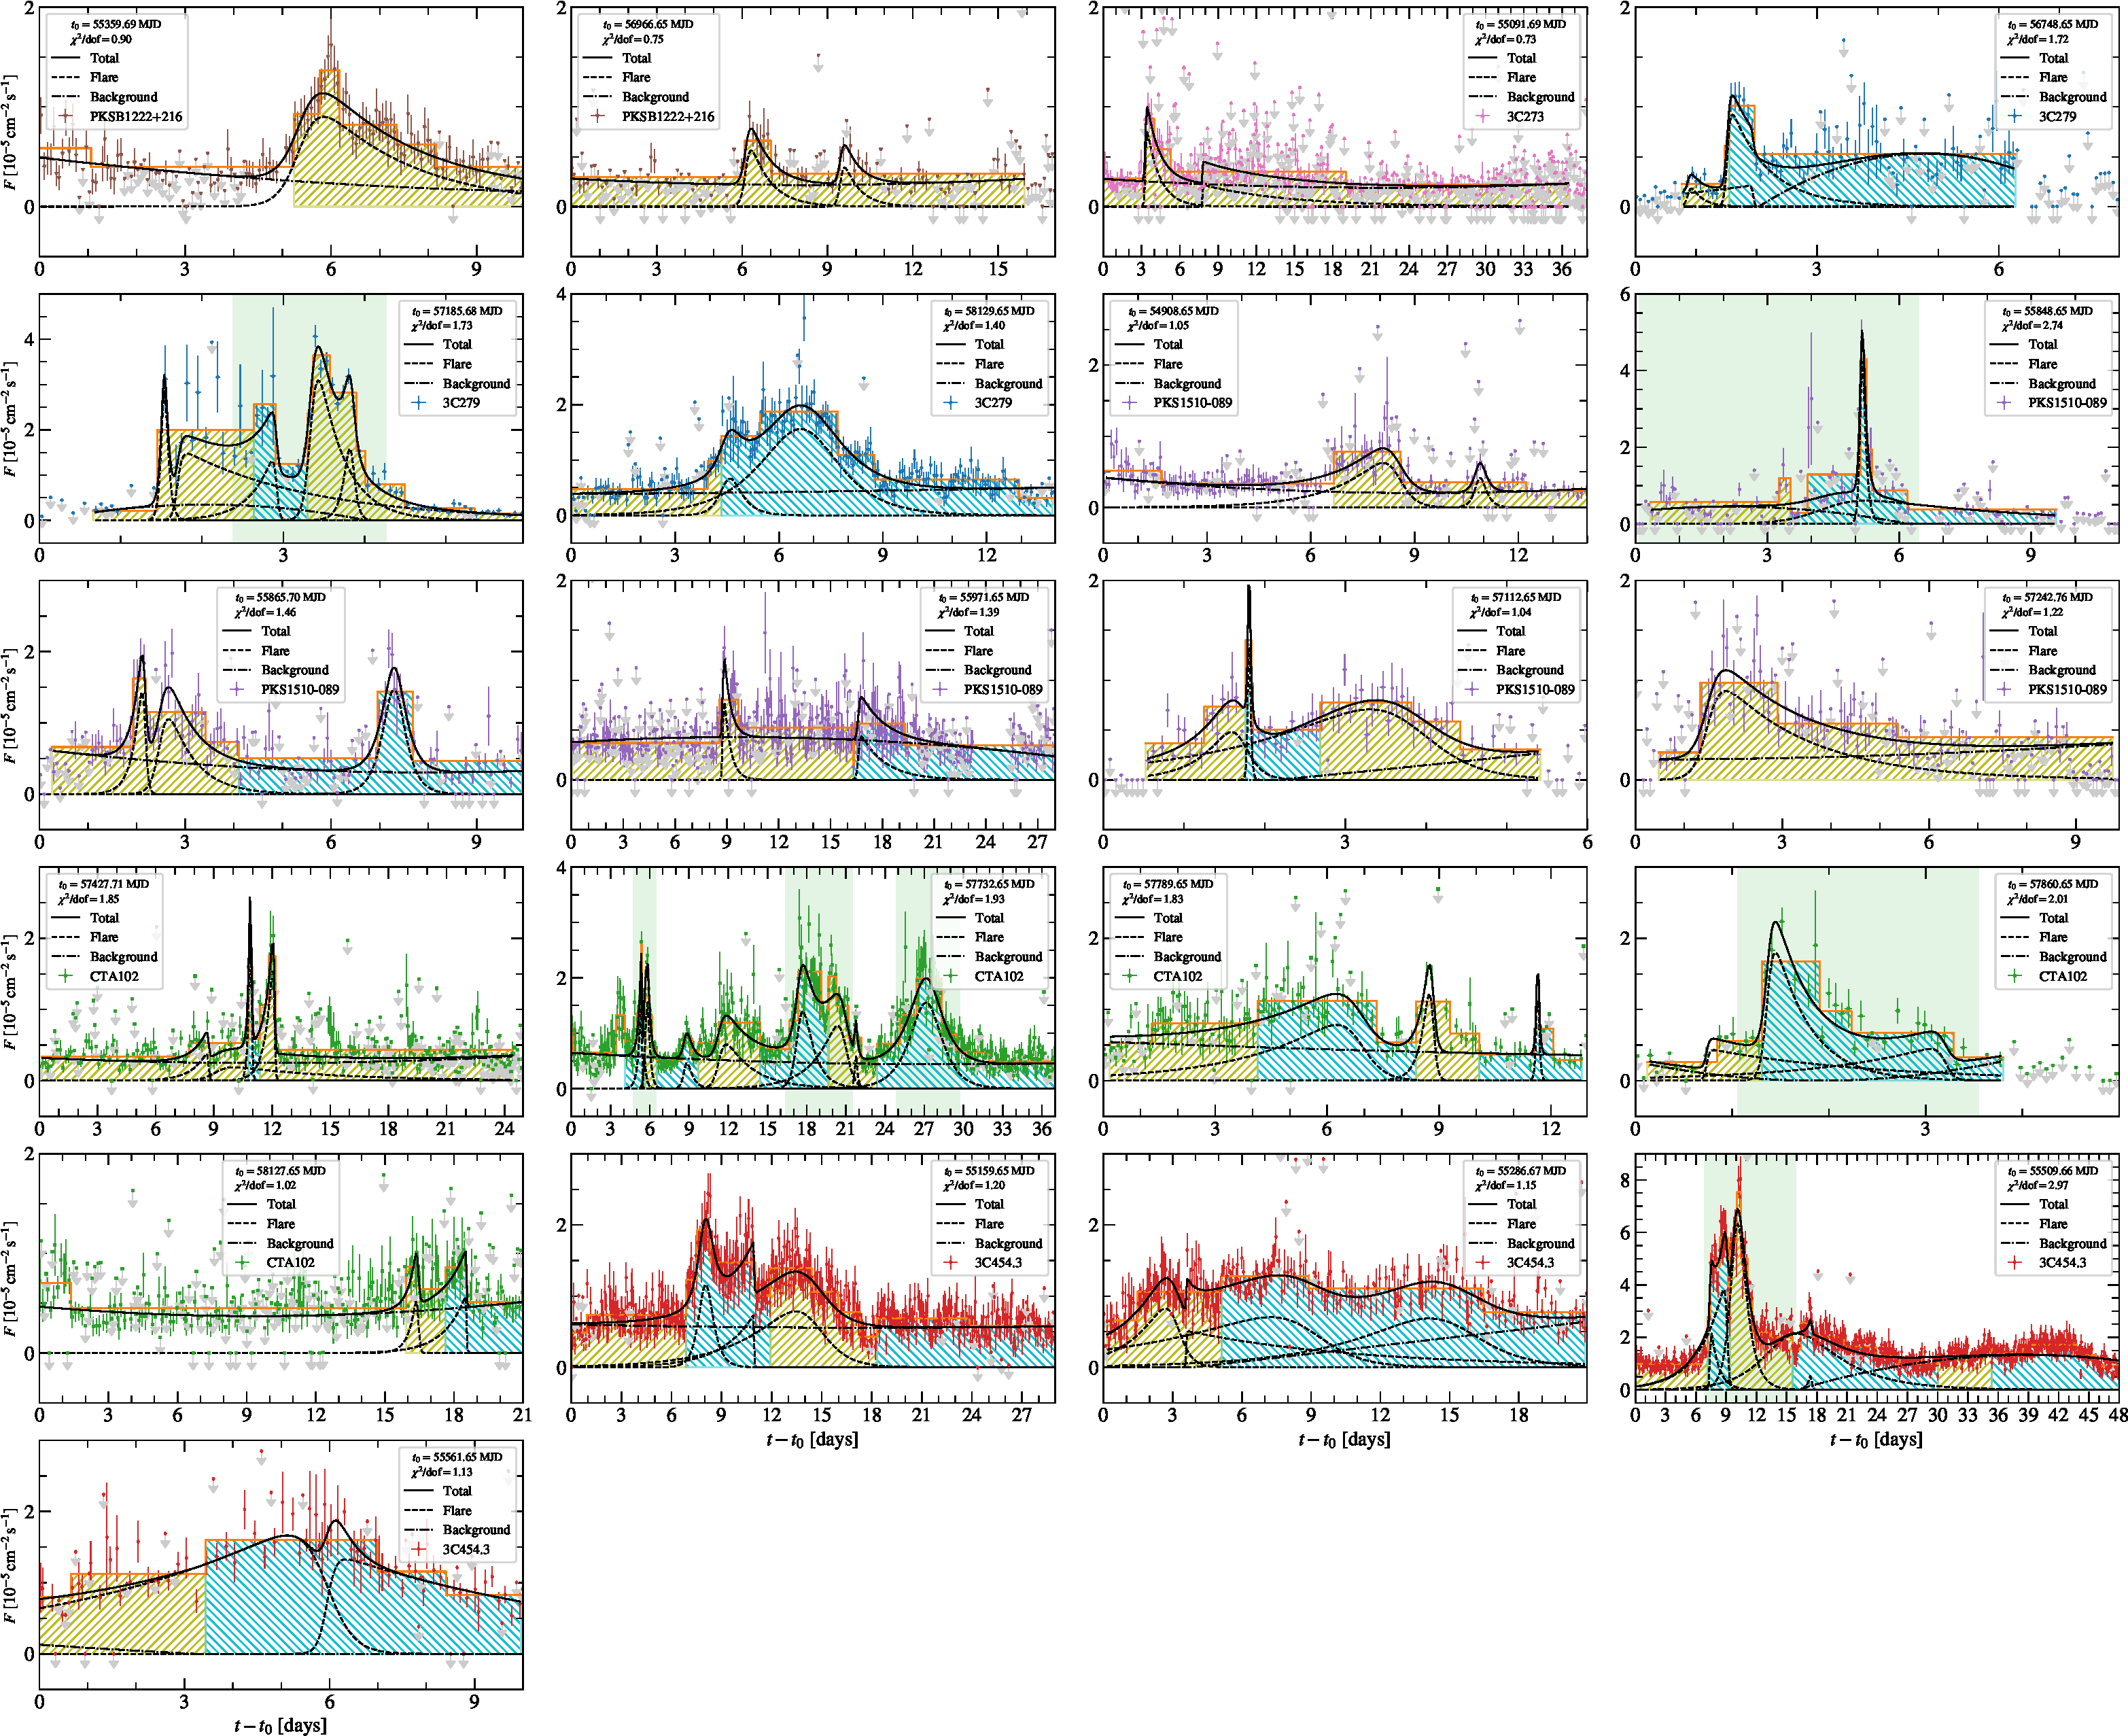
\includegraphics[width = .99\linewidth]{figures/lcfithop_orbit_all_maxiter2_fsys0p00_addcomp0_comb.pdf}
    \caption{ Light curves with one bin per GTI for the selected time ranges (green shaded regions in Fig.~\ref{fig:daily}). Solid black and dashed lines show fits to the light curve with exponential flare profiles discussed in Sec.~\ref{sec:results-local}. Other symbols and lines are the same as in Fig.~\ref{fig:weekly} and ~\ref{fig:daily}.
    \todo{blue colors are missing!}
    }
    \label{fig:gti}
\end{figure*}
%%%%%%%%%%%%%%%%%%%%%%%%%%%%%%

To assess the time profile of the flares,
we fit each HOP group $i$ with a $\chi^2$ minimization as a sum of exponential profiles, 
\begin{eqnarray}
    F_{\mathrm{flare},i}(t) &=& 
    \sum\limits_{j = 1}^{N_i} F_{0,ij}\nonumber\\
    &\times&\left[\exp\left(\frac{t - t_{0,ij}}{\tau_{\mathrm{rise},ij}}\right) + \exp
    \left(\frac{t_{0,ij} - t}{\tau_{\mathrm{decay},ij}}\right)\right]^{-1}\!\!\!,
    \label{eq:flareHOP}
\end{eqnarray}
where $t_{0,j}$ are the flare peak times, and $\tau_{\mathrm{rise},ij}$, $\tau_{\mathrm{decay},ij}$ are the flare rise and decay times, respectively.
All light curve points are included that fulfill $\mathrm{TS}\geqslant9$ and $F_i \geqslant 3\sigma_i/2 $.
The number of flare profiles per HOP shed, $N_i$, is either 1 or 2 and determined during the fit using the Bayesian information criterion (BIC), defined as $\mathrm{BIC} = n_\mathrm{par}\ln(n) + \chi^2$, where $n_\mathrm{par}$ is the number of fit paramteres ($n_\mathrm{par} = 4$ for $N_i = 1$), $n$ is the number of data points within one HOP group $i$. Two flare profiles are selected if the difference between the two BIC values is $\Delta\mathrm{BIC} = \mathrm{BIC}(N_i = 2) - \mathrm{BIC}(N_i = 1) < 0$.
The reason for allowing $N_i > 1$ is that the flare profile in Eq.~(\ref{eq:flareHOP}) does not capture long-lasting plateaus of a flare present in multiple flares in Fig.~\ref{fig:gti} (see, e.g., all flares of 3C\,279 or the panel with a flare of 3C\,454.3 starting at 55551.65\,MJD).

After each HOP group is fitted individually and $N_i$ is determined, 
we re-fit the entire light curve, which consists of $N_\mathrm{HOP}$ groups, with the function 
\begin{equation}
    F_\mathrm{flare}(t) = \sum\limits_{i = 1}^{N_\mathrm{HOP}}F_{\mathrm{flare},i}(t) + F_\mathrm{bkg}(t),
\end{equation}
where $F_\mathrm{bkg}(t)$ is a order-2 polynomial to describe a slow  varying background.
The fit results are shown as black solid lines in Fig.~\ref{fig:gti}.
In general, the $\chi^2$ values divided by the degrees of freedom (dof) are between 1 and 2 (see the legends in Fig.~\ref{fig:gti}). Given the large values of dof, the fit qualities are usually poor. This is not unexpected, as we only allow up to two flare profiles per HOP group and not arbitrary functions. Already with this choice, there are probably some spurious flares identified, see, e.g., the second flare profile in the first PKS\,1510-089 flare (starting at 54908.65MJD). 
Nevertheless, the overall light curve evolution is well captured, which allows us to describe the local flare properties from the ensembles of flare profiles, keeping the above caveats in mind. 

We show the distribution of rise and decay times in the histograms of Fig.~\ref{fig:times-hist} for flares with a time integrated flux $>10^{-7}\,\mathrm{cm}^{-2}$. 
Remarkably, all sources show values of either $\tau_\mathrm{rise}$ or $\tau_\mathrm{decay}$ or both that are below the horizon crossing time scale of the central super massive black hole in the observer's frame, $t_g = r_g / c$, with $r_g = 2 G M_\bullet / c^2 $ the gravitational radius, $G$ the gravitational constant, black hole mass $M_\bullet$ (taken from Tab.~\ref{tab:src-select}), and $c$ the speed of light.
Most flares rise and decay within 2 hours or less. 
\begin{figure}
    \centering
    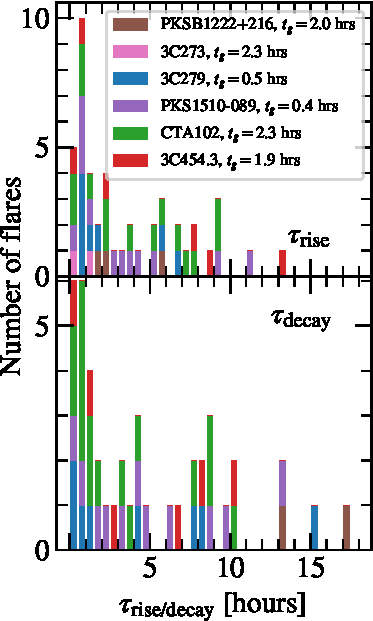
\includegraphics[width = .8\linewidth]{figures/lcfithop_results_tdtrhist_maxiter2_fsys0p00_addcomp0_orbit.pdf}
    \caption{Stacked bar graphs for  rise (top) and decay times (bottom) for the individual flares fitted in Fig.~\ref{fig:gti}. The legend gives the horizon crossing time scales $t_g$ in the observer's frame.}
    \label{fig:times-hist}
\end{figure}

From the rise and decay times, we can calculate the flare asymmetry as
\begin{equation}
    A = \frac{\tau_\mathrm{rise}-\tau_\mathrm{decay}}
    {\tau_\mathrm{rise}+\tau_\mathrm{decay}},
\end{equation}
so that $A < 0$ for fast-rise-exponential-decay (FRED) type flares, as expected from an injection of energetic particles that subsequently cool through radiative processes such as inverse Compton scattering or synchrotron emission.
The asymmtry is shown versus integrated flux, the peak flux, and the flare duration $T_{90}$, defined in the time around the flare peak that contains 90\,\% of the integrated flux, in Fig.~\ref{fig:asym}.
The peak flux for each flare of each HOP group is derived from the maximum of  Eq.~(\ref{eq:flareHOP}) with respect to time (suppressing indeces),
\begin{equation}
    F_{\mathrm{peak}} = \frac{F_{0} \tau_\mathrm{rise}}{\tau_\mathrm{rise} + \tau_\mathrm{decay}}\exp\left(\ln\left(\frac{\tau_\mathrm{decay}}{\tau_\mathrm{rise}}\right)\frac{\tau_\mathrm{decay}}{\tau_\mathrm{rise} + \tau_\mathrm{decay}}\right)
\end{equation}
The error bars on the peak flux and asymmetry are derived from standard Gaussian error propagation from the fit uncertainties.
\begin{figure*}
    \centering
    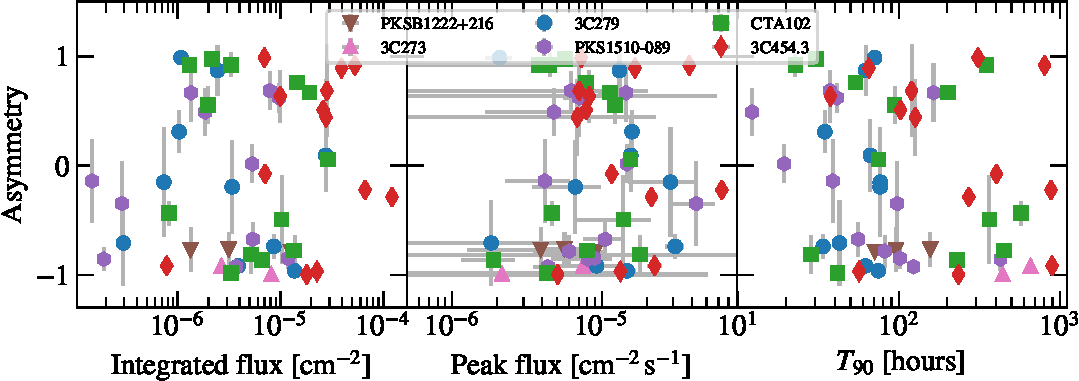
\includegraphics[width = .8\linewidth]{figures/lcfithop_results_asym_vs_all_orbit_maxiter2_fsys0p00_addcomp0.pdf}
    \caption{Flare asymmetry versus integrated flux (left), peak flux (center), and flare duration $T_{90}$ (right) for the fitted flare profiles shown in Fig.~\ref{fig:gti}.}
    \label{fig:asym}
\end{figure*}

The median of the asymmetry is found to be $-0.195$, i.e., FRED-type flares are more common than the opposite. In general, the flares show a versatile behaviour and no clear trends are seen from Fig.~\ref{fig:asym}. This is also reflected in the fact that we do not find any significant correlation between the asymmetry, integrated and peak flux, rise and decay times as well as flare duration using Kendall's $\tau$.

We also investigate whether subsequent flares in each panel of Fig.~\ref{fig:gti} show a trend with time in peak flux, asymmetry, or duration. 
For consecutive flares, we calculate the difference between, e.g., the peak fluxes, and calculate the $p$-value of a Binomial distribution assuming an equal probability of finding negative and positive differences.
For 32 values of differences the $p$-values for the peak flux, asymmetry, as well as for the flare duration are close to 0.1 (14, 13, and 13 positive values for 32 trials, respectively) indicating no particular evolution of these quantities with time. 

We also find complex behavior of the spectral evolution during the flares. The often observed trend ``harder-when-brighter'' is found  for some sources but not in a strict manner. 
We therefore cannot draw any firm conclusions from the spectral evolution, which we show for reference in Fig.~\ref{fig:specvar} in  Appendix~\ref{sec:specvar}. 



\subsection{Sub-GTI light curves}
\label{sec:sub-gti}
As described in Sec.~\ref{sec:zoom}, we search for sub-orbital variability in a subset of orbital light curves. 
We choose only those light curves where at least one orbital bin is detected with $\mathrm{TS} \geqslant 150$. 
In this way we ensure similarly high photon statistics and reduce the number of trials when searching for minute scale variability (for comparison, the orbital light curve bin for which \citet{TheFermi-LAT:2016dss} measured minute scale variability is detected with \todo{$TS = XXX$}). 
The selected time regions are indicated with the green shaded regions in Fig.~\ref{fig:gti}, whereas the blue shaded regions show the time intervals selected with the criteria in Tab.~\ref{tab:zoom} that do not pass the additional $\mathrm{TS}$ cut.

The resulting light curves, binned such that the uncertainty in each bin is of the order of $\sim20\,\%$ \citep[using the adaptive binning introduced by][]{lott2012}, are shown in Fig.~\ref{fig:lc_minutes}. 
In order to make an unbiased selection of GTIs that we want to test against the hypothesis of a constant flux, we consider only those GTIs, where the BBs indicate a significant flux change within the GTI (GTIs marked in green in Fig.~\ref{fig:lc_minutes}.
Naively, one would think that a BB change within one GTI would correspond to a significance of 95\,\% for a non-constant flux, since this is the threshold we have selected in the BB algorithm~\citep{2013ApJ...764..167S}. However, the BBs take also data  before and after the particular GTI into account and only provide qualitative evidence for minute-scale variability. 
Therefore, we test each bin selected in this way against the hypothesis of constant flux, using a simple $\chi^2$ test. 
The best-fit constant flux is given by $\hat{F} = (\sum (F_i / \sigma_i^2))(\sum F_i^{-2})^{-1}$. 
The pre- and post-trial $p$-values of the $\chi^2$ fits are provided in Tab.~\ref{tab:minute} which have a pre-trial probability of less than 0.1 for a constant flux. We count each tested GTI for each flare as one trial. 
We also provide the minimum values for the variability times for pairs of fluxes $F_i$ and $F_j$ measured at $t_i$ and $t_j$, respectively, given by~\citet{1999ApJ...527..719Z},
\begin{equation}
t_{\mathrm{var},ij} = \frac{F_i + F_j}{2}\left|\frac{t_i - t_j}{F_i - F_j}\right|.
\end{equation}
The pre-trial $p$-values for rejecting the constant-flux hypothesis are all around to $2\,\sigma$. 
The trial correction leaves only one GTI of 3C279 and two GTIs for CTA102 close or above a $2\,\sigma$ evidence for a variable flux. 
For these GTIs the suggested variability times scales are between 3 and 8\,minutes.

In comparison to previous results for 3C279 and CTA102, our method results in lower significance detection of minute-scale variability. 
This is due to trial correction but probably also due to differences in the analysis. For example, we use a finer binning for the exposure in the azimuthal direction to take this dependence for such short observations into account. 
The change in exposure is, however, below 10\,\%.
More importantly, we use a different binning within one GTI, which can also change the significance. 
\todo{Check other results. Can we say that we cannot confirm the high significance of Shukla et al? Their bin included?} 
Taken $\chi^2$ test and BBs together, we find weak evidence for minute-scale variability for 3C454.3 and PKS1510-089 and stronger evidence for 3C279 and CTA102.
\begin{figure*}
    \centering
    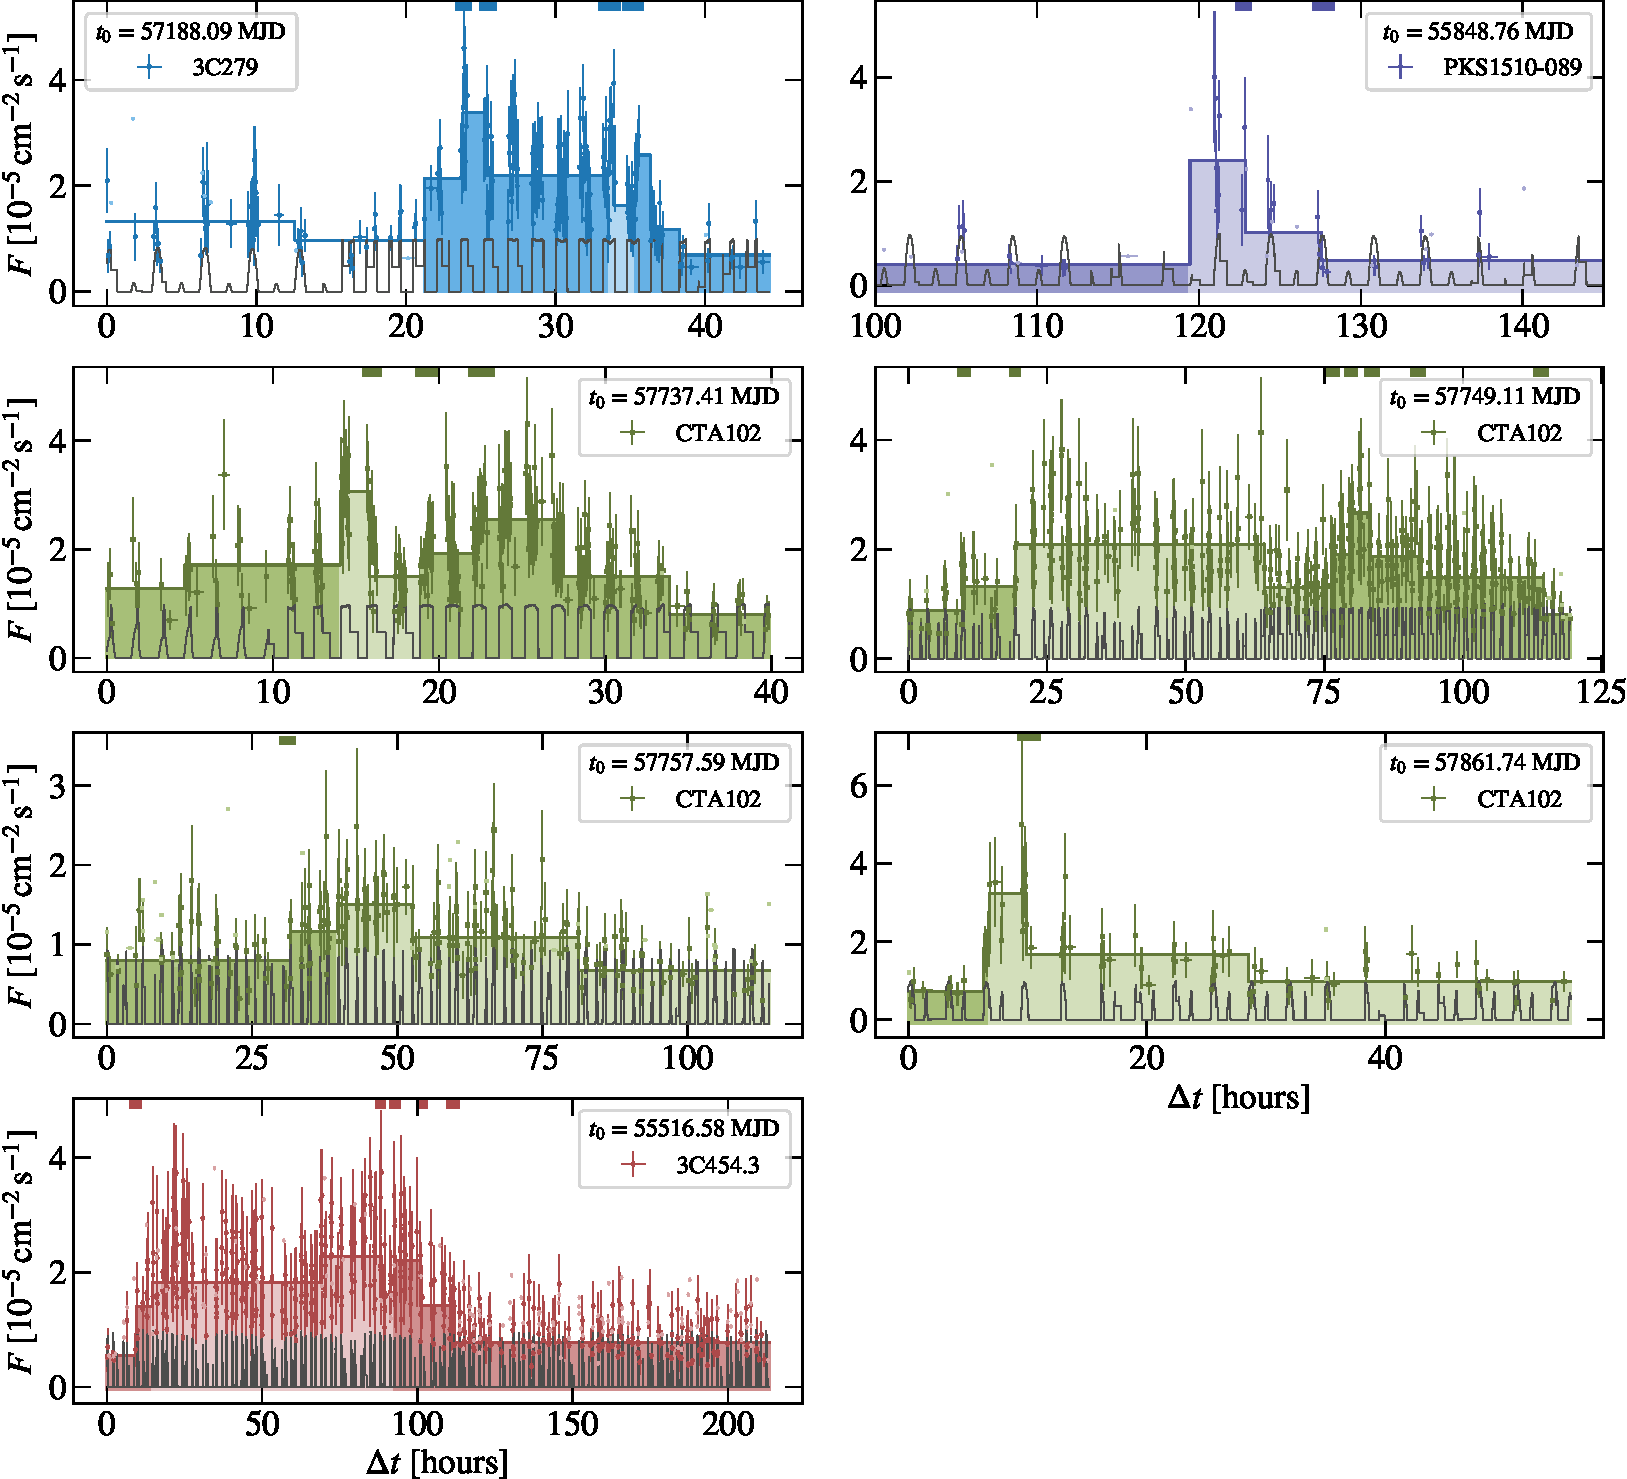
\includegraphics[width = .9\linewidth]{figures/lc_minute_3min.pdf}
    \caption{Sub-GTI light curves for the HOP groups of the orbital light curves which contain one bin with $\mathrm{TS} \geqslant 150$. The green shaded regions indicate GTIs that encompass a significant flux change found by the BB algorithm. The dark grey curves show the relative exposure at 1\,GeV \todo{check}. The ToO campaigns for 3C279 (upper left panel) and CTA102 (upper right panel) are clearly visible as the exposure is constant over several GTIs. }
    \label{fig:lc_minutes}
\end{figure*}

\begin{deluxetable}{cccccc}
\tablewidth{0pt}
\tabletypesize{\scriptsize}
\tablecaption{ \label{tab:minute}Results from sub-GTI light curves on minutes-scale variability.}
\tablehead{$t_0$ & $\Delta t$  & $\chi^2 / \mathrm{d.o.f.}$ & $p$-value & $p$-value& $\mathrm{min}(t_\mathrm{var})$  \\ 
{} [MJD] & [mins] & {} & {} & (post trial) & [mins]}
\startdata
\hline
\multicolumn{6}{c}{3C279}\\
\hline
57189.07 & 30.72 & 1.93 & 0.051 (1.95$\sigma$) & 0.188 (1.32$\sigma$) & $5.6\pm2.8$ \\
57189.14 & 35.13 & 1.68 & 0.071 (1.81$\sigma$) & 0.254 (1.14$\sigma$) & $3.6\pm1.4$ \\
57189.47 & 53.08 & 1.94 & 0.015 (2.42$\sigma$) & 0.060 (1.88$\sigma$) & $3.7\pm1.4$ \\
\hline
\multicolumn{6}{c}{PKS1510-089}\\
\hline
55854.07 & 50.80 & 2.01 & 0.091 (1.69$\sigma$) & 0.173 (1.36$\sigma$) & $7.9\pm5.0$ \\
\hline
\multicolumn{6}{c}{CTA102}\\
\hline
57738.07 & 37.04 & 2.30 & 0.011 (2.55$\sigma$) & 0.032 (2.14$\sigma$) & $2.8\pm1.0$ \\
57758.86 & 78.00 & 2.62 & 0.049 (1.97$\sigma$) & 0.049 (1.97$\sigma$) & $7.8\pm3.7$ \\
\hline
\multicolumn{6}{c}{3C454.3}\\
\hline
55520.25 & 25.83 & 1.96 & 0.048 (1.98$\sigma$) & 0.216 (1.24$\sigma$) & $3.2\pm1.6$ \\
\enddata
{
\tablecomments{The number of trials is counted for each flare individually and given by the number of green shaded areas in each panel of Fig.~\ref{fig:lc_minutes}.}
}
\end{deluxetable}


\section{Location of the $\gamma$-ray emitting region}
\label{sec:location}

The location of the \gray emission region in blazar jets remains unknown. 
From the rich data set of six FSRQs studied here, we attempt to constrain the position of the emitting region using two independent approaches. 
First, in Sec.~\ref{sec:blrabs}, we search for absorption signatures in the LAT spectra caused by pair production of \Grays with photons of external photon fields. We use spectra during the brightest flares identified in the orbital light curves in Fig.~\ref{fig:gti}.
The derived constraints are used to calculate energy dependent cooling times in Sec.~\ref{sec:tcool}, which will be compared against our results for the decay times for the whole energy range (see Sec.~\ref{sec:results-local}) and for energy dependent light curves.
As shown by~\citet{2012ApJ...758L..15D}, if the flux decay is dominated by radiative cooling in external radiation fields, the energy dependence of the decay times can be used to distinguish inverse-Compton cooling in the radiation fields of the BLR or the dust torus.
This provides additional information about the position of the \gray emission region.
Second, in Sec.~\ref{sec:gammaradio}, we search for time lags between \gray and radio emission. 
In the scenario where the non-thermal emission is triggered by, e.g., shocks propagating downstream through the jet, a time lag can be translated into the spatial separation between the radio and \gray emitting regions~\citep{2014MNRAS.445..428M}. 
With information about the location of the radio core, the position of the \gray emitting region can be constrained as well~\citep[e.g.,][]{2014MNRAS.441.1899F}. 

\subsection{Results from spectral fits to \gray data}
\label{sec:blrabs}
The attenuation due to pair production on a radiation field of soft photons should manifest itself as a cut-off feature in the \gray spectrum. 
The cut-off energy depends on the distance of the \gray emitting region to the central black hole, $r$, and the photon density of the considered photon field.
For FSRQs, photon densities of external radiation fields of the accretion disk, the BLR, and the extended dust torus usually dominate the one of internal synchrotron emission~\citep[see,e.g.,][]{2012ApJ...758L..15D}.
The most relevant external photon field for the \gray energies which can be probed with \FermiLAT is the BLR. 
Pair production on photons from the dust torus or the accretion disk only becomes important at energies beyond 1\,TeV, even when the \Grays are produced closed to the central black hole~\citep{finke2016}.

We therefore search for BLR absorption features by fitting the observed \gray spectra during the brightest flares with functions the form 
\begin{eqnarray}
    f(E,\vec{\pi},r,z) &=& f_\mathrm{int}(E,\vec{\pi}) \times \nonumber \\ &{}& \exp\left[-\left(\tau_{\gamma\gamma}^\mathrm{BLR}(E,r) +\tau_{\gamma\gamma}^\mathrm{EBL}(E,z) \right)  \right],
\end{eqnarray} 
where $f_\mathrm{int}(E, \vec{\pi})$ describes the intrinsic spectrum at \gray energy $E$ emitted by the source, which depends on spectral parameters, $\vec{\pi}$, and $\tau_{\gamma\gamma}^\mathrm{BLR / EBL}$ is the optical depth due to interactions of \Grays with BLR and EBL photons, respectively. 
For the EBL optical depth, which depends on $E$ and the source redshift, $z$, we use the EBL model of \citet{2011MNRAS.410.2556D}.
The BLR optical depth will depend on the \gray energy, the location of the \gray emission zone, and the BLR geometry. 
Here, we follow the stratified BLR model introduced by \citet{finke2016}, who models the BLR either as a collection of shells or rings perpendicular to the jet axis, in order to emulate a flattened BLR. 
Each shell or ring is assumed to have infinitesimal thickness and to emit a monochromatic UV or optical emission line. 
The radii $R_\mathrm{li}$ of the shells and rings as well as the line luminosities $L_\mathrm{li} = \xi_\mathrm{li}L_\mathrm{disk}$ are taken from templates of average spectra obtained in reverberation mapping campaigns relative to the radius and luminosity of the H$\beta$ line~\citep[see][for further details]{finke2016}.
With the H$\beta$ luminosities listed in Tab.~\ref{tab:src-select}, we fix the absolute luminosities (or conversely $\xi_{\mathrm{H}\beta}$) and radii of all lines included in the model.  
Together with the masses of the super-massive black holes, we can then calculate $\tau_{\gamma\gamma}^\mathrm{BLR}$ for both geometries as a function of $r$ and observed \gray energy $E$.
In the BLR model, the absorption is dominated by pair production with Ly$\alpha$ photons at rest-frame energy of $\epsilon_{\mathrm{Ly}\alpha}\sim10.2\,$eV emitted at radii between $\sim 8\times10^{16}$ and $2\times10^{17}$\,cm. 
In the ring geometry, the corresponding energy density, which is assumed to be isotropic in the stationary frame of the galaxy, becomes~\citep{finke2016}
    \begin{equation}
        u_\mathrm{BLR} \approx u_{\mathrm{Ly}\alpha}= \frac{\xi_{\mathrm{Ly}\alpha}L_\mathrm{disk}}{4\pi c(R_{\mathrm{Ly}\alpha}^2 + r^2)},
        \label{eq:u-blr}
    \end{equation}
and takes values $\sim 5\times10^{-2}\,\mathrm{erg}\,\mathrm{cm}^{-3}$ regardless of the source for $r = R_{\mathrm{Ly}\alpha}$.
These numbers can be compared against typical values for the BLR radius, $R_\mathrm{BLR} \sim 10^{17}\,\mathrm{cm}\, (L_\mathrm{disk} / 10^{45} \mathrm{erg}\,\mathrm{s}^{-1})^{1/2}$ \citep[e.g.][]{2007ApJ...659..997K,2009ApJ...697..160B} and energy density $u_\mathrm{BLR} \sim 10^{-2}\,\mathrm{erg}\,\mathrm{cm}^{-3} $ (again in the stationary galaxy frame) assuming  $L_\mathrm{BLR} = \xi_\mathrm{BLR} L_\mathrm{disk}$ with $\xi_\mathrm{BLR}\sim 0.1$. 
The chosen BLR model gives values broadly consistent with typical values within a factor of a few.

Typically, FSRQ spectra show intrinsinc curvature, even below energies at which BLR absorption becomes important (see, e.g., the 3FGL). Therefore we chose a log-parabola for the intrinsic spectral function and also test a power law with super-exponential cut-off. 
In the fit, we only include energy bins above 1\,GeV, as we expect the BLR cut-off at energies $\gtrsim 10\,$GeV. In this way, we avoid that the best fit is determined mainly by the high photon statistics below 1\,GeV.
Additionally, we select narrow time intervals around the brightest flares (see Sec.~\ref{sec:zoom} and Fig.~\ref{fig:gti}).
This is a compromise between sufficient photon statistics to probe energies above 10\,GeV and avoiding the mixing of different activity states with potentially different spectral states. 
From Fig.~\ref{fig:specvar} we see that for the highest fluxes only marginal spectral variability is present, which should render our results robust against potential variations of the intrinsic spectra. 
Also, we only include flares which have energy bins detected with $\mathrm{TS} > 0$ where the absorption exceeds 80\,\% for the smallest BLR distance tested ($r = 10^{-2}R_{\mathrm{Ly}\alpha})$. 
We skip a flare if this is not the case since no strong limits on $r$ can be derived in this case.
This excludes all flaring periods from 3C273, for which we cannot obtain any limits from the \gray spectra.

We derive the best-fit values for the spectral parameters $\vec{\pi}$ and the distance $r$ with a likelihood maximization of the bin-by-bin likelihood curves using \textsc{Minuit} \citep{},\footnote{The bin-by-bin likelihoods are derived by fixing the spectral shape in each bin to a power law and mapping the likelihood as a function of the normalization. In the process, the spectral parameters of the neighbouring point sources and diffuse backgrounds are fixed to their broad band best-fit values.} which we extract with \textsc{fermipy} and that are shown as gray shaded bands in the panels of Fig.~\ref{fig:seds}. 
The flux points in the figure coincide with the maximum likelihood. 
Also shown are the best-fit spectra and BLR attenuation for different distances $r$ (colored curves). 
We only include energy bins and their likelihoods if the bin-by-bin fit converged and if the source is detected with $\mathrm{TS} > 0$.\footnote{We do not have to limit ourselves to bins with even larger $\mathrm{TS}$, since our bin-by-bin likelihood approach takes full Poisson statistics into account. \todo{formulate a bit clerarer.}}


\begin{figure*}
    \centering
    \begin{tabular}{ccc}
    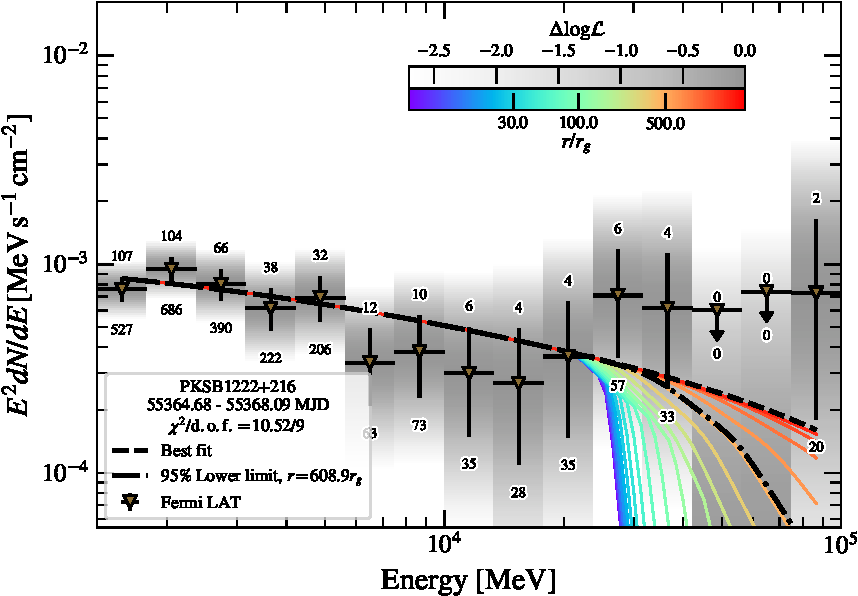
\includegraphics[width=0.32\linewidth]{figures/sed_PKSB1222+216_t001_LogParabola_3min_ring_emin1000.pdf} &
    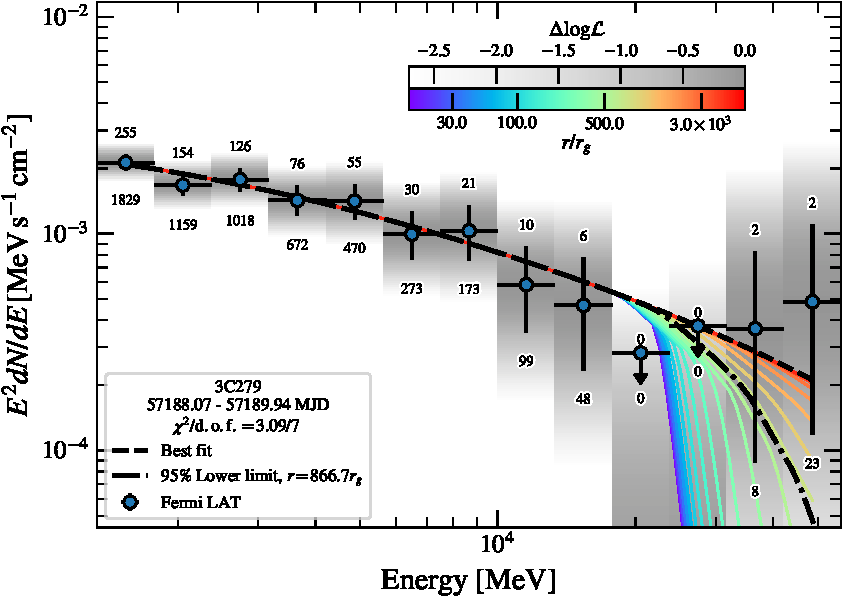
\includegraphics[width=0.32\linewidth]{figures/sed_3C279_t001_LogParabola_3min_ring_emin1000.pdf} & 
    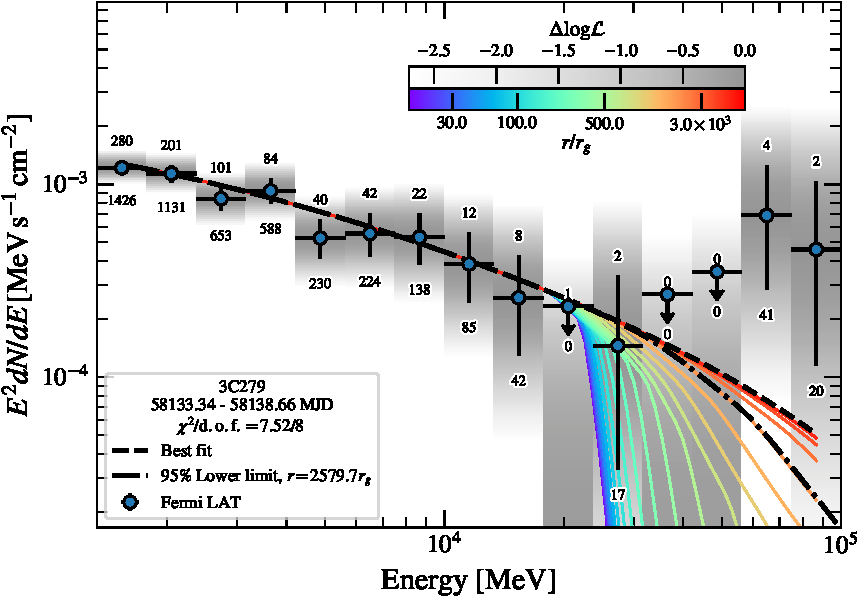
\includegraphics[width=0.32\linewidth]{figures/sed_3C279_t003_LogParabola_3min_ring_emin1000.pdf}\\
    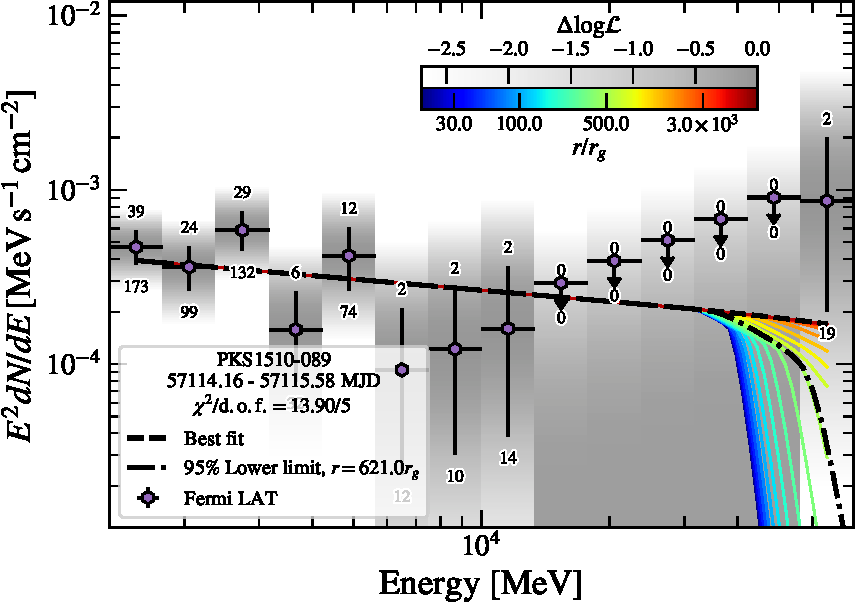
\includegraphics[width=0.32\linewidth]{figures/sed_PKS1510-089_t005_LogParabola_3min_ring_emin1000.pdf} &
    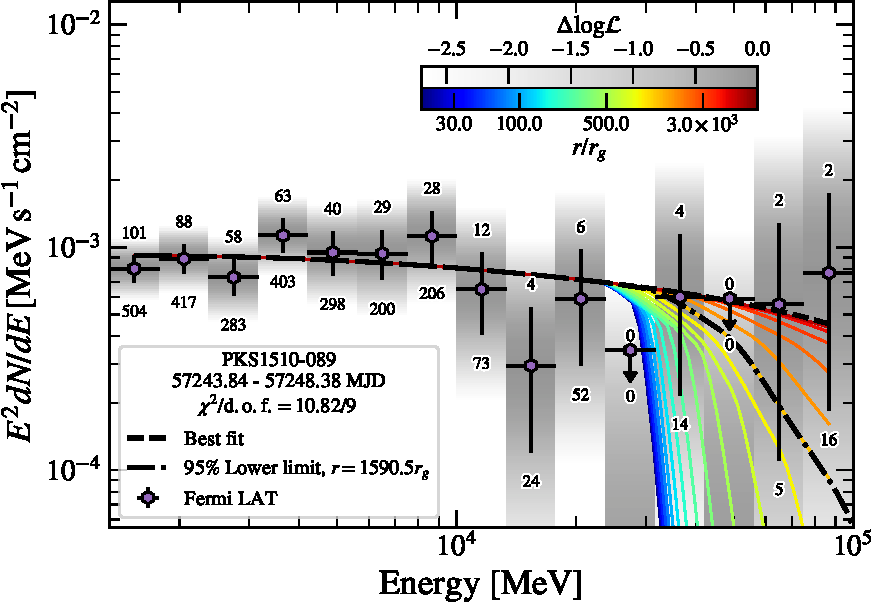
\includegraphics[width=0.32\linewidth]{figures/sed_PKS1510-089_t006_LogParabola_3min_ring_emin1000.pdf} & 
    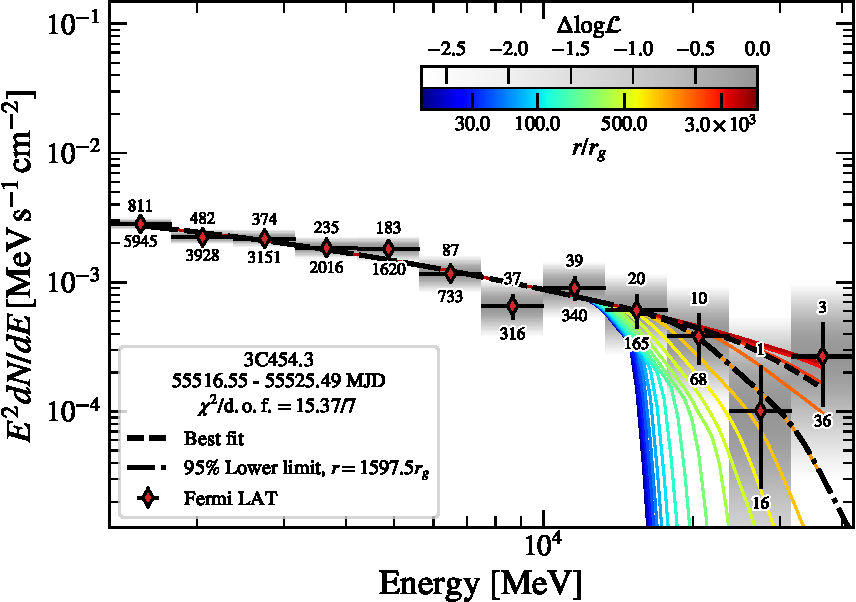
\includegraphics[width=0.32\linewidth]{figures/sed_3C454p3_t001_LogParabola_3min_ring_emin1000.pdf}\\
    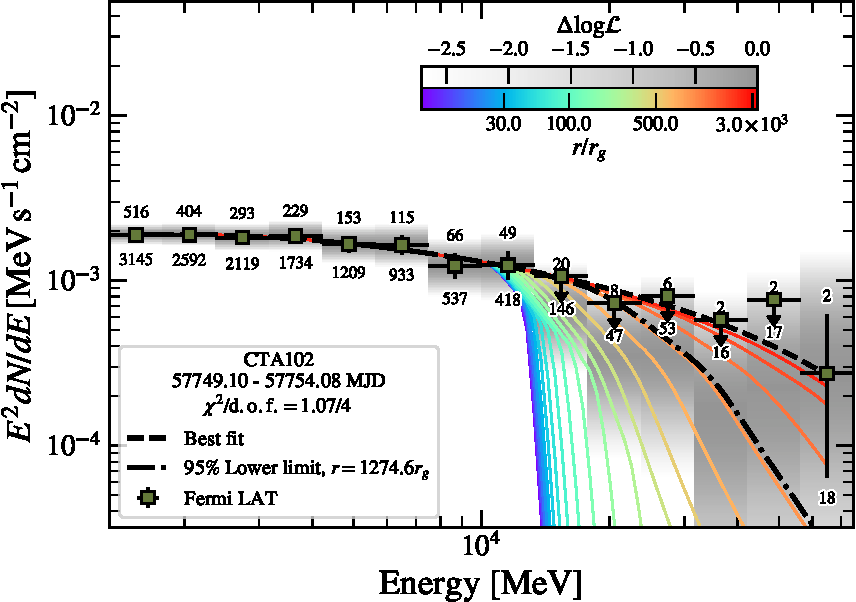
\includegraphics[width=0.32\linewidth]{figures/sed_CTA102_t002_LogParabola_3min_ring_emin1000.pdf} & 
    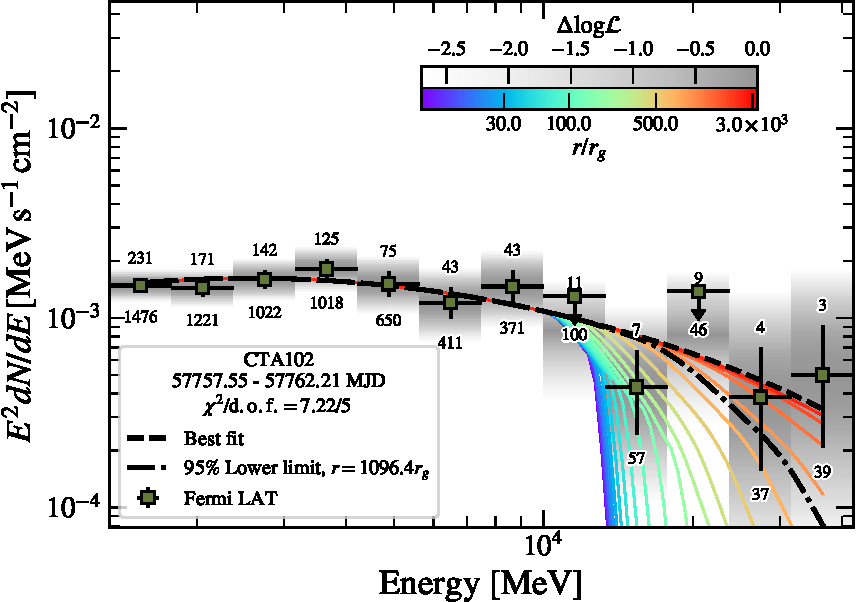
\includegraphics[width=0.32\linewidth]{figures/sed_CTA102_t003_LogParabola_3min_ring_emin1000.pdf} & 
    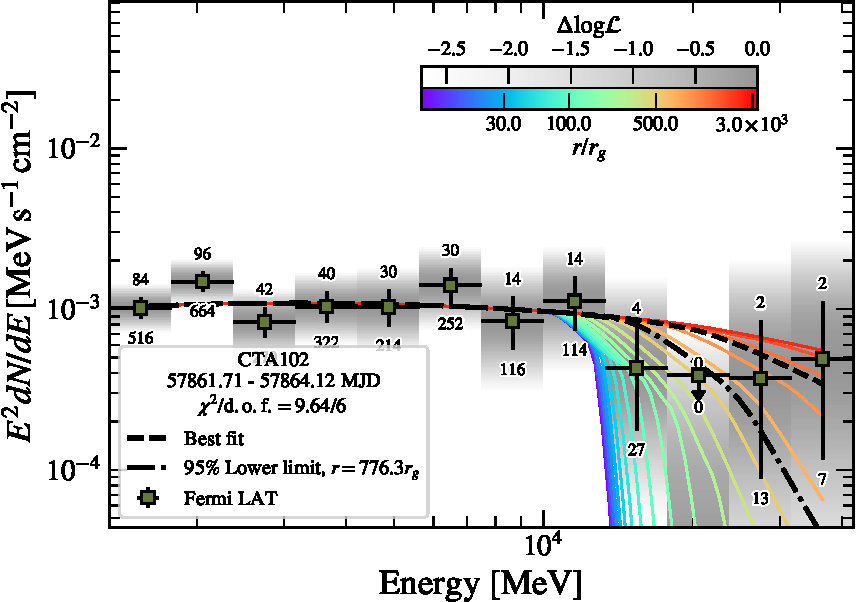
\includegraphics[width=0.32\linewidth]{figures/sed_CTA102_t004_LogParabola_3min_ring_emin1000.pdf}\\
    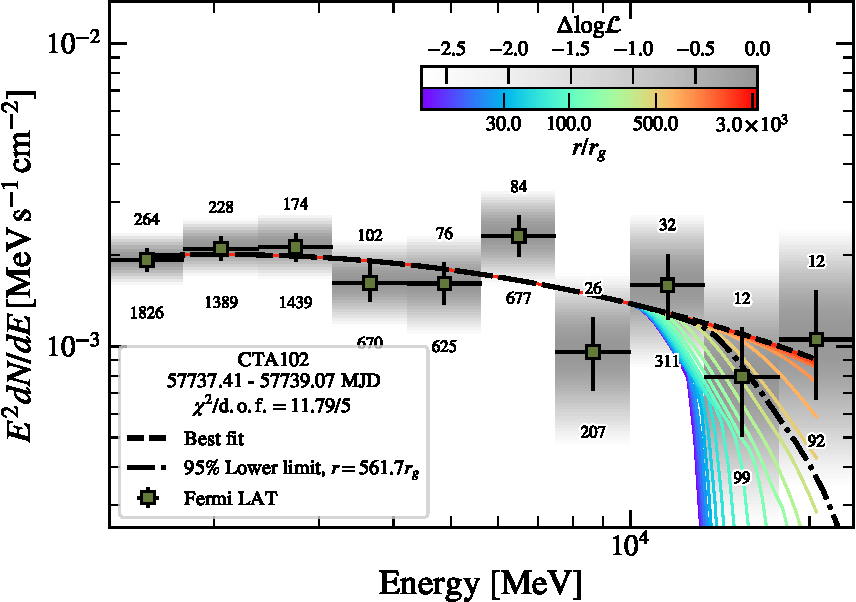
\includegraphics[width=0.32\linewidth]{figures/sed_CTA102_t001_LogParabola_3min_ring_emin1000.pdf}
    \end{tabular}

    \caption{Log-parabola fits above 1\,GeV to bright \gray flares detected at energies that correspond to a attenuation in the BLR of at least 20\,\% (for $r = 10^{-2}R_{\mathrm{Ly}\alpha}$). The attenuation due to the interactions with BLR photons (assuming the ring geometry) is shown as colored lines. The best fit (95\,\% lower limit on $r$) is shown as a black dashed (dash-dotted) line. 
    The fit uses the bin-by-bin likelihood curves shown as gray bands. The numbers below and above the flux points show the $\mathrm{TS}$ values  with which each bin is detected and the number of \Grays associated with the source at a probability $>85\,\%$, respectively.}
    \label{fig:seds}
\end{figure*}

For both tested BLR geometries, the best-fit value of $r$ is always close to or coincides with the maximum tested value, $r = 10R_{\mathrm{Ly}\alpha}$, and hence no significant absorption is found. found (dashed black lines in Fig.~\ref{fig:seds}). Consequently,  we use \textsc{Minos} to derive the profile likelihood as a function of $r$ from which we determine the 95\,\% lower limit on $r$ (dash-dotted black lines). 
The limit values are reported for each flare in Fig.~\ref{fig:blr_limits} and  summarized in Tab.~\ref{tab:blrabs} for the ring BLR geometry and log-parabola spectrum.
Assuming instead a power law with super-exponential cut-off yields consistent results. 
For the BLR shell geometry the lower limits are a factor of $\sim2$-$3$ higher because this geometry predicts stronger absorption~\citep{finke2016}. The ring geometry is therefore the conservative choice. 

As can be seen from Tab.~\ref{tab:blrabs} and Fig.~\ref{fig:blr_limits} the limits are of the order of $r_\mathrm{lim}\sim10^{17}$cm which translates to a distance close to or even beyond the Ly$\alpha$ emitting ring and consequently the BLR itself. In terms of gravitational radii, the emission regions should be located at distances of at least $\sim10^3r_g$. 
Table~\ref{tab:blrabs} also reports the energy of the highest energy photon (HEP) associated with the FSRQ with at least $99\,\%$ probability. For all but one source, this energy is larger than the energy where the optical depth due to absorption in the BLR exceeds $t_{\gamma\gamma}^\mathrm{BLR} > 1$ (assuming $r = r_\mathrm{lim}$). 

The limits depend sensitively on the detection of the source at energies as large as possible. To ensure that the detections are indeed not spuriuos, we also report the detection significance and the number of detected \Grays (associated with the source with a probability $>85\,\%$) for each energy bin below and above the flux points in Fig.~\ref{fig:seds}, respectively. The highest energy bins only contain a handful of source photons (1-4), which underlines the necessity to use the full Poisson likelihood information. 
Nevertheless, the source detections in these energy bins correspond to significances (approximated with  $\sqrt{\mathrm{TS}}$) $\gtrsim 4\,\sigma$.
The reason is that in the considered energies and short time spans (see Tab.~\ref{tab:blrabs}) the number of expected background events is small. 
\todo{comparison with costamante and others?}
\todo{comment on variability of BLR emission lines? See papers by Leon-Tavares 2013, 2015 and Isler 2015}
\todo{Isler 2015 find line emission variability on 3C454, PKS1510. There's also evidence for PKS1222. Brighter when also bright in \Grays. Might indicate IC scattering in BLR. However, also provides stronger absorption.} 
\todo{Leon Tavares 2013 also find brightening of line emission in 2010 flare of 3c454 consistent with the passage of superluminal jet component through radio core, could indicate that BLR clouds are also located at larger disntaces then assumed here. Easier to reconcile short variability times, but again, no absorption seen.}
\todo{Leon Tavares 2015: similar conclusion: BLR material might be located at distances $>$ 1pc. --- Also discuss absence of continuum radiation, ask Justin about it, check again Poutanen and Stern papers from 2010 and 2014}

\begin{figure}
    \centering
    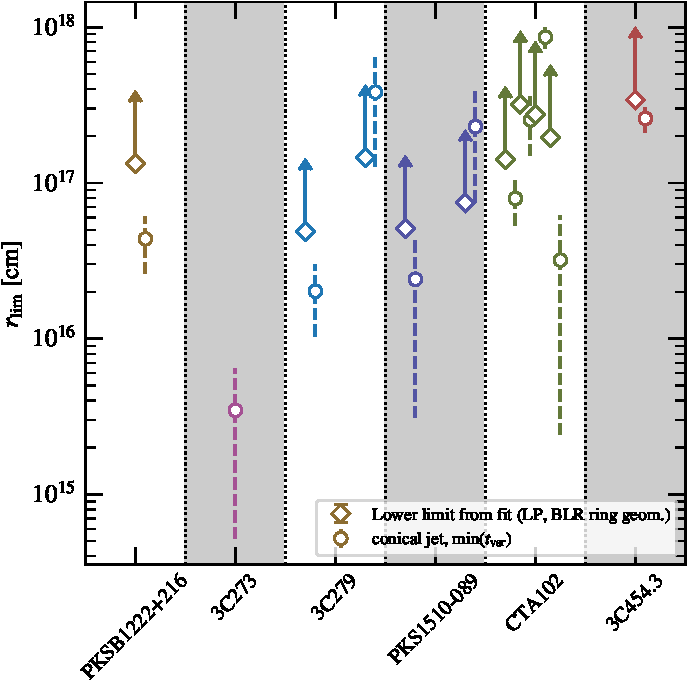
\includegraphics[width = .9\linewidth]{figures/limits.pdf}
    \caption{Lower limits on the distance $r$ of the \gray emitting region to the central black hole. Limits from fits to \gray spectra are shown as diamonds, values derived from variability considerations are shown as bullets. }
    \label{fig:blr_limits}
\end{figure}

\begin{deluxetable*}{ccccccc|ccc}
\tablewidth{0pt}
\tablecaption{ \label{tab:blrabs}Results from BLR absorption fits to \gray spectra.}
\tablehead{$t_0$ & $\Delta t$  & $r_\mathrm{limit}$ & 
$r_\mathrm{limit}$ & $r_\mathrm{limit}$  & $E_\mathrm{HEP}$  & $E_{\tau_{\gamma\gamma} = 1}$ & $t_\mathrm{cool,~BLR}$  &
$t_\mathrm{cool,~dt}$  & $\tau_\mathrm{decay}$\\
{} [MJD] & [days] & $[10^{17}\mathrm{cm}]$ & $[R_{\mathrm{Ly}\alpha}]$ & $[r_g]$ & [GeV] & [GeV] &  [mins] & [hours] & [hours]
}
\startdata
\hline
\multicolumn{10}{c}{PKSB1222+216}\\
\hline
55364.68 & 3.42 & 1.33 & 1.40 & 609 & 75.39 & 69.69 & 8.2 & 26.8 & $47.4\pm8.3$\\
\hline
\multicolumn{10}{c}{3C279}\\
\hline
57188.07 & 1.87 & 0.49 & 0.64 & 867 & 56.03 & 42.91 &  2.7 & 19.0 & $0.5\pm0.9$\\
58133.34 & 5.32 & 1.45 & 1.91 & 2580 & 92.56 & 107.91& 9.0 & 19.0 & $8.2\pm6.3$\\
\hline
\multicolumn{10}{c}{PKS1510-089}\\
\hline
57114.16 & 1.42 & 0.51 & 0.66 & 1088 & 66.54 & 54.99 & 0.6 & 4.5 & $0.4\pm0.3$\\
57243.84 & 4.53 & 0.74 & 0.97 & 1591 & 75.93 & 65.39 & 0.8 & 4.5 & $44.4\pm9.4$\\
\hline
\multicolumn{10}{c}{CTA102}\\
\hline
57737.41 & 1.67 & 1.41 & 0.86 & 562 & 36.25 & 21.23 & 1.0 & 6.4 & $0.3\pm0.5$\\
57749.10 & 4.99 & 3.20 & 1.95 & 1275 & 73.80 & 37.94& 2.8 & 6.4 & $8.7\pm1.2$ \\
57757.55 & 4.66 & 2.76 & 1.67 & 1096 & 39.19 & 32.38& 2.2 & 6.4 & $24.6\pm2.3$ \\
57861.71 & 2.42 & 1.95 & 1.18 & 776 & 34.73 & 24.94& 1.4 & 6.4 & $1.2\pm0.7$ \\
\hline
\multicolumn{10}{c}{3C454.3}\\
\hline
55516.55 & 8.93 & 3.19 & 1.36 & 1598 & 41.19 & 28.73& 4.2 & 16.8 & $2.6\pm1.0$ \\
\enddata
{
\tablecomments{Highest energy photons are given for source probabilities $> 0.99$. Decay time given for flare component with highest peak flux.}
}
\end{deluxetable*}

We also compare the limits from fits to \gray spectra to considerations from variability arguments in Fig.~\ref{fig:blr_limits}.
If the emission region $R'_\mathrm{blob}$ (the prime denotes the co-moving frame) is causally connected during the flare, the shortest variability time $t_\mathrm{var}$ set a lower limit on its size \citep[e.g.,][]{2008MNRAS.384L..19B}:
\begin{equation}
    R'_\mathrm{blob} \leqslant \frac{ct_\mathrm{var}\delta_\mathrm{D}}{1+z},  
\end{equation}
where $\delta_\mathrm{D} = \Gamma^{-1}(1 + \beta\cos\theta_\mathrm{obs})^{-1}$ is the Doppler boost factor with the bulk Lorentz factor of the flow, $\Gamma$, $\beta = \sqrt{1 - \Gamma^{-2}}$ the associated velocity, and $\theta_\mathrm{obs} $ is the angle between the line of sight and the jet axis.
Under the assumption of a conical jet with opening angle $\theta_\mathrm{j} \sim \Gamma^{-1}$, we obtain an upper limit on the distance to the black hole, $r \sim R'_\mathrm{blob}\Gamma \equiv r_\mathrm{j}$.
The values are plotted in Fig.~\ref{fig:blr_limits} for the minimum of the rise and decay times of the brightest flares found in Fig.~\ref{fig:gti}.
The average values for $\delta_\mathrm{D}$ and $\Gamma$ obtained from Very Long Baseline Array monitoring observations are used \citep{2017ApJ...846...98J}  and the total  uncertainty is obtained by summing the uncertainties on $\delta_\mathrm{D}$, $\Gamma$, and the fit uncertainty of $t_\mathrm{var}$ in quadrature.
In general, we find that $r_\mathrm{lim} \gtrsim r_\mathrm{j}$ indicating that the emission regions are at larger distances to the black hole than than predicted from the conical jet scenario.  

\subsection{Considerations from radiative cooling}
\label{sec:tcool}


With the limits on $r$ it is now possible to derive the energy density of the external photon field in the co-moving frame, which could be responsible for the \gray emission due to inverse-Compton (IC) scattering with relativistic electrons in the emission region. 
Because the cooling time depends on the energy density and in turn on $r$, a comparison between the predicted IC cooling times with the observed decay times could provide further information on where the \Grays are emitted.

In the galaxy frame, the energy density of the BLR in the ring geometry is approximately given by Eq.~\ref{eq:u-blr}, and hence the photon number density is $n_\mathrm{BLR} \approx u_\mathrm{BLR} / \epsilon_{\mathrm{Ly}\alpha}$.
Assuming that the BLR photon field is isotropic and in the limit $\Gamma \gg 1$, the energy density in the co-moving frame becomes:
$u'_\mathrm{BLR} = (4/3)\Gamma^2 u_\mathrm{BLR}$~\citep{1994ApJS...90..945D,2002ApJ...575..667D}.
We calculate the energy loss of the electrons, $\dot{\gamma}_\mathrm{BLR}'$, due to IC scattering in the co-moving frame numerically, in order to incorporate Klein-Nishina   effects following \citet{1970RvMP...42..237B}.
The observed cooling time is then given by
\begin{equation}
    t_\mathrm{cool,BLR} = \frac{1 + z}{\delta_\mathrm{D}} \frac{\gamma'}{\dot{\gamma}'_\mathrm{BLR}}.
    \label{eq:tcool}
\end{equation}
In the Thomson regime, this becomes
\begin{equation}
    t_\mathrm{cool,BLR} = \frac{1+z}{\delta_\mathrm{D}}\frac{3m_ec^2}{4c\sigma_\mathrm{T}u_\mathrm{BLR}'\gamma_\mathrm{BLR}'},
    \label{eq:tcool-thomson}
\end{equation}
where $m_e$ is the electron mass and $\sigma_\mathrm{T}$ the Thomson cross section. 
In what follows, we approximate the electron Lorentz factor with~\citep[e.g.,][]{2009herb.book.....D,finke2016}
\begin{equation}
    \gamma'_\mathrm{BLR} = \frac{1}{ \delta_\mathrm{D}}\sqrt{\frac{E_\mathrm{obs,BLR}(1+z)}{2\epsilon_{\mathrm{Ly}\alpha}}},
    \label{eq:gammaprime}
\end{equation}
where $E_\mathrm{obs,BLR}$ is the observed \gray energy of IC scattered BLR photons. 
From Eq.~\ref{eq:tcool-thomson} and \ref{eq:u-blr} it becomes clear that the cooling time scales as $t_\mathrm{cool, BLR}\propto r^2 \Gamma^{-2}$, i.e., the cooling becomes less efficient for large distances. 
Furthermore, if the \gray emission is produced very far away from the BLR, the external photons will appear as a point source illuminating the emission region from behind, so that $u'_\mathrm{BLR} = (1/4)\Gamma^{-2} u_\mathrm{BLR}$,~\citep{1994ApJS...90..945D} leading to an additional decrease of the cooling time with $\Gamma^2$. 
We again use the average values for $\delta_\mathrm{D}\sim31$ and $\Gamma\sim22$ derived from VLBA observations~\citep{2017ApJ...846...98J}.
The BLR cooling time for one flare of CTA102 is shown for $r=r_\mathrm{lim}$ and $r = 1\,$pc as a function of $\gamma'$ and $E_\mathrm{obs,BLR}$ in Fig.~\ref{fig:tcool} (black solid and dash-dotted lines, respectively). 
Klein-Nishina effects become important for $\gamma'_\mathrm{BLR} \gtrsim 2\times10^3$ or $E_\mathrm{obs,BLR}\gtrsim1\,$GeV and a clear departure from the Thomson regime in which 
$\sqrt{\gamma_\mathrm{BLR}'}$ (dashed and dotted black lines) becomes visible.
The decay times derived from the fit of the two bright flares of CTA102 around MJD 57738 are shown is dark green squares (see the first green shaded region in the panel in the 4th row and 2nd column in Fig.~\ref{fig:gti}), where one decay time is shown as an upper limit due to its large uncertainty. 
If the decay is indeed caused by IC scattering with BLR photons, a distance of $r\sim1\,$pc still seems to be compatible with the observed decay times. 
Similar conclusions can be drawn for the other sources in question. 
We provide the cooling times at 300\,MeV and the shortest decay times in Tab.~\ref{tab:blrabs}.

Figure~\ref{fig:tcool} also shows the variability time $t_\mathrm{var}$ derived for the sub-orbital period in Sec.~\ref{sec:sub-gti}, which is, however, in the rising part of the flare (cf. Fig.~\ref{fig:lc_minutes}). If equally short decay times were observed, this would suggest a distance $r \sim r_\mathrm{lim}$. \todo{mention different blobs?}

\begin{figure}
    \centering
    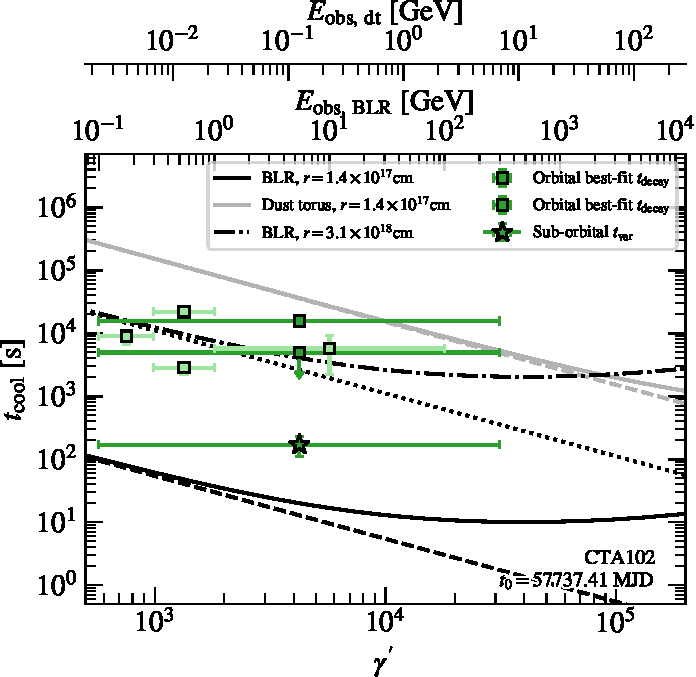
\includegraphics[width = .9\linewidth]{figures/tcool_CTA102_t001_LogParabola_ring.pdf}
    \caption{Cooling times for IC scattering with BLR photons and photons from the dust torus for one flaring episode of CTA102. Also shown are observed decay times for the full energy range, energy dependent light curves, and sub-orbital light curves.
    Note that the observed decay times are plotted with respect to IC scattering with BLR photons. For scattering with photons from the dust torus, the points need to be shifted to higher values of $\gamma'$ to match $E_\mathrm{obs,dt}$ (see second $x$-axis on the top of the figure).}
    \label{fig:tcool}
\end{figure}

  
As noted by \citet{2012ApJ...758L..15D}, the energy dependence of the cooling times could  further reveal the dominant photon field responsible for IC scattering: while Klein-Nishina effects become important already at 1\,GeV for scattering with BLR photons, the Thomson regime should be valid to higher energies for IC scattering with photons of the dusty torus (dt). 
Following again~\citet{finke2016}, we assume that the torus also has a ring geometry and emits monochromatic photons with energy $\epsilon_\mathrm{dt} = 2.7 k_B T_\mathrm{dt}$ with $k_B$ the Boltzmann constant and $T_\mathrm{dt} = 1000\,$K. 
The sublimation radius of the dust torus, $R_\mathrm{dt} = 3.5\times10^{18}\,\mathrm{cm}(L_\mathrm{disk}/10^{45}\,\mathrm{erg}\,\mathrm{s}^{-1})^{1/2}(T_\mathrm{dt}/10^3\,\mathrm{K})^{-2.6}$ is used for the ring radius. 
Making the appropriate substitutions in Eqs.~\ref{eq:u-blr}, \ref{eq:tcool}-\ref{eq:gammaprime}, we plot the cooling time $t_\mathrm{cool,dt}$ for $r = r_\mathrm{lim}$ as a grey line in Fig.~\ref{fig:tcool} (note the additional $x$-axis since $E_\mathrm{obs, BLR} \neq E_\mathrm{obs,dt}$). 
Indeed, Klein-Nishina effects only become relevant at $E_\mathrm{obs,dt} \gtrsim 10^2\,$GeV or $\gamma' \gtrsim 10^5$. The cooling times at $E_\mathrm{obs,dt} = 316\,$MeV are also provided in Tab.~\ref{tab:blrabs}.

To investigate this further, we split the energy range of our analysis into three energy bins, 
 from 100\,MeV-300\,MeV, 300\,MeV-1\,GeV, and 1\,GeV-100\,GeV and recompute the orbital light curves.
The energy bins are chosen as a compromise between number of bins and sufficient photon statistics in each bin. 
The light curves for which at least 2 BBs are identified in each energy bin are shown in Fig.~\ref{fig:lcebins}.
The decay times of fits to the energy dependent light curves are also plotted in Fig.~\ref{fig:tcool} (light green squares). Only for the 300\,MeV-1\,GeV the double peak of the flare is resolved and in general the fit qualities are rather poor with $\chi^2$ per degree of freedom between 1.67 and 2.26 for CTA102. This also explains the rather small error bars on $\tau_\mathrm{decay}$. 
From the fit values we cannot draw a conclusion whether the decay times evolve with $\sqrt{E_\mathrm{obs}}$ as expected in the Thomson regime.
Due to the lack of high photon statistics at energies beyond 10\,GeV where the differences become more pronounced, we are not able to use the method suggested by \citet{2012ApJ...758L..15D} to determine the photon field dominating the IC scattering. 
This conclusion also holds for the other tested sources. 

\begin{figure*}
    \centering
    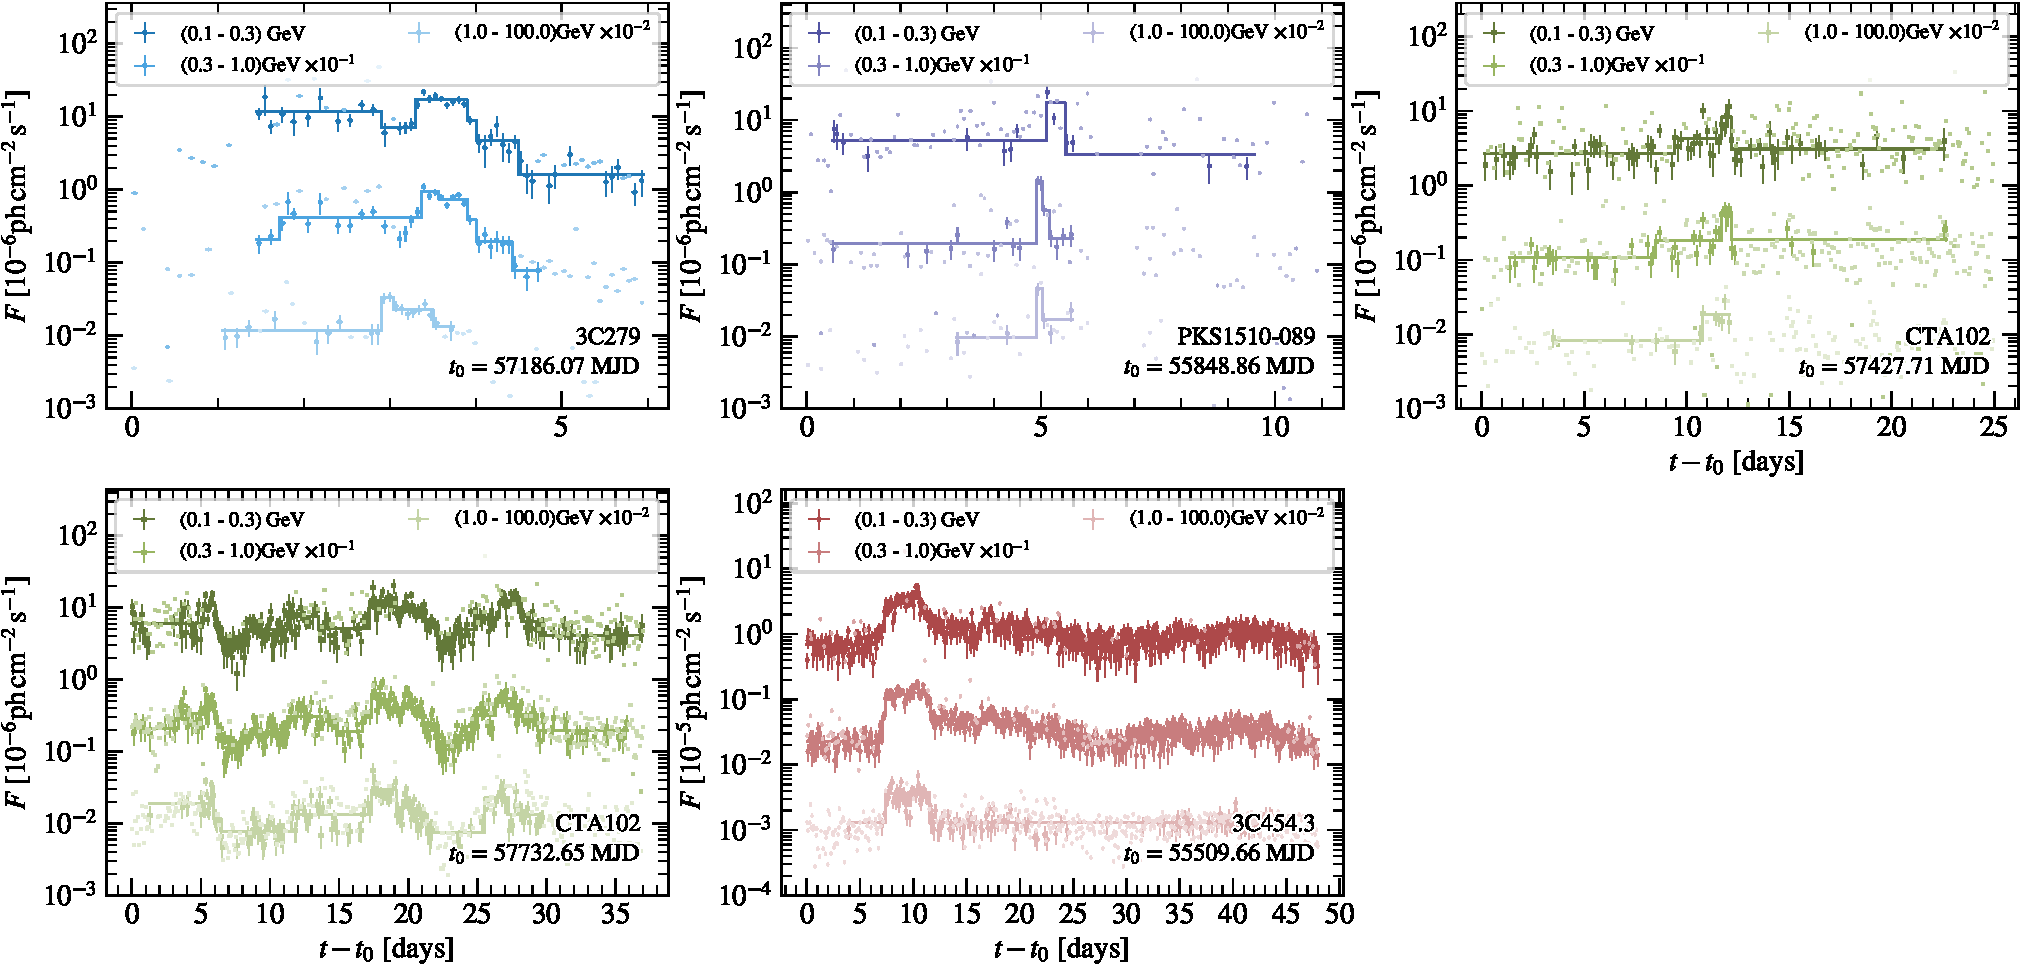
\includegraphics[width = .9 \linewidth]{figures/lc_ebins_ts9.pdf}
    \caption{\fermiLAT orbital light curves for three energy bins. The same time binning as in Fig.~\ref{fig:gti} is used. The thick colored lines indicate the BB representation. Only light curves are shown for which at least two BBs are identified for each energy bin.}
    \label{fig:lcebins}
\end{figure*}

Interestingly, the BBs for the energy dependent light curves of the flares for 3C279, PKS1510-089, and the last flare of CTA102 seem to indicate time lags between the energy bands, with the high-energy emission leading the low-energy \Grays.
For the 3C279 flare around MJD 57188, \citet{2015ApJ...808L..48P} could not find any time lags between the energy bins 0.1-1\,GeV and above 1\,GeV using the $Z$-transformed discrete correlation function \citep[DCF;][]{1997ASSL..218..163A,2013arXiv1302.1508A}.
Using the same methodology, we show the DCFs and their uncertainty for our energy dependent light curves with at least 2 BBs per energy bin in Fig.~\ref{fig:zdcf}.
We mark the time lags with horizontal lines at the maximum DCF values if $\mathrm{max}(\mathrm{DCF}) > 2 \sqrt{\mathrm{Var}(\mathrm{DCF})}$.
In contrast to \citet{2015ApJ...808L..48P}, we find evidence that the emission above 1\,GeV leads the emission at lower energies with $\sim 0.1$ days, howerver, from the fits to the light curves, the decay time at higher energies might actually be longer ($0.45\pm0.16$ days above 1\,GeV versus $0.22 \pm 0.03$ between 0.1 and 0.3\,GeV). 
Therefore, the lag might not be associated with cooling but rather with a changing particle injection. From the spectral variation (Fig.~\ref{fig:specvar}) it seems that the time bin before the peak of the flare might have a harder spectrum, however, the uncertainties are too large to draw firm conclusions.
For the CTA102 flare around MJD 57758 we also find that the high energy emission is leading, whereas for the flare at MJD 57749 the picture is reversed. 
For 3C454.3 the DCF also indicates that the low-energy emission is leading the high-energy emission, again suggesting that these lags are connected to the injection of particles rather than radiative cooling.

\begin{figure*}
    \centering
    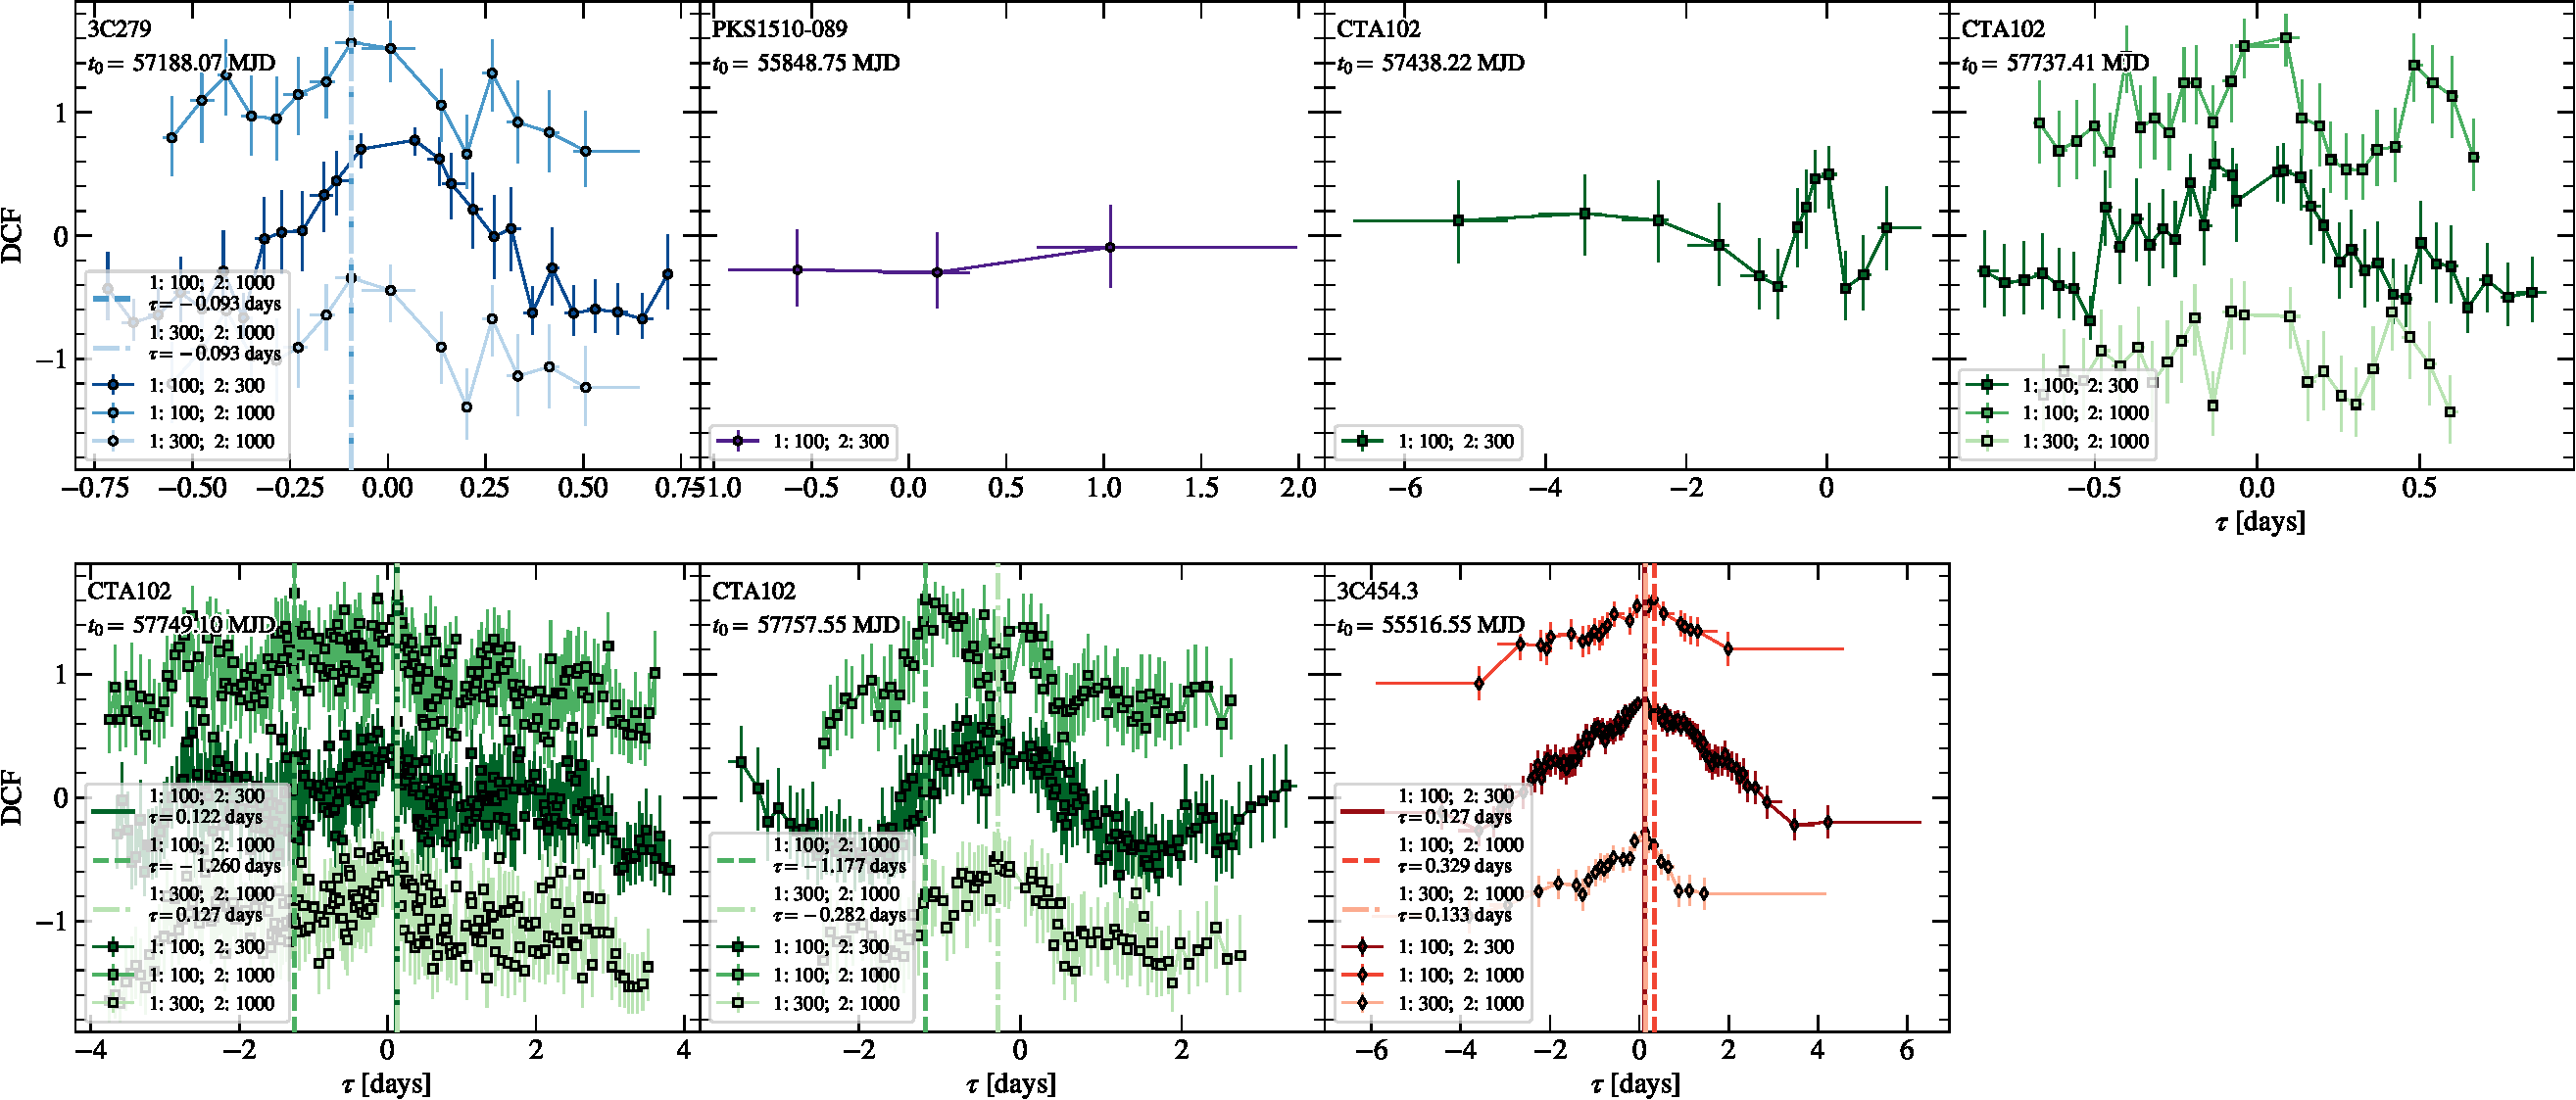
\includegraphics[width = .9 \linewidth]{figures/zdcf_ebins.pdf}
    \caption{Results for the DCF analysis for the light curves in Fig.~\ref{fig:lcebins}. In order to detect time lags for signle flares, the three flares of CTA102 starting at MJD 57733 are separated using the HOP groups. For time lags $\tau < 0$ the high-energy light curve leads the low-energy one. The DCFs between the energy bins starting at 0.1 and 1\,GeV and 0.3 and 1\,GeV are shifted by $\pm 1$ for better visibility. 
    Horizontal lines mark the maximum of the DCFs if $\mathrm{max}(\mathrm{DCF}) > 2 \sqrt{\mathrm{Var}(\mathrm{DCF})}$.}
    \label{fig:zdcf}
\end{figure*}



\subsection{Results from radio-\gray correlation analysis}
\label{sec:gammaradio}

Cross-correlating \gray light curves with radio light curves provides an alternative method to locate the \gray emitting region~\citep[e.g.,][]{2014MNRAS.441.1899F}.
Under the assumption that the flare is produced in a common emission confined region moving down the jet~\citep[e.g.,][]{2014MNRAS.445..428M},
the distance between the 
the \gray sphere, where the \gray opacity due to , e.g., absorption in the BLR, becomes less than unity~\citep{1995ApJ...441...79B}, and the 
radio core, where synchrotron-self-absorption becomes negligible~\citep[][]{1981ApJ...243..700K}, 
can be estimated from the time lag of the light curves.
The time lag, associated with a peak in the cross-correlation function between the \gray light curve and radio light curve obtained at frequency $\nu$, $\tau_{\mathrm{peak},r\nu}$, can be connected to the distance between the emission sites:
\begin{equation}
    d_{\gamma,r\nu} = \frac{\Gamma\delta_\mathrm{D}\beta c\tau_{\mathrm{peak},\gamma,r\nu}}{1 + z}.
    \label{eq:dgamma-r}
\end{equation}
Under the assumption that the radio emission lags the \Grays~\citep{}, the distance of the \gray emission region to the central black hole is thus $d_\gamma = d_{\mathrm{core},r\nu} - d_{\gamma,r\nu}$, where $d_{\mathrm{core},r\nu}$ is the position of the radio core at frequency $\nu$.
The core position itself is frequency dependent~\citep[the core shift effect, see, e.g.,][]{1998A&A...330...79L},
\begin{equation}
    d_{\mathrm{core},r\nu} = \frac{\Omega_{r\nu}}{\nu^{1/k_r}\sin\theta_\mathrm{obs}},
     \label{eq:core-shift1}
\end{equation}
where $k_r$ depends on the electron energy spectrum and the magnetic field in the emitting region~\citep{1981ApJ...243..700K} and
\begin{equation}
    \Omega_{r\nu} = 4.85\times10^{-9} \frac{\Delta r_\mathrm{mas} d_\mathrm{L}}{1 + z}\frac{\nu^{1/k_r}\nu_0^{1/k_r}}{\nu_0^{1/k_r}-\nu^{1/k_r}},
    \label{eq:core-shift2}
\end{equation}
where $d_\mathrm{L}$ is the luminosity distance and $\Delta r_\mathrm{mas}$ is the offset between the radio cores in milliarcseconds between the $\nu$ and a reference frequency $\nu_0$. 
The latter is related to the time lag between two radio light curves $\tau_{\mathrm{peak},r\nu_1,r\nu_2}$ through 
$\Delta r_\mathrm{mas} = \mu \tau_{\mathrm{peak},r\nu_1r\nu_2}$, where $\mu$ is the jet proper motion. 
The proper motion along with the core position at 15\,GHz has been measured by the 
MOJAVE blazar monitoring program along using very large baseline interferometry (VLBI) \citep{2012A&A...545A.113P,2016AJ....152...12L}.
The following distances $d_\mathrm{core,~15GHz}$ were determined  under the assumption that $k_r = 1$: for PKSB1222+216 $d_\mathrm{core,~15GHz}= 23.41\,$pc; for 3C279: $d_\mathrm{core,~15GHz}<7.88$\,pc; for PKS1510-089 $d_\mathrm{core,~15GHz} = 17.71\,$pc; for 
CTA102 $d_\mathrm{core,~15GHz} =46.7\,$pc; and for 3C454.3 $d_\mathrm{core,~15GHz} = 20.36\,$pc.
Dedicated analyses have also been carried out and found for 3C454.3 $k_r = 0.6$-$0.8$ and $d_\mathrm{core,~15GHz} \sim 38\,$pc and, since $d_{\mathrm{core},\nu}\propto\nu^{-1/k_r}$,  $d_\mathrm{core,~43GHz} \sim 9\,$pc~\citep{2014MNRAS.437.3396K}. 
For 3C273 \citet{2013ARep...57...34V} find $k_r = 1.4$ and $d_{\mathrm{core},\nu} = 134\nu^{-1/1.4}$ using radio observations at frequencies between 4.8 and 362 GHz.
Lastly, \citet{2015A&A...576A..43F} conducted VLBA observations of CTA102 ranging from 5\,GHz to 86\,GHz and found $k_r = 1.0$ as a best-fit value and $d_{\mathrm{core,~86GHz}}\sim7\,$pc.
Provided that we can estimate $\tau_{\mathrm{peak,15GHz}r\nu}$, it is possible with the above results to estimate the core position at arbitrary radio frequency $\nu$ using Eqs.~\ref{eq:core-shift1} and \ref{eq:core-shift2}.
In order to arrive at an estimate for $d_\gamma$ the only remaining task is to perform a cross correlation study between \gray and radio light curves.
\todo{this sentence might need some update, describe methods and results first}

We search for time lags between the \fermiLAT light curves and radio light curves obtained with the Owens Valley Radio Observatory (OVRO) at 15\,GHz, the Atacama Large submillimeter/millimeter Array (ALMA) between 84 and 116\,GHz (Band 3, 3.6\,mm-2.6\,mm), and the Submillimeter Array (SMA) at 230\,GHz (1.3\,mm). 
All of the studied FSRQs are included in an ongoing blazar monitoring program at OVRO~\citep{2011ApJS..194...29R} and SMA~\citep{2007ASPC..375..234G}, and also serve as calibrators for SMA and ALMA~\citep{2018MNRAS.478.1512B} at mm wavelengths.\footnote{Data from the observatories are available at \url{http://www.astro.caltech.edu/ovroblazars}, \url{https://almascience.eso.org/alma-data/calibrator-catalogue}, and \url{http://sma1.sma.hawaii.edu/callist/callist.html}.}
We show all radio and \gray light curves in Fig.~\ref{fig:lc-radio}.
It is evident that the OVRO light curves show variations and longer time scales and less flicker noise behavior and at least for 3C454.3 their appears to be a correlation between the radio and \gray flux at least for the giant flare in 2010 (around MJD\,55500). 
Due to scarce and uneven sampling, we do not use the ALMA and SMA light curves of PKSB1222+216 and PKS1510-089.
We further do not include the SMA light curve of CTA102 in the following analysis for the same reason.

\begin{figure*}
    \centering
    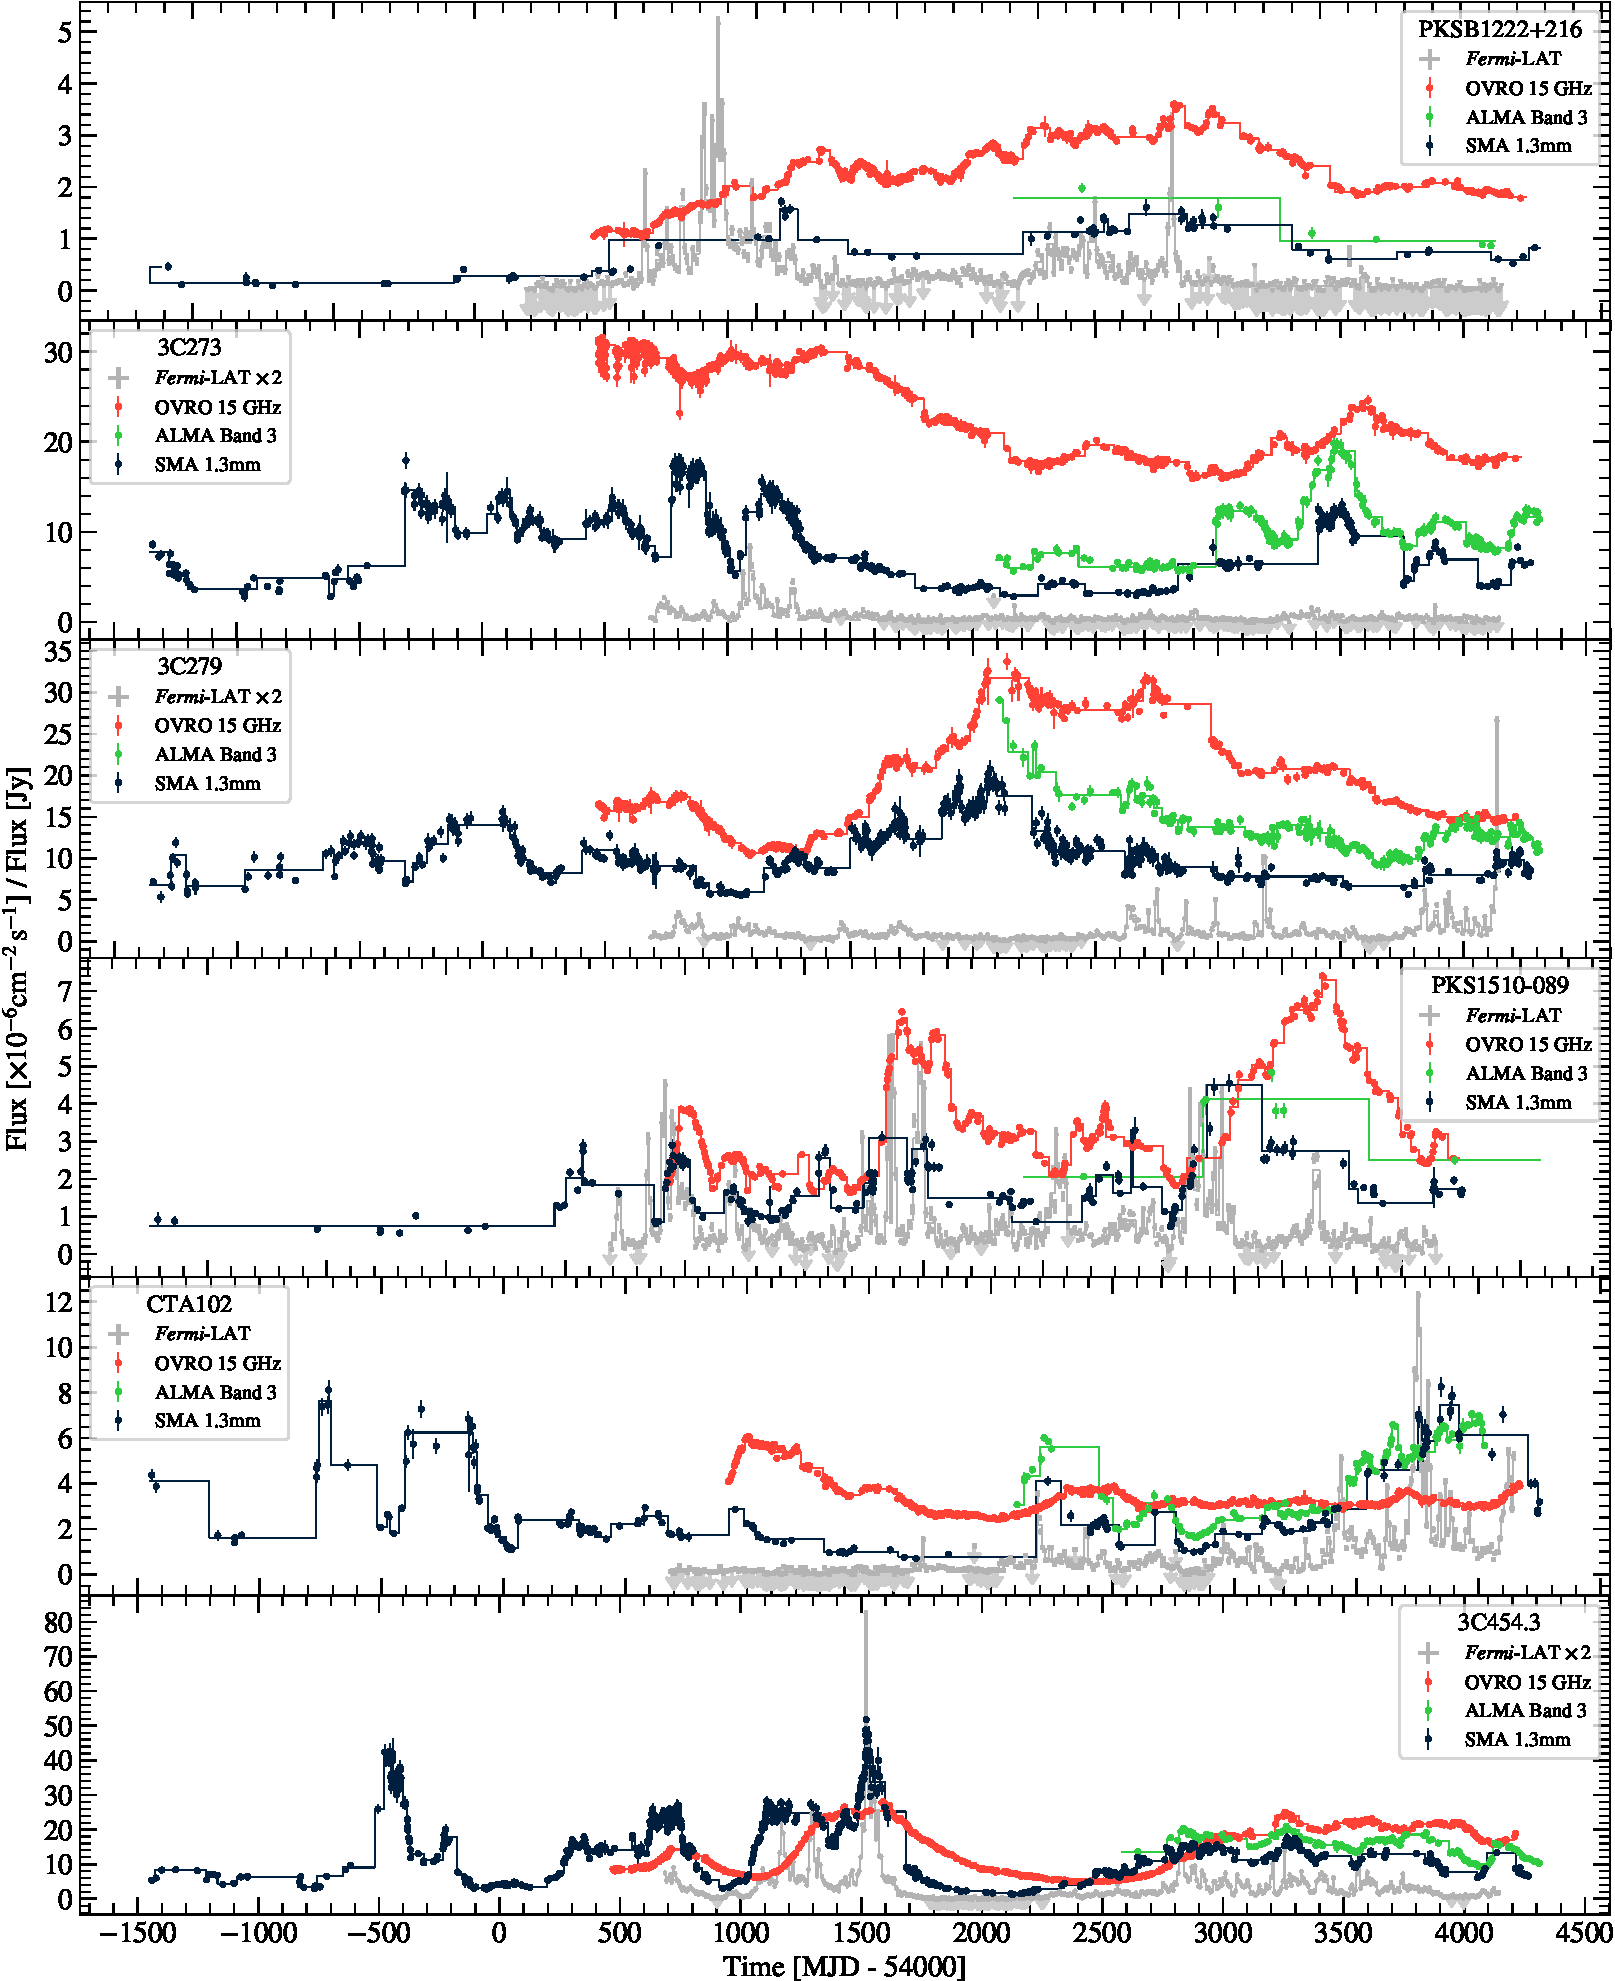
\includegraphics[width = .9\linewidth]{figures/lc_gamma_radio_tsmin9.pdf}
    \caption{Radio and \gray light curves normalized to the maximum flux.}
    \label{fig:lc-radio}
\end{figure*}

To quantify these observations, we again closely follow the methodology laid out by \citet{2014MNRAS.445..437M}. 
For two light curves with fluxes $a_i$ and $b_j$ with uncertainties $\sigma_{ai}$ and $\sigma_{bj}$ measured at times $t_{ai}$ and $t_{bj}$ we compute the local cross correlation function
\begin{equation}
\mathrm{LCCF}(\tau) = \frac{1}{M}\frac{\sum(a_i - \bar{a}_\tau)(b_j - \bar{b}_\tau)}{\sigma_{a\tau}\sigma_{b\tau}},
\end{equation}
where the sum runs over the $M$ pairs for which $\tau \leqslant t_{ai} - t_{bj} < \tau + \Delta t$, for some chosen time step $\Delta t$, and $\bar{a}_\tau$ and $\bar{b}_\tau$ and $\sigma_{a\tau}$ and $\sigma_{b\tau}$ are the flux averages and standard deviations over the $M$ pairs, respectively~\citep{1999PASP..111.1347W}. 
The LCCF is bounded between $-1$ and $1$ and has much larger efficiency in recovering linear correlations between light curves compared to the discrete correlation function \citep{2014MNRAS.445..437M}.
We also prefer this method over the $Z$-tranformed DCF used in Sec.~\ref{sec:tcool} because it is possible to assign a significance to a time lag corresponding to the maximum value of the LCCF using simulated light curves as outlined below. 
For the binning of the time lags $\tau$ we choose the half the maximum of median of the time separations between consecutive data points in each light curve.
The minimum and maximum values of $\tau$ is chosen to be $\pm0.5$ times the length of the shortest light curve~\citep{2014MNRAS.445..428M}.

We determine the significance of a peak in the LCCF by cross correlating pairs of simulated light curves. 
For the \gray light curves, the simulation proceeds in the same way as described in Sec.~\ref{sec:results-global}, where we use the best-fit values $\hat{\beta}$ for the assumed PSD.
For the radio light curves, we proceed in a similar way. 
First, we determine the best-fit PSD similar to the \gray light curves. 
In order to achieve a good fit between the observed and simulated PSDs we change the methodology used for the \gray light curves in the following ways:
instead of matching the flux PDFs of the light curves as suggested by \citet{2013MNRAS.433..907E}, we use variance matching~\citep{2014MNRAS.445..437M}. For radio light curves, the best-fit slopes are much closer to $\beta \sim 2$, so that Parseval's theorem applies.
Furthermore, we do not apply uncertainties to the simulated light curves. 
Doing so generally leads to a strong flattening of the periodograms at high frequencies when they become dominated by white noise introduced by the uncertainties. 
This is not observed in the periodogram derived from the observations. 
The reason for this might be a correlation between uncertainties and flux, which is not taken into account by the adopted simulation scheme, leading to an overestimation of the simulated uncertainties.
Lastly, the radio light are unevenly sampled and can show large observational gaps. 
Simply applying the interpolation scheme used for the the \gray light curves would mean that most data points that enter the calculation of the periodogram are actually interpolated data points. 
To mitigate this problem, we split the light curves where they show large gaps. 
We found that a split at gaps that are 20 (4.5) times larger than the median separation between consecutive measurements for OVRO and SMA (ALMA) light curves provides a good compromise between minimizing the number of splits and too few data points within a light curve segment. 
Furthermore, for the interpolated light curves we use a time step equal the 80\,\% quantile of the observed separation (the median would correspond to the 50\% quantile). 
In this way, we loose sensitivity to the highest frequencies but end up with interpolated light curves with roughly the same number of data points as the observed one. 
We do not average the interpolated flux points as in the \gray case since radio observations are usually short in duration and report flux densities instead of integrated fluxes. 
The periodograms of the individual light curve segments are finally log averaged following \citet{1993MNRAS.261..612P}.

We report the best-fit slopes of the assumed power-law PSDs $\hat{beta}$, their confidence interval, and the $p_\beta$-value of the fit in Tab.~\ref{tab:lccf}.
The confidence interval and $p_\beta$-value are determined in the same way as described in Sec.~\ref{sec:results-global}.
For the SMA and OVRO light curves for 3C454.3, we are only able to provide upper bounds on $\beta$.
In general we confirm the trend that the OVRO light curves show a softer PSD $\hat{\beta} \gtrsim 2$ for all sources. 
Moving to higher frequencies with ALMA and SMA, the PSD hardens and becomes more flicker-noise like. 
We can compare our results for the OVRO light curves to previous analyses of \citet{2014MNRAS.445..428M} who used 4 years of data, and find them to generally consistent within uncertainties. 

Having determined the best-fit PSD, we use it to create artificial light curves in the same way as for fitting the periodogram using the best-fit PSD slope as an input.
We then calculate the LCCF between 5000 pairs of un-correlated simulated light curves to derive confidence bands on the LCCF and to determine the $p_\tau$-value, which gives the probability to find an LCCF value at given $\tau$ greater or equal to the observed value under the assumption that the light curves are un-correlated. 

\begin{deluxetable*}{l|cc|ccc}
\tablewidth{0pt}
\tablecaption{ \label{tab:lccf}Results from PSD analysis of radio light curves as well as \gray and radio LCCF results.}
\tablehead{Source & $\hat{\beta}$ & $p_\beta$ & $\tau_\mathrm{peak}$ [days] & $p_\tau$ & $d_{\gamma, r}$ [pc]}
\startdata
\hline
\multicolumn{6}{c}{OVRO}\\
\hline
PKSB1222+216 & $1.92^{+0.39}_{-0.59}$ & 0.59 & --- & --- & ---\\
3C273 & $2.38^{+0.30}_{-0.97}$ & 0.94 & $-416.5^{+217.0}_{-140.0}$ & 0.0068 & $10.96~[5.2,14.6]~\pm4.4$\\
3C279 & $2.29^{+0.32}_{-0.94}$ & 0.71 & --- & --- & ---\\
PKS1510-089 & $1.89^{+0.45}_{-0.84}$ & 0.34 & --- & --- & ---\\
CTA102 & $2.23^{+0.26}_{-0.92}$ & 0.84 & --- & --- & ---\\
3C454.3 & $2.20^{+0.36}_{-2.20}$ & 0.40 & $-101.5^{+49.0}_{-112.0}$ & 0.0156 & $15.39~[8.0,32.4]~\pm2.8$\\
\hline
\multicolumn{6}{c}{ALMA Band 3}\\
\hline
3C273 & $2.12^{+0.40}_{-2.12}$ & 0.73 & --- & --- & ---\\
3C279 & $1.82^{+0.38}_{-0.45}$ & 0.89 & --- & --- & ---\\
CTA102 & $1.94^{+0.42}_{-1.33}$ & 0.45 & $-216.0^{+209.0}_{-11.0}$ & 0.0092 & $58.85~[1.9,61.8]~\pm7.3$\\
3C454.3 & $1.73^{+0.36}_{-0.30}$ & 0.25 & $-27.0^{+30.0}_{-30.0}$ & 0.0164 & $4.09~[-0.5,8.6]~\pm0.7$\\
\hline
\multicolumn{6}{c}{SMA 1.3mm}\\
\hline
3C273 & $1.48^{+0.40}_{-0.33}$ & 0.17 & $-122.5^{+84.0}_{-7.0}$ & 0.0088 & $3.22~[1.0,3.4]~\pm1.3$\\
3C279 & $1.61^{+0.16}_{-0.28}$ & 0.97 & --- & --- & ---\\
3C454.3 & $1.64^{+0.31}_{-1.64}$ & 0.21 & $10.5^{+21.0}_{-28.0}$ & 0.0002 & $-1.59~[-4.8,2.7]~\pm0.3$\\
\enddata
{
\tablecomments{For the LCCF analysis we only report time lags $< 0 $ and with a significance $p_\tau < 0.05$. The range of $d_{\gamma r}$ reported in square brackets are due to the uncertainty on $\tau_\mathrm{peak}$, the remaining uncertainties are the propagated errors on $\Gamma$ and $\delta_\mathrm{D}$.}
}
\end{deluxetable*}

We show the LCCF between \gray and radio light curves in Fig.~\ref{fig:lccf} for the cases where we find a peak in the LCCF at a significance $p_\tau$-value $<0.05$. Time lags $\tau < 0$ mean that the \gray light curve leads the radio light curve. 
We estimate the uncertainty on the peak time using flux randomization and random subsample selection (drawing 1000 samples) following \citet{1998PASP..110..660P} as suggested by \citet{2014MNRAS.445..437M}.
The peak and the uncertainties are marked by a dotted line and shaded region. 
They are also summarized together with the $p_\tau$ values in Tab.~\ref{tab:lccf}.
We only consider peaks with $\tau < 0$, however, 
for 3C273 and 3C454.3 peaks with $\tau > 0$ are also visible. 
For 3C454.3 these peaks occur at large values of $\tau$ that might be due to the several small flares observed at \gray energies. Since the overlap between the light curves is smaller for larger values of $|\tau|$ we deem this peaks less credible. 
For 3C273 the situation is less clear. 
The SMA light curve shows two prominent flares around the 
\gray flare they give rise to the two peaks. 
The low state of the source in recent years and the less dense sampling of the SMA light curve render it difficult to draw firm conclusions. As we see below, even the peak at $\tau < 0$ does not lead to constraints on the position of the \gray emitting region. \todo{CHECK!}.

\begin{figure*}
    \centering
    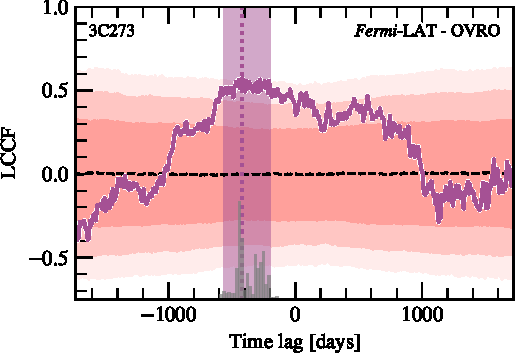
\includegraphics[width = .32\linewidth]{figures/lccf_3C273_nsim5000_fermi_EM13gaps-data_ovro_MM14gaps-none_lccf.pdf}
    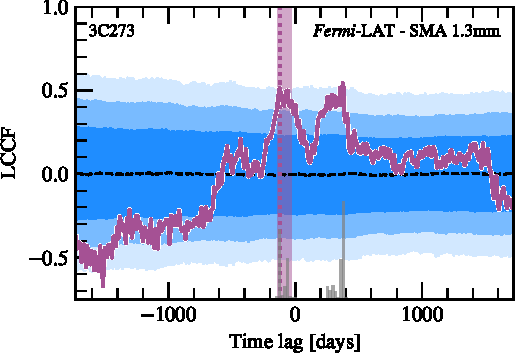
\includegraphics[width = .32\linewidth]{figures/lccf_3C273_nsim5000_fermi_EM13gaps-data_sma-1p3mm_MM14gaps-none_lccf.pdf}
    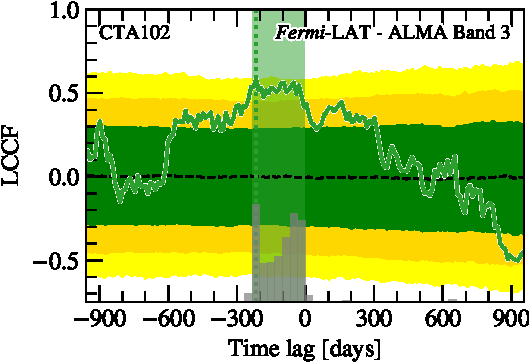
\includegraphics[width = .32\linewidth]{figures/lccf_CTA102_nsim5000_fermi_EM13gaps-data_alma-band3_MM14gaps-none_lccf.pdf}
    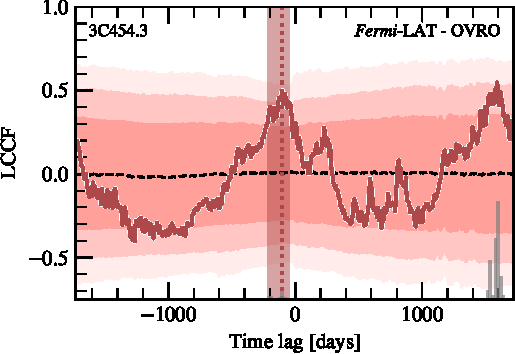
\includegraphics[width = .32\linewidth]{figures/lccf_3C454p3_nsim5000_fermi_EM13gaps-data_ovro_MM14gaps-none_lccf.pdf}
    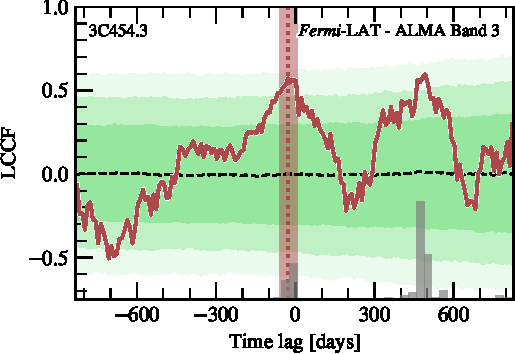
\includegraphics[width = .32\linewidth]{figures/lccf_3C454p3_nsim5000_fermi_EM13gaps-data_alma-band3_MM14gaps-none_lccf.pdf}
    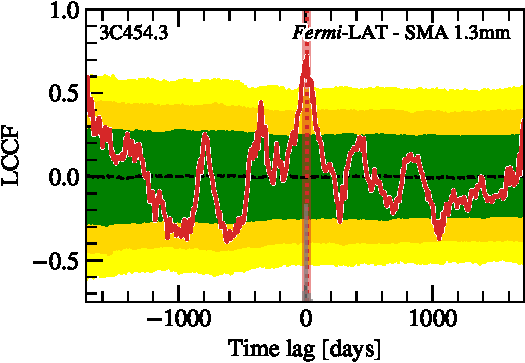
\includegraphics[width = .32\linewidth]{figures/lccf_3C454p3_nsim5000_fermi_EM13gaps-data_sma-1p3mm_MM14gaps-none_lccf.pdf}
    \caption{LCCF between \gray and radio light curves for the cases where a significant time lag, $p_\tau < 0.05$ is found. The vertical dotted line and shaded regions show the time lag peaks (for $\tau < 0$) and their uncertainty. 
    The green, dark yellow, and bright yellow colored regions denote the 68\,\%, 95\,\%, and 99\,\% envelopes derived from simulated un-correlated light curve pairs. 
    The grey histograms show the number of $\tau_\mathrm{peak}$ values obtained from flux randomization and random subsample selection to estimate the uncertainty on $\tau_\mathrm{peak}$.}
    \label{fig:lccf}
\end{figure*}

Using Eq.~\ref{eq:dgamma-r} and the peak identified in the LCCF, we can now derive the distance between the \gray and radio emitting region. 
The most significant lag is found for SMA and \gray light curves of 3C454.3 with $p_\tau = 2\times10^{-4}$ ($3.72\sigma$). 
Taking the uncertainties on $\tau_{\mathrm{peak},\gamma,230\mathrm{GHz}}$ into account, 
the time lag, and hence $d_{\gamma,r}$, is consistent with zero.
A similar conclusion is reached for the ALMA light curve even though it does not cover the major outbreak in 2010. 
For the correlation with the OVRO light curve, a longer time lag $\tau_{\mathrm{peak},\gamma,15\mathrm{GHz}} = -102$ days is found, placing $d_{\gamma,r}$ between $\sim 5$ and 35\,pc.
This time lag is consistent with the recent DCF analysis carried out by \citet{2018MNRAS.480.5517L} who found a time lag of $(115\pm6)$\,days at $2.5\,\sigma$ significance using 8\,years of OVRO data and the \fermiLAT weekly monitored light curve. 

For CTA102, we only find a significant LCCF between the ALMA and \gray light curve. 
The time lag translates into $d_{\gamma,r} \sim [-5;69]\,$pc taking uncertainties on $\tau_{\mathrm{peak},\gamma,100\mathrm{GHz}}$ as well as $\Gamma$ and $\delta_\mathrm{D}$ into account.
Hence, the distance is also consistent with zero. 

We find significant correlation between the \gray light curve of 3C273 and both light curves of SMA and OVRO. 
For the 15\,GHz OVRO light curve $d_{\gamma,r}$ is found between 0.8 and 19\,pc whereas for 230\,GHz the distance falls between $-0.7$ and 4.7\,pc and is consistent with zero. 

Lastly, we determine the position for the $\sim100$\,GHz (ALMA) and $230\,$GHz core (SMA) using a cross-correlation between the radio light curves to derive $\tau_{\mathrm{peak},15\mathrm{GHz},r\nu}$.
Using Eqs.~\ref{eq:core-shift1} and \ref{eq:core-shift2} we arrive at the new core position, where we use the average values of the measured jet proper motion~\citep[see Table 4 in][]{2016AJ....152...12L}, the observation angle $\theta_\mathrm{obs}$ reported in \citet{2017ApJ...846...98J},
and values $k_r$ found in the dedicated analyses discussed above. 
The results and their uncertainties are summarized in Tab.~\ref{tab:lccf-radio}.
For 3C273 and 3C454.3 we find that our core positions are consistent with values calculated from the $d_\mathrm{core}\propto\nu^{-1/k_r}$ relation obtained by \citet{2013ARep...57...34V} and \citet{2014MNRAS.437.3396K}, respctively. 
This is a non-trivial results since we have combined our time lags with jet proper motions from MOJAVE and jet properties from VLBA observations. 

Combining the core positions and $d_{\gamma,r}$ we find that for 3C454.3 the \gray emitting region is consistent with the position of SMA mm core at $\sim 0.8^{+0.4}{-0.5}$\,pc, also in agreement with the LCCF from ALMA. The OVRO result is only marginal in agreement with this result, suggesting instead that $d_\gamma \gtrsim 3\,$pc.
Given the larger uncertainty on the time lag and lower significance of the correlation, we deem the results at mm wavelegnths as more robust. 
They also nicely agree with the findings of \citet{2014MNRAS.441.1899F}.
To our knowledge, we can report for the first time 
the position of the \gray emitting region from the LCCF from ALMA, placing the emission region at position of the 86\,GHz radio core, i.e. 7\,pc~\citep{2015A&A...576A..43F}.
The 15 and 230\,GHz core positions for 3C273 together with $d_{\gamma,r}$ suggest that the \gray emitting region is located at $d_\gamma~1\,$pc. However, for the SMA light curve, $d_\gamma$ is also consistent with zero, and hence no lower bound on $d_\gamma$ can be obtained. 

\begin{deluxetable}{lccc}
\tablewidth{0pt}
\tablecaption{ \label{tab:lccf-radio}Results for time lags and core positions from a radio/radio LCCF analysis.}
\tablehead{Source & $\tau_{\mathrm{peak},r\nu_1,r\nu_2}$ [days] & $p_{\tau}$  & $d_{\mathrm{core},r\nu_1}$ [pc]  }
\startdata
\hline
\multicolumn{4}{c}{ALMA Band 3 \& OVRO}\\
\hline
3C273 & $-161^{+72}_{-36}$ & 0.0222 & $1.5~[0.8,1.8]~\pm0.6$ \\
3C279 & $-622^{+154}_{-168}$ & 0.0036 & $8.1~[6.1,10.3]~\pm2.6$ \\
CTA102 & --- & --- & --- \\
3C454.3 & $-667^{+100}_{-30}$ & 0.0782 & $4.6~[3.9,4.8]~\pm2.6$ \\
\hline
\multicolumn{4}{c}{SMA 1.3mm \& OVRO}\\
\hline
3C273 & $-427^{+293}_{-87}$ & 0.0256 & $4.0~[1.2,4.8]~\pm1.5$ \\
3C279 & $-165^{+12}_{-125}$ & 0.0152 & $2.2~[2.0,3.8]~\pm0.7$ \\
3C454.3 & $-110^{+14}_{-0}$ & 0.0924 & $0.8~[0.7,0.8]~\pm0.4$ \\
\hline
\multicolumn{4}{c}{SMA 1.3mm \& ALMA Band 3}\\
\hline
3C273 & $1^{+9}_{-36}$ & 0.0000 & --- \\
3C279 & $-188^{+175}_{-119}$ & 0.0002 & --- \\
3C454.3 & $3^{+10}_{-20}$ & 0.0004 & --- \\
\enddata
{
\tablecomments{For the LCCF analysis we only report time lags and with a significance $p_\tau < 0.1$. The range of core position  in square brackets are due to the uncertainty on $\tau_\mathrm{peak}$, whereas the remaining uncertainties are the propagated errors on $\theta_\mathrm{obs}$ and the jet proper motion $\mu$.}
}
\end{deluxetable}

\section{Summary and Conclusion}
\label{sec:conclusion}

result summary and some discussion points:
\begin{itemize}
\item analyzed the 6 FSRQs that showed the brightest \gray flares within 9.5 years of \fermiLAT observations
\item Used a novel combination of BBs and hill-climbing algorithm for an unbiased identification of flaring periods in \gray light curve
\item subsequently zoomed in on brightest flares from weekly to sub-orbital time periods. 
\item from weekly \gray light curve, we derive flux distribution which can be valuable for planning of future flare programs with e.g. CTA
\item also derived PSD using method of \citet{2014MNRAS.445..437M}, all FSRQs show flicker noise behaviour
\item fit of exponential profiles to orbital light curves during bright flares to characterize local flare properties. Reveals rise and decay times of time scale of hours and shorter (shorter than horizon crossing time). 
Also, no clear trends in flare assymetry seen, slight preference for FREDs, but nothing significant. Flares very different from each other, could also be connected to chosen fit algorithm.
\item We find evidence for minute scale variability from BB and fits of constant flux hypothesis for all but two sources. 
When trials are taken into account, 2 sigma discrepancy between constant flux hypothesis and observations found for 3C279 and CTA102. 
\item location of \gray emitting region addressed through three approaches: search for spectral cut-off, investigation of cooling times, and correlation with radio light curves. 
\item spectral fits with assumption of BLR model of \citet{finke2016}: no sign for absorption, placing \gray emission region outside or on the edge of the BLR, $r \gtrsim R_{\mathrm{Ly}\alpha}$ or $\gtrsim 10^3r_g$. 
\item from radiative cooling: cooling times of brightest flares consistent with distance up to $\sim 1\,$pc with cooling on BLR photons. However, for minute scale variability, distance should be close to derived limits from \gray spectra. 
\item fits of exponential profiles to energy dependent light curves inconclusive: statistics not sufficient to distinguish between cooling in KN or Thomson regime as suggested by \citet{2012ApJ...758L..15D}. 
Also reduces the emission expected from IC scattering, scales as $\delta_\mathrm{D}^3 / x^2$, where $x^2 = R_\mathrm{li}^2 + r^2$ \citep[see,e.g., Eq. 87 in]{finke2016}. Needs to be compensated by Doppler factor or electron distribution in the blob. 
\item correlation with radio light curves: significant correlations found for 3C454.3, CTA102, and 3C273. 
For first two, time lags in light curves with 100 and 230 GHz consistent with zero. This places position of \gray emitting region at same distance of mm core at parsec scale distance
\item three independent pieces that suggest large distances, however might become problematic if short cooling times on the order of minutes are confirmed. Might be due to advection of particles (particles escaping emission region?) 
Multiwavelength observations could confirm fast particle injection, should also be present at lower wavelenghts?
\item mechanisms that produce \gray emission that far out: re-collimation, magnetic reconnection (also explains variety of decay times due to doppler boosting and different lines of sight). But fast cooling times could still be a problem. Other possibilities? Roger's idea?
\item no sign of absorption: promising to detect FSRQs with IACTs, already happened, for HESS: preliminary results using same BLR model for 3C279 suggest distance a factor of \todo{X} larger. 
Similar findings to Costamante, promising to see these sources with CTA. 
\end{itemize}
\todo{
\begin{itemize}
    \item see if radio delay, limits on emission region, and shortest variability time scale fit together
    \item discuss time evolution of flares with Petropoulous' paper
    \item also discuss magnetic islands, geometric jet variations,...
\end{itemize}
}



\begin{acknowledgments}
The Submillimeter Array is a joint project between the Smithsonian Astrophysical Observatory and the Academia Sinica Institute of Astronomy and Astrophysics and is funded by the Smithsonian Institution and the Academia Sinica.

This research has made use of data from the OVRO 40-m monitoring program~\citep{2011ApJS..194...29R} which is supported in part by NASA grants NNX08AW31G, NNX11A043G, and NNX14AQ89G and NSF grants AST-0808050 and AST-1109911.
\end{acknowledgments}

\begin{appendix}
\section{Spectral evolution of orbital light curves}
\label{sec:specvar}
The spectral evolution of the orbital light curves for each source is shown in Fig.~\ref{fig:specvar}. In each time bin, a power-law spectrum with index $\Gamma$ and integrated flux $F$ is assumed. 


\begin{figure*}
    \centering
    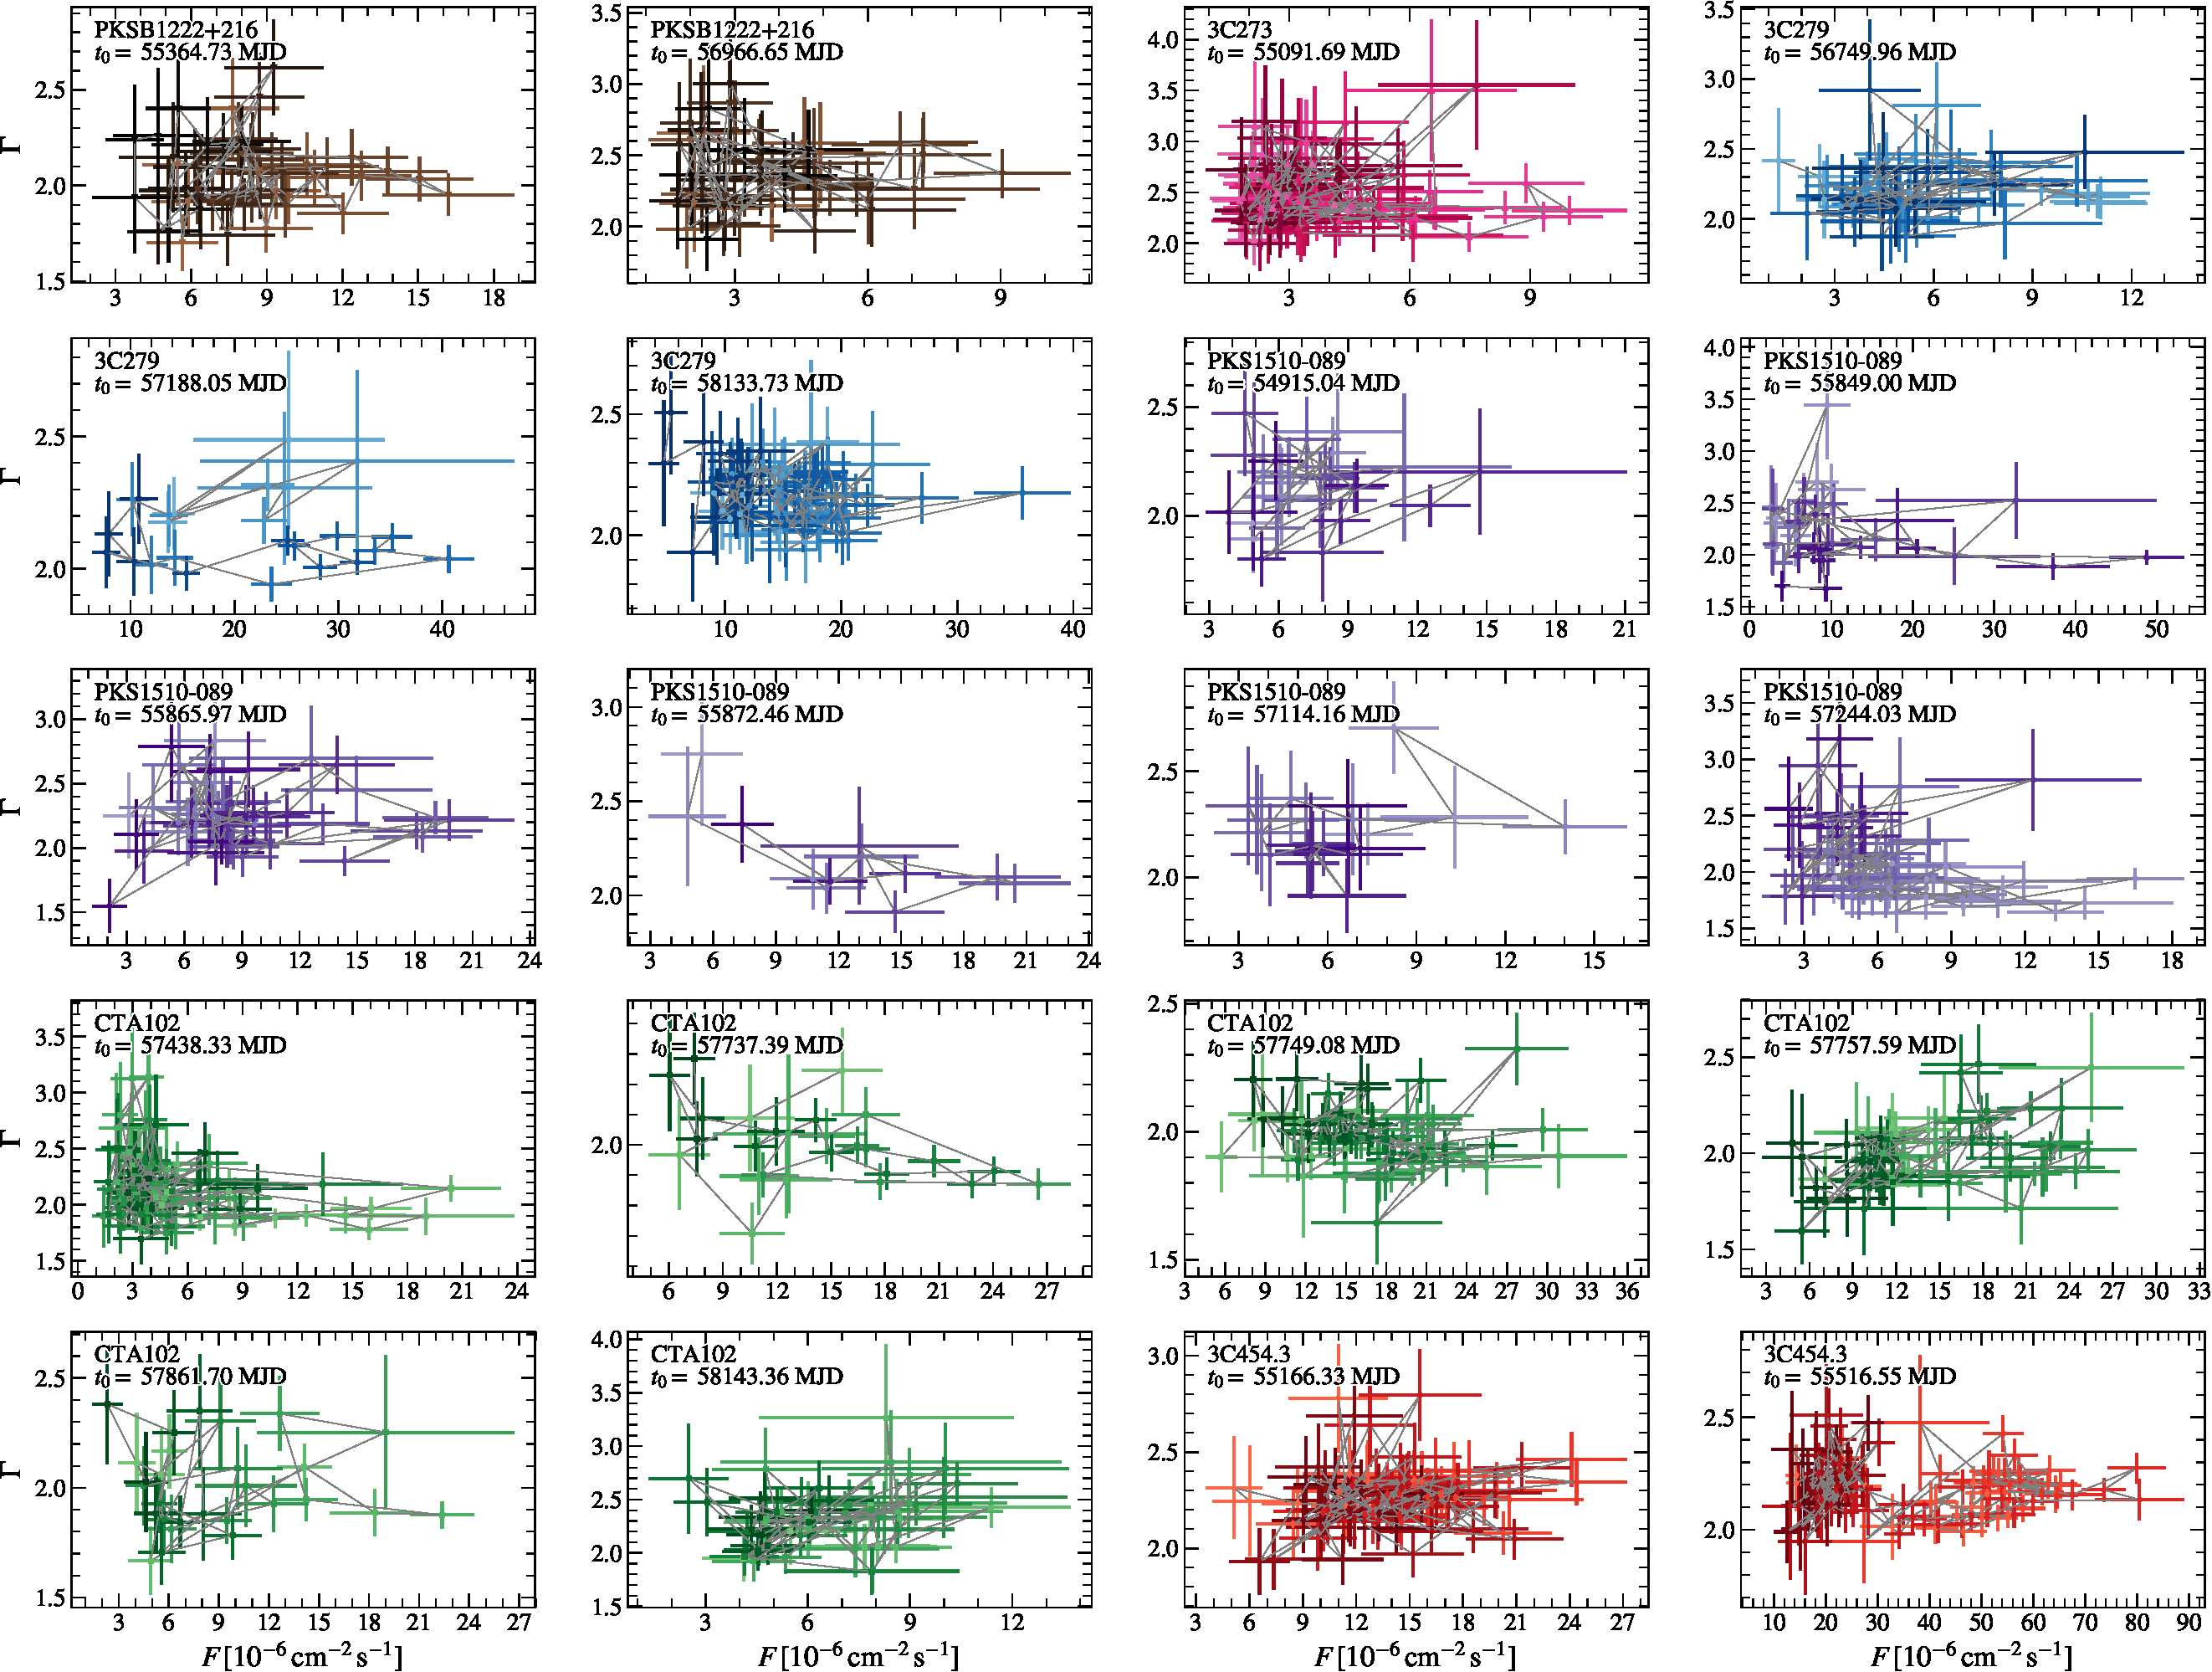
\includegraphics[width = .9 \linewidth]{figures/lc_specvar_flare_int.pdf}
    \caption{Spectral variations of the brightest flares on orbital time scales. Light colors refer to earlier times, dark colors to later times.}
    \label{fig:specvar}
\end{figure*}
\end{appendix}

\bibliography{mainbib}

%% This command is needed to show the entire author+affilation list when
%% the collaboration and author truncation commands are used.  It has to
%% go at the end of the manuscript.
%\allauthors

%% Include this line if you are using the \added, \replaced, \deleted
%% commands to see a summary list of all changes at the end of the article.
%\listofchanges


\end{document}

% End of file `sample62.tex'.
